\documentclass[justified,nobib]{tufte-book}

\setcounter{secnumdepth}{2}


\usepackage[backend=biber,style=authoryear]{biblatex}
\addbibresource{references.bib} 

\DeclareSourcemap{
  \maps[datatype=bibtex]{
    \map{
      \step[fieldset=urldate, null]
    }
  }
}


\usepackage[utf8]{inputenc}

\usepackage{amsthm}
\usepackage{amssymb}
\usepackage{amsmath}
\usepackage{mathrsfs}

%For typesetting a few things in the text
\usepackage{dialogue}
\usepackage{customdice}
\usepackage{booktabs}

\usepackage{graphicx}
\usepackage[]{hyperref}

% For game theory stuff
\usepackage{tikz-qtree}
\usepackage{sgame}

% I need this to make some crossed out symbols
\usepackage{cancel}

%Try etoolbox for conditional compliation if I want to go that route.

%For making the list of symbols
%\usepackage[intoc]{nomencl}
%\makenomenclature
%\renewcommand{\nomname}{List of Symbols}

% Instead of having a list of symbols, I'm putting them as margin notes instead:
\newcommand{\nomenclature}[2]{\marginnote{#1: #2}}



\hypersetup{
    bookmarksnumbered=true,     
    bookmarksopen=true,         
    bookmarksopenlevel=1,       
    colorlinks=false,            
    pdfstartview=Fit,           
    pdfpagemode=UseOutlines,  
    pdfpagelayout=TwoPageRight
}

\newtheorem{proposition}{Proposition}
\newtheorem{definition}{Definition}
\newtheorem{lemma}{Lemma}

\DeclareMathOperator*{\argmax}{arg\,max}

\newcommand{\breakslash}{\slash\hspace{0pt}}

\title{Theories of Rational Decision}
\author{Kevin Zollman}

\begin{document}

\maketitle

\newpage
\begin{fullwidth}
~\vfill
\thispagestyle{empty}
\setlength{\parindent}{0pt}
\setlength{\parskip}{\baselineskip}
Copyright \copyright\ \the\year\ Kevin Zollman

\par This version was created on \today

\par Licensed for non-commercial use, distribution, and modification with the CreativeCommons BY-NC-ND license version 4.0. Find more information here: \url{https://creativecommons.org/licenses/by-nc-nd/4.0/}


\end{fullwidth}

\tableofcontents

\chapter{Introduction}

``That's irrational!''

This is a phrase you have undoubtedly heard many times before. There's a good chance that you've uttered it or a close relative.  Perhaps many times.  

People are accused of being irrational in how they vote, in what they buy, in the job the take, in their choice of education, because they gamble, because they take too many risk or not enough, because of what they do or don't believe. Etc. Etc. Etc.

Even the most conservative among us recognizes that different people like different things.  While we might be tempted to equate ``rationality'' with ``what would I do,'' most of us know better than that.  I love pasta, but I don't think it's irrational for someone who is gluten intolerant to avoid eating it.

On the other hand, I don't think that most of us view any collection of decisions as rational. A person who drives those they love away from them is behaving irrationally. Millions of people seek out professional help in order to try and get their behavior to better match what they want from themselves.

The study of rational behavior is called ``decision theory.'' Decision theory is\dots no surprise\dots the study of how people make decisions.  That study is broken down into two parts.

First, is something called ``descriptive'' or ``empirical.'' We want to understand how people make choices, and we would like to have a generalized model of those decisions. We might want to predict, for example, what kind of peanut butter you might buy when you go to the store to buy peanut butter, or where you might choose to live, or even whether you will spend the rest of your life with your current significant other.  Such a model has wide applications from psychology, artificial intelligence, economics, sociology, and even epidemiology.

The other application is ``normative.''  However people actually behave, we might be interested to know how they {\it ought} to behave.  What does it mean for someone to make an irrational choice? What about a rational one? This application of decision theory attempts to build a theory that will distinguish rational from irrational choices.  Good choices from bad ones.

This second application has obvious philosophical implications, but it also has many others.  If we want our policies to be ``rational'' then we might want to require that our regulatory bodies use this theory.  If we want to design an AI to make rational decisions, we might want to use this theory. Etc.

You may have heard of {\it maximizing utility} (or even maximizing {\it expected} utility).  In many fields, like economics and computer science, this is treated as the only rational way to decide.  The reasons for this are complicated, and we will investigate them here. One way to understand these notes is as an exploration of why people are so enamored with this way of deciding, and what it actually means. If you have heard of these terms before, you may be surprised to learn what it does and does not mean.

In these notes, we will focus on the mathematical core of decision theory.  As we develop that core, we will have an eye to both applications.  Of course, we can't possibly cover all the theory, much less the applications of it. I hope that by the end of these notes you will have a basic understanding of the core theory.

I say ``core'' here because there really isn't a single thing that is decision theory. Rather there are many decision theories.  What I will be presenting to you is the received view: the thing people usually mean when they refer to decision theory.  I will note along the way various departures that one might take, but we won't follow them up.  Those departures might go in very different directions depending on whether our aim is normative or descriptive, and that's okay.

\marginnote{Much of the mathematical content of these notes is built off of the brilliant textbooks: \fullcite{kreps1988} and \fullcite{fishburn1979}} The basics of decision theory is mathematical.  We will use the tools of mathematics to develop the theory.  Our hope is that the precision of mathematics can help us to avoid equivocation and provide a clear articulation of the consequences of the theory.  Of course, mathematization runs the risk of hiding important distinctions behind the choice of representation.  I will try to point out when a decision theorist might be accused of doing this.  This isn't meant to be a criticism of mathematization, but a call for---perhaps---a different representation.

In terms of what kind of mathematics we'll be using, it is not difficult.  We'll be using some basic ideas from set theory and algebra.  Decision and game theory can be expanded to more complex setting where one might use calculus, analysis, and topology, but for these notes we won't go there.  I will also mostly avoid issues that arise only in infinitely large settings.  Those can be interesting, but I'd rather not be distracted by them in these notes for the purpose of introduction.


\chapter{Decisions under certainty}
\label{c:certainty}

Although much of decision theory is focused on decisions where there is some degree of uncertainty, we will start with a far simpler setting: deciding between known options.  Here our decision maker---we'll call her Mandy---faces a simple choice: she must pick which, from a set of possible things, she would want to have or bring about. Suppose Mandy is a judge in a painting contest.  She sees the paintings that have been entered in the contest, she has no uncertainty about what painting she is looking at. She simply must select which she would like to choose as the winner.

In one respect these are ``simple'' decisions because all Mandy must decide is what thing she prefers; she does not have to try and evaluate uncertainty.  When the judge selects a winner, she knows what will happen and what the winning painting will look like. On the other hand, the decision may not be simple because the options might be quite hard to compare. Our judge may have difficultly deciding which painting she prefers even though there is no uncertainty in the technical sense of that word.

There is some debate about how often we really find ourselves in this circumstance.  If Mandy goes to a restaurant, even one she knows well, and she orders a burrito, is this a situation of decision under certainty?  In one sense, yes.  She will almost certainly get a burrito.  But it is possible that the burrito might be better or worse than normal or it might contain an unexpected ingredient. More radically, perhaps Mandy doesn't know how much she will enjoy a burrito today. She's uncertain about her own reaction.

Whether or not these decisions are common, we will start here because they are simpler and they allow us to lay the ground work for decisions with uncertainty later.

\section{Preference and indifference}

We will start with a simple question: what does it mean to prefer one thing over another?  This might seem so simple as to not need inquiry, but we will inquire nonetheless.

Let us start by supposing that Mandy has a set of potential objects under consideration: an apple, some cherries, and a banana.  We will ask Mandy what she prefers from this set.  In particular, we will ask her to chose from among each possible pair which option she prefers.  

``Prefers'' is already a tricky concept.  It can mean several different things in different contexts.  Importantly it might mean different things in the normative and descriptive context, and its relationship to someone's behavior might be somewhat tenuous.  We won't get into this issue now, instead we will take ``prefers'' as a kind of primitive of the theory.

Prefers, for the moment at least, will be defined on pairs of objects.  Mandy prefers one object $x$ to another object $y$.  This allows us to represent preferences with a mathematical relation, denoted: $x \succ y$. There may be times that Mandy cannot answer, because she does not have a preference for one over the other.  In such a case, we will define another relation which we call ``indifference'' and this will be symbolized by $x \sim y$.

\nomenclature{$x,y,z$}{Arbitrary prizes. These might be objects of choice directly, or the result of chosing a gamble and being awarded this}
\nomenclature{$\succ$}{Strict preference. $x \succ y$ is read as ``One strictly prefers $x$ to $y$.'' Sometimes written with a subscript to denote a particular person's preference or a preference according to a certain standard. $\succ_i$ indicates preference according to $i$.}
\nomenclature{$\sim$}{Indifference. $x \sim y$ is read as ``One is indifferent between $x$ and $y$.'' Sometimes written with a subscript to denote a particular person's preference or a preference according to a certain standard. $\sim_i$ indicates indifference according to $i$. }
\nomenclature{$X$}{The grand set of all possible prizes.}

We will make a series of assumptions about the mathematical structure of these two relations.   To do so, we will assume we have some grand list of (potential) options over which the relations are defined.  Let that set be denoted $X$. The assumptions are divided into three groups.
\begin{itemize}
    \item Constraints on $\succ$
    \begin{itemize}
        \item $\succ$ is irreflexive: it is never the case that $x \succ x$ (or we might write this: for all $x \in X$, $x \nsucc x$)

\nomenclature{$\in$}{Set theoretic membership. $x \in X$ is read as ``$x$ is in the set $X$.''}
        
        \item $\succ$ is asymmetric: if $x \succ y$ then $y \nsucc x$
        \item $\succ$ is transitive: if $x \succ y$ and $y \succ z$, then $x \succ z$
    \end{itemize}
    \item Constraints on $\sim$
    \begin{itemize}
        \item $\sim$ is reflexive: for all $x \in X$, $x \sim x$
        \item $\sim$ is symmetric: if $x \sim y$ then $y \sim x$
        \item $\sim$ is transitive
    \end{itemize}
    \item Joint constraints
    \begin{itemize}
        \item Strictness: if $x \succ y$ then $x \nsim y$
        \item Joint completeness: for all $x$ and $y \in X$: either $x \succ y$, $y \succ x$, or $x \sim y$
        \item Joint transitivity: if $x \succ y$ and $y \sim z$, then $x \succ z$
    \end{itemize}
\end{itemize}

\marginnote{As an exercise, can you figure out which one of these nine conditions is entailed by the other eight?} In order to highlight important properties, I've actually listed more properties than is necessary.  One of these nine properties is entailed by the other eight.

We could have done everything more simply and cleanly by starting with a slightly less intuitive relation.  Consider $\succsim$, which means something like ``not worse than.''  If $x \succsim y$, then we would say that $x$ is not worse than $y$.  If we start with $\succsim$ we can define $\succ$ and $\sim$ in terms of it
\begin{definition}
\label{d:succ}
$x \succ y$ if and only if $x \succsim y$ and {\bf not} $y \succsim x$
\end{definition}
\begin{definition}
\label{d:sim}
$x \sim y$ if and only if $x \succsim y$ and $y \succsim x$
\end{definition}

\nomenclature{$\succsim$}{Weakly preferred to.  $x \succsim y$ is read as ``One weakly prefers $x$ to $y$'' or ``One either pefers $x$ to $y$ or is indifferent between them.'' Sometimes written with a subscript to denote a particular person's preference or a preference according to a certain standard. $\succsim_i$ indicates preference according to $i$.}

With this definition we can now capture the nine constraints above with a far simpler representation.  We can just say that $\succsim$ is transitive and complete.  

We defined transitivity above, so I won't repeat it here.  Completeness is also quite simple, it requires that for every $x, y \in X$ at least one of these hold $x \succsim y$ or $y \succsim x$.  Of course, in some cases both might hold.

Because of its mathematical simplicity, most decision theorist define preference in this simpler way using $\succsim$ and then define the strict relations $\succ$ and $\sim$ in terms of it.

\marginnote{As an exercise you might try to prove that if $\succsim$ is complete and transitive and if we define $\succ$ and $\sim$ in this way, that all of the nine conditions hold.  Do you always need both completeness \emph{and} transitivity?} If we follow this mathematically more elegant way of defining the preference relation, all of those nine properties listed above become theorems that one can prove using only the transitivity and completeness of $\succsim$.  Let me show you how you can prove the transitivity of $\succ$ if it is defined according to definition~\ref{d:succ}.

\begin{proposition}
If the relation $\succsim$ defined over $X$ is transitive and $\succ$ is defined according to definition~\ref{d:succ}, then $\succ$ is transitive
\end{proposition}

\begin{proof}
Suppose that $x, y, z \in X$ and that $x \succ y$ and $y \succ z$.  Since $x \succ y$ then by the definition of $\succ$, $x \succsim y$.  Similarly since $y \succ z$, then $y \succsim z$.  Since $\succsim$ is transitive by assumption, this means that $x \succsim z$. 

Now we must show that it is not the case that $z \succsim x$.  Suppose that it was the case that $z \succsim x$. We have already shown that $x \succsim y$, so by transitivity, this would mean that $z \succsim y$.  However, we assumed that $y \succ z$, which by definition requires that it not be the case that $z \succsim y$. This contradicts our assumption.

Since we have shown that $x \succsim z$ and it is not the case that $z \succsim x$, by definition this entails that $x \succ z$
\end{proof}

Since the two ways we define it are mathematically equivalent, why not just use the simpler one?  Part of the reason I include the more complex definition, is that it allows us to pinpoint  what constraints might exhibit problems when we consider this from both the normative and descriptive perspective.  It is to this that we now turn.

\section{Problems and paradoxes}

\subsection{Incommensurability and completeness}

Built into our definitions is the assumption that any two objects can be compared, the is the {\it joint completeness} constraint for $\succ$ and $\sim$ or alternatively the {\it completeness} constraint for $\succsim$.  In many everyday contexts, this seems quite natural, but there are also situations where this might be quite difficult.  

The philosopher Ruth Chang, for example, asks the question: was Mozart a better composer than Michelangelo was a painter?\marginnote{For several different philosophers take on this problem see \fullcite{chang1998}}  This strikes many of us as a strange question, how can we compare across these two different media?  Someone who loves both classical music and Renaissance painting might be incapable of saying whether they prefer the music of Mozart or the paintings of Michelangelo.  

In such cases we might opt to say that two things are incommensurable, they are simply not comparable.  It would be wrong to say that one is better than the other, {\it but also wrong to say they are equivalent.}  It is that last clause that creates the problem for the decision theorist.  Because, under our assumptions, if you don't say that Mozart is better than Michelangelo or the reverse we are forced to say one is indifferent.

To see why this might frustrate some people, consider Sophie's choice from the famous novel.\marginnote{\fullcite{styron1979}}  Sophie must choose which of her children will die.  She loves them equally, so she cannot decide which she prefers.  Under our axioms, if she cannot choose one over the other, then we would say she's indifferent.  

What's wrong with that?  Suppose just before she was forced to make her choice, someone came along and said ``I know this is a difficult decision for you, Sophie.  I want to make things easier.  Here, I will put \$10 in your daughter's pocket.'' Does this make Sophie's decision easier?

Of course it doesn't.  The devastating issue for Sophie is not that she's indifferent between her two children, where any simple tie-breaker will resolve her indifference.  Rather, she cannot make a comparison.  When it comes to her children, Sophie does not obey our axiom of {\it joint completeness.}

As is the case with all of our objections, we can ask two different questions about this example.  The first question: is it descriptively plausible?  That is, do we think that people might often find themselves in a situation where they cannot form a preference?

This question is actually somewhat difficult to answer unless we put some structure on what we mean by ``preference.''  At first blush it seems quite right that we often don't have preferences.  Which is my favorite town in North Dakota? I have no preference, because I have never been to any towns in North Dakota. With all due apologies to people from North Dakota, I have also given very little thought to the towns there. I know nothing about them.

At this level of description, completeness is obviously wrong: I simply don't have a preference.  It would also seem strange to say that I'm indifferent.  I just haven't ever thought about it.

Often in discussing this theory, ``preference'' is given a more counterfactual interpretation.  It's true that I, at the moment I'm writing this, don't have a preference between towns in North Dakota.  If I won a contest that involved an all-expense-paid trip to a North Dakota town of my choice, I would investigate and form a preference.  

Many economists define ``preference'' in this theory in a purely behavioral way.\marginnote{To learn more about this way of thinking and objections to it, see \fullcite{thoma2021}}  For these economists, to prefer something is simply to choose it (or to be disposed to chose it if given the chance).  If preference is defined in this way, incommensurability has less force.  At the end of the day most of would choose one thing or another if forced to do so.  While this behavioral way of defining preference makes completeness true by almost by definition, it puts more pressure on the other axioms.

Another dimension to the descriptive question is to ask exactly what we mean by descriptively correct.  Humans are incredibly varied and complicated. No one doubts that somewhere in the history of our species someone has violated these axioms.  I know of no theorists who thinks they are like physical laws that constrain everyone, everywhere.  The debate about their descriptive accuracy is more of one of degree: how often and under what conditions do people behave in accordance with these axioms?  Some people think most of the time we do, that violations are rare.  Others think that violations might be more common or happen in critical enough situations that the axioms are not as accurate as we might need them to be.

The second version of the question one might ask about this axiomatiziation: is it normatively correct? Of course it might be that our real preferences sometimes violate these axioms, but that when they do we regard this as a kind of personal failure.  You might point out the failure to me, and I would say ``Oh! That was stupid of me'' and attempt to correct it.  However, there may be cases where you point out the violation, and I say ``Well, so much the worse for axioms. I think my behavior is correct.''

On the normative side we must address the same thorny interpretative question that we needed to address on the descriptive side.  What do we mean by a preference?  Is this a constraint on some kind of psychological state, on a disposition to have a psychological state, or a disposition to choose when forced.  And just as for the descriptive interpretation of the axioms, one might have a different normative judgment depending on how they are interpreted.

In order to ask this question, let's look at three problems that have been raised for both the normative and descriptive interpretation of these axioms.  (We will introduce several more in section~\ref{s:choice-functions}.)

\subsection{Preference change}

Of course, you could not represent one's entire life with a single preference relation.  When I was a young child, I would certainly have preferred candy for dinner to almost anything else.  As an adult, I might still occasionally be tempted, but I (almost) never choose it.  Does that mean that the theory is already obviously wrong?

Most people who use the theory would say ``no.''  The theory is about preference {\it at a time}. That is: Mandy's preferences at this exact instant obey the axioms, but not that Mandy's preferences can't change.  So long as at each time, Mandy's preferences obey the axioms, then she's fine, even if those preference are quite different from one another.

This simplifies the theory, but it also introduces some difficulties.  The first is with empirical test.  I cannot at this very moment offer Mandy more than one choice. I can offer Mandy one choice and then, perhaps seconds or minutes later, offer her another.  If it appears that Mandy violates the axioms, it remains a possibility that her preferences have changed in a way that makes it look like a violation (when it really isn't).

So, in reality, we must assume that preference are somewhat stable over time.  If they change rapidly, it might be indistinguishable from a violation of the axioms.  What's more, it might make any theory built on those axioms somewhat useless, since the theories will use a stable set of preferences.

One must also keep this in mind when thinking about {\it what} the theory is defined over.  That is, some preferences might change very quickly as someone learns new information.  If Mandy is offered the option to purchase a delicious looking burrito for a bargain price, she might be glad to take it.  If she discovers that the burrito is, in fact, two weeks old, she might quite rapidly change her preferences.

Often, people want to focus the theory on basic or fundamental preferences which change relatively slowly over time.  Mandy enjoys time with her friends.  And while her particular group of friends may be different over the years, her preference for spending time with friends may stay relatively constant.

\subsection{Paradox of preference}

\marginnote{This example is a modified version of one in \fullcite{anand1993}} Sometimes the particular paired choice that Mandy faces cues her to think about the choice in different ways. Suppose that Mandy goes to a friends house for tea and cookies.  Mandy loves cookies. We might imagine the following three situations:\marginnote{Please note, Mandy isn't being offered these in turn. Rather we are imagining how she might behave if given one of these choices at the outset.}
\begin{enumerate}
    \item Mandy is offered the choice between a large oatmeal cookie and a large chocolate chip cookie. Mandy has a slight preference for oatmeal cookies, so she chooses that one.
    \item Mandy is offered the choice between a large chocolate chip cookie and a small oatmeal cookie. While she slightly prefers oatmeal, the size difference matters more. She chooses the large chocolate chip cookie. She's worried that choosing the larger cookie will seem greedy to her friends, but she knows that she can just lie and say ``I prefer chocolate chip.''
    \item Mandy is offered the choice between a large oatmeal cookie and a small oatmeal cookie. While she wants the bigger one, she's worried it will seem greedy to take the larger of the two. No lie is available here, so she opts for the small cookie.
\end{enumerate}

Mandy's choice behavior violates transitivity. That occurs because different choices induce different ways of thinking about the choice. She wants bigger cookies when she can get them without seeming greedy. 

For Mandy we might ask two different questions.  First, does this seem like a plausible empirical setting, one where we might expect people to habitually make these choices? 

We might also ask whether we regard Mandy's choices as reasonable. Take a moment to think about your reaction to this situation.  If you pointed this out to Mandy, do you think she should recognize what happened as a mistake and revise her choices?  Or should she dig in her heals and say she was right to have those preferences?

\subsection{Quinn's paradox}

Suppose that someone is deciding whether to engage in a fun activity that carries with it a small risk.  For example, suppose that there is an ongoing pandemic, and Mandy must decide whether to have a small group of friends over this evening for drinks.  Mandy has many friends, and she must decide how many of her friends to invite.  As a somewhat obnoxiously pedantic person, Mandy starts by forming a list from the person she most want to invite (at position \#1) to the person she least wants to invite (at position \#$n$). 

Now she must form a preference ranking over the options ``invite the first $x$ people on the list'' where $x \in {0, 1, \dots n}$.  We will denote each option by $O_x$, so $O_1$ means invite the top person, $O_2$ means invite the top two, and $O_n$ means invite everyone.  $O_0$ means ``don't invite anyone.''

Our host reasons as follows, ``the disease is not common in my city and the health minister said that we can have small gatherings.  So, it is okay to have one friend over.'' Thus, $O_1 \succ O_0 $.

Also, she thinks ``inviting one additional person will only increase the probability of catching the disease slightly. I really wouldn't want to hurt my friend's feelings. I think the kindness of inviting one additional person is worth the very small increase in risk from the disease.''  As a result they form the preference $O_{x + 1} \succ O_x$ for all $x \geq 1$.\marginnote{This is not exactly how Quinn put his paradox, I have modified it to be about a different topic. To see the original version, check out \fullcite{quinn1990}}

\nomenclature{$>$}{Numerically greater than. Not the same as $\succ$}
\nomenclature{$\geq$}{Numerically greater than or equal to. Not the same as $\succsim$}

However, the health minister is very clear that there can be no large gatherings.  Our host doesn't quite know what large is, but she is quite certain that $n$ is large. She wants to obey the health minister, so $O_0 \succ O_n$. This set of preferences violates our axioms.

This violation is related to something known as a just-noticeable-difference in psychology.  If I play you a tone that is 60 dB loud, you cannot tell that it is louder than another tone that is 60.5 dB loud.  That is less than your just-noticeable difference for sounds.  Similarly you could not tell the difference between 60.5 dB and 61 dB.  Many people can, however, tell the difference between 60 and 61 dB.

Like with all questions we can approaches this from both a descriptive and normative perspective.  From a descriptive perspective, just noticeable differences are a well confirmed phenomenon for all modes of perception. Do such problems ``scale up'' in the way I described?  Obviously Mandy can tell the difference between having three and four friends over, but she treats them as ``the same.''  Insofar as we categorize things this way, we might expect to find violations of transitivity.  

\marginnote{For arguments against our axioms as normative requirements, see \fullcite{temkin1996}}\marginnote{For a defense of our axioms, see \fullcite{binmore2003}} Beyond the descriptive question, it's less clear if this is normatively correct.  Some philosophers have argued just that, although many others are skeptical.

\section{Beyond pairwise comparisons}
\label{s:choice-functions}

So far we have focused on making decisions as pairwise comparisons.  Is $x$ better, worse, or the same as $y$?  However, in many real world settings we are giving the choice between many different options all at once.  When you go to a restaurant, you usually see a menu with many options, not just two.

A common initial reaction is to say, ``can't we just think about big choices as many pairwise choices?'' First, Mandy compares option \#1 on the menu to option \#2, and chooses her favorite.  Then the winner of that contest is paired against option \#3, etc.  Eventually Mandy reaches the end of the menu and whoever survives is the winner. Indeed that's how many economists think about it.  

Of course, we don't {\it have} to think of it that way.  Forcing people to make decisions like this or assuming they do adds structure. It makes impossible patterns of choices called {\it menu dependence}, which we might want to at least entertain before dismissing them.  But to articulate what is menu dependence requires a slightly more general formalism.

\subsection{Choice functions}

To start we will suppose that there is a grand list of options $X$.  One might not always be confronted by all these options, instead this represents all the potential options Mandy might face.  Think of it like the list of all potential dishes that she might find on any menu of any restaurant.

A given choice will present Mandy with a subset of $X$, $M \subset X$ that we will call a ``menu.''   The power set of $X$, denoted by $\mathscr{P}(X)$ is the set of all subsets of $X$, or for our purposes, the set of all potential menus.

\nomenclature{$M$}{A menu. A set of choices that an agent might face.}
\nomenclature{$\subset$}{Strict subset. $M \subset X$ is to be read as ``$M$ is a strict subset of $X$.'' This means that every member of $M$ is a member of $X$, but there is at least one member of $X$ that is not a member of $M$.}
\nomenclature{$\subseteq$}{Weak subset. $M \subseteq X$ is to be read as ``$M$ is a subset of $X$.'' This means that every member of $M$ is a member of $X$.}
\nomenclature{$\mathscr{P}(X)$}{The powerset of the set $X$, that is a set containing all subsets of $X$.}

Mandy's job is to choose an option or set of options from that menu which she regards as acceptable.  To represent all of Mandy's choices in all potential situations, we will use a function $c$.  To start, we will impose very weak constraints on the function.  We make three assumptions about choice functions:
\begin{enumerate}
    \item $c: \mathscr{P}(X) \to \mathscr{P}(X)$
    \item $c(M) \subseteq M$
    \item $c(M) \ne \emptyset$
\end{enumerate}
The first condition, just says that $c$ is a function from menus to other menus.  The second means that $c(M)$ contains only options that are in $M$ (you can't choose something that is not on the menu).  And the last says that $c$ must choose {\it something} that's on the menu.

\nomenclature{$c(\cdot)$}{A choice function. This takes as input a menu of options and outputs those options that the agent would choose from that set (potentially more than one).}
\nomenclature{$\to$}{Defining a function. $c: X \to Y$ means a function $c$ which takes as input a member of the set $X$ and produces as output a single member of the set $Y$.}

Sometimes people are tempted to allow $c(M) = \emptyset$ with the idea that Mandy might opt not to choose anything. If one isn't worried about being rude, one can go to a restaurant and order nothing at all.  This makes an important point about how $M$ is interpreted. $M$ is supposed to include {\it everything} Mandy could do.  If ordering nothing is an option, then $M$ must include an option to ``order nothing.''  That means that $c(M) \ne \emptyset$ is a more reasonable constraint, since there is a ``order nothing'' option in $M$ if that is a choice Mandy might make.  

\nomenclature{$\emptyset$}{The empty set. That is, the set that contains no members.}

$c(M)$ represents how Mandy would choose if given the menu $M$.  The one strange feature of how we've defined it is that $c(M)$ is a set, not a single option.  At a restaurant you usually order one thing, or if you order more than one you intend to get more than one dish.  That is not how we are reinterpreting $c(M)$, though.  $c(M)$ is those things that Mandy would not pay an arbitrarily small amount to remove.  Whatever is left are those that are ``tied for best'' for her.  To put it another way, she is indifferent between all options in $c(M)$.

\subsection{Menu dependence}

So far $c$ as a function is pretty unconstrained. It does require that when confronted with the same menu, Mandy gives same answer.  This is equivalent to assuming that Mandy's preferences stay stable over time.  Beyond that, there is little to force any kind of consistency across menus.  

To illustrate how this might be a problem I always give a short little dialog.  Imagine that Mandy is in a restaurant listening to the specials from the waiter:

\begin{dialogue}
\speak{Waiter} Today we have two specials: mapo tofu and fish flavored chicken
\speak{Mandy} If those are my options, I definitely prefer the fish flavored chicken.  Please bring me that!
\speak{Waiter} Oh! I'm sorry, I just forgot. The chef added a third special at the last minute.  We also have strange flavor beef.  
\speak{Mandy}  That changes everything!  Thank you for telling me. In that case, I would definitely prefer the mapo tofu.
\end{dialogue}

Most people reading this story think that something strange has gone on.  If Mandy wanted to order the fish flavored chicken when she thought the menu was $\{$chicken, tofu$\}$ then she indicated that she wanted fish flavored chicken more than mapo tofu. If the menu then expands, she might change her mind to order the new dish instead.  But she shouldn't go back and change her mind regarding the two dishes that were already available to her.

\nomenclature{$\{\}$}{Used to denote a set of objects, $\{x,y,z\}$ is the set made up of elements $x, y,$ and $z$.}

Notice also that Mandy's choices make it impossible for us to represent her with a preference relation $\succsim$.  Does she prefer mapo tofu over fish flavored chicken or vice versa (or is she indifferent)?  None of those options can account for her choices in our little dialog.

The more general name for what Mandy did was ``menu dependence.''  Whether she preferred the tofu or the chicken depended on what menu was presented to her.  When the menu was $\{$chicken, tofu$\}$, she preferred the chicken to the tofu. When the menu was $\{$beef, chicken, tofu$\}$ she preferred the tofu to the chicken.

\subsection{Sen's $\alpha$ and $\beta$}

The story of Mandy in the restaurant shows that the choice functions and preferences are not, at base, the same formalism.  Although I haven't proven it formally, choice functions are strictly more general: someone who makes only pairwise choices can be represented with a choice function, but there are some choice functions (like Mandy's) that cannot be captured as a series of consistent pairwise choices.

\nomenclature{$\alpha$}{Sen's principle $\alpha$. A principle that constrains choice functions}
\nomenclature{$\beta$}{Sen's principle $\beta$. A principle that constrains choice functions}

One might like to know what additional constraints we might add which would allow us to ``read off'' someone's preferences from their choice function and vice versa.  That is, what additional assumptions would we need to impose to make these two equivalent?

There are a variety of different ways to axiomatize it, but the most clear is Amartya Sen's $\alpha$ and $\beta$ constraints.\marginnote{Sen himself discussed $\alpha$ and $\beta$ extensively in several papers collected in \fullcite{sen2004}}

\begin{definition}
({\bf Sen's $\alpha$}): Suppose that $x \in B$, $B \subseteq A$, and $x \in c(A)$, then $x \in c(B)$
\end{definition}

Mandy violated Sen's $\alpha$.  To see why, we can interpret the parts.  $x$ is the tofu.  $A$ is the larger menu $\{$beef, chicken, tofu$\}$.  $B$ is the smaller menu $\{$chicken, tofu$\}$.  The first conditions are satisfied.  $x \in B$, $B \subseteq A$, and $x \in c(A)$ since she ordered the tofu from the larger menu.  However, Mandy violated Sen's $\alpha$ because $x \notin c(B)$ since she ordered the chicken.

Although Sen's $\alpha$ has gotten rid of our example of Mandy above, it is not sufficient to ensure that someone behaves as if they have a preference relation.  We haven't yet made sure that people don't do strange things with ties.  

Suppose for example that Mandy's friend, Sean was with her and also heard the same menu.  Being a somewhat obnoxious restaurant goer, after hearing the first menu, Sean declared ``I don't care, bring me either one.''  However, upon learning of the presence of the beef dish, he changed his mind.  ``In that case, I'm not indifferent.  Bring me the chicken and definitely not the tofu.''  This is also inconsistent with thinking of Sean as having a preference relation. We need to exclude it as well.

\begin{definition}
({\bf Sen's $\beta$}): Suppose that $x, y \in c(B)$ and $B \subseteq A$, if $y \in c(A)$, then $x \in c(A)$
\end{definition}

These two conditions jointly entail that someone's choices will be consistent with them having a pairwise preference relation.  At the moment, that's stated a bit informally.  To make it more precise we need to say what it means to be ``consistent with'' a preference relation.

First, suppose that we have a grand menu $X$ and a choice function $c$ defined over it.  We will start by defining a relation (what will eventually be our preference relation) by looking at all the choices from menus with only two options on them. 

More precisely, let $R_c$ be defined as follows: for every $x, y \in X$, $x R_c y$ iff $x \in c(\{x,y\})$.  $x R_c y$ represents the relation ``$x$ would be among those chosen in a pairwise choice between $x$ and $y$.''

\nomenclature{$R$}{An arbitrary relation. $x R y$ is to be read ``$x$ stands in relation $R$ to $y$. Sometimes written as $R_c$ for a relation defined in terms of a function $c$.}


We should stop here for a moment and ask about the properties of $R_c$.  First off $R_c$ must be complete.  (Can you see why?) However, without making some assumptions about $c$ beyond it being a choice function, we cannot guarantee that $R_c$ is transitive. There is nothing in the definition of the choice function that prevents $R_c$ from having ``cycles'' where $x R_c y$, $y R_c z$, and $z R_c x$.

Sen's $\alpha$ and $\beta$ are sufficient to prevent this.\marginnote{As an exercise see if you can prove this.}
\begin{proposition}
If $c$ obeys Sen's $\alpha$ and $\beta$ then $R_c$ (as defined above) is transitive.
\end{proposition}

Remember the question we started with: does Sen's $\alpha$ and $\beta$ guarantee that our agent's preferences behave {\it as if} they have a pairwise preference relation?  At this point we are part way there.  We have shown that every choice from a menu {\it that only contains two options} is consistent with a preference relation. But what about if there is a menu with more than two options?  We need to show consistency there too.

To do this, we will complete the circle and use $R_c$ to define a choice function.  Define the function $d: \mathscr{P}(X) \to \mathscr{P}(X)$ in the following way:  For every $M \in \mathscr{P}(X)$, and $x \in M$, $x \in d(M)$ iff there is no $y \in M$ such that $y R_c x$ and not $x R_c y$.  Note: if $R_c$ is transitive, then we are guaranteed that $d$ satisfies the criteria of a choice function (do you see why?). 

\nomenclature{$d$}{An arbitrary function.}

What we've done is create the new choice function $d$ which is exactly what someone would chose if they started with the preference relation $R_c$ and then chose based on pairwise comparisons.

So now, we want to show that $d$ and $c$ are the same.  This shows that {\it all} the choices in $c$ are equivalent to someone who had preference relation $R_c$ and chose according to it.  Graphically, this whole process is depicted in figure~\ref{f:sensalpha}.

\begin{marginfigure}
\centering
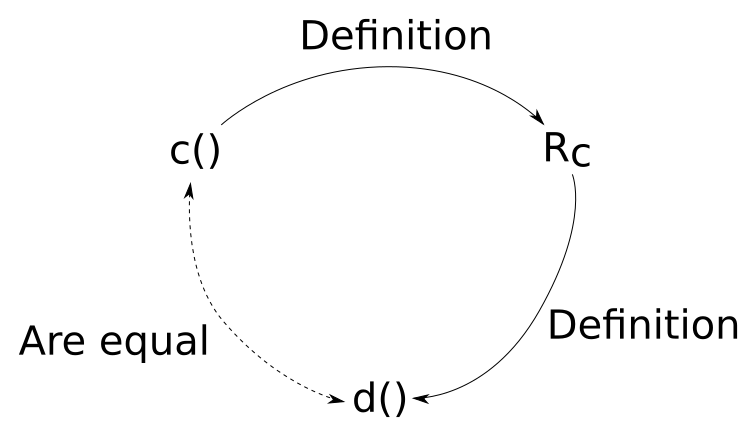
\includegraphics[width=\textwidth]{ChoiceFunctionDiagram.png}
\caption{A diagram of the construction process for proposition~\ref{p:sensalpha}.}
\label{f:sensalpha}
\end{marginfigure}

\begin{proposition}
\label{p:sensalpha}
If $c(\cdot)$ obeys Sen's $\alpha$ and $\beta$ then $c(\cdot) = d(\cdot)$
\end{proposition}
\begin{proof}
Suppose $M \in \mathscr{P}(X)$.  We need to prove two directions.  First that if $x \in c(M)$ then $x \in d(M)$ (we will call this ``$\Rightarrow$''). And, second, that if $x \in d(M)$ then $x \in c(M)$ (we will call this ``$\Leftarrow$'').
    
$\Rightarrow$: Suppose $x \in c(M)$ and suppose a $y \ne x$, $y \in M$ (if there is no $y$, this direction follows immediately). By Sen's $\alpha$, $x \in c(\{x, y\})$. So, therefore $x R_c y$. Since $y$ was arbitrary, we know that for all $y \in M$, $x R_c y$. This means that $x \in d(M)$

   
$\Leftarrow$: Suppose that $x \in d(M)$. Let $y \ne x$ and $y \in c(M)$. (If there is no such $y$ this direction follows immediately.) Since $x \in d(M)$ then we know that $x R_c y$ and therefore $x \in c(\{x,y\})$. Since $y \in c(M)$, $\{x,y\} \subseteq M$. By Sen's $\alpha$ $y \in c(\{x,y\})$. By Sen's $\beta$, $x \in c(M)$.
\end{proof}

Phew.  That was a lot of definitions, but at the end we've articulated something very important.  What does it mean to behave {\it as if} you are choosing according to a preference relation?  It means that you always obey Sen's $\alpha$ and $\beta$.

That allows us to approach a question we asked a while ago from a different angle.  The original questions were (a) is choosing {\it as if} you have a preference relation a normative requirement and (b) is it descriptive accurate?  Now we can ask that same question but in terms of Sen's $\alpha$ and $\beta$.  Is it normatively reasonable to require someone to obey $\alpha$ and $\beta$?  Is it descriptively accurate?

We will look at a few issues.

\subsection{Learning from the menu}

Sen himself didn't actually think his two conditions were either normative or descriptively accurate. He gave a series of examples that might present a problem, although the degree to which it does is controversial.

For the first counter example let's return to the restaurant. Again suppose that we have a restaurant goer Mandy who has wandered into a random restaurant without really looking into it at all.  She is listening to the daily specials.  At first, she hears two options: escargot and Hawaiian pizza.  The waiter is called away for a second and Mandy thinks, ``I like escargot, but I'm not sure that I want it from a place that also would make Hawaiian pizza. While I don't really want pizza, I think that's a safer bet.''

When the waiter returns, he provides several more options, all of which are traditional, high end French specialities.  Now, Mandy reconsiders. This must be a fancy French restaurant that is trying out a take on Hawaiian pizza. They probably do make good escargot, so she decides to order that.

This is a violation of Sen's $\alpha$ because escargot is chosen from the large menu, but is not chosen from the smaller menu containing only escargot and Hawaiian pizza. Not only does it seem plausible that someone might do this, but it also seems quite reasonable which suggests that $\alpha$ is neither descriptively accurate nor normatively correct.

Some people don't think this counts as a genuine objection, however. They point out that Mandy is learning something from the menu itself.  So, she's not really choosing (from her perspective) the same objects.  When she only knows about two dishes she thinks she's choosing between bad escargot and mediocre Hawaiian pizza.  In the larger menu she's choosing between good escargot and good pizza.  If we redescribe the situation where the escargot on the first menu is a different option than the escargot on the second menu, there is no violation of $\alpha$.

This general strategy is quite common when dealing with potential counterexamples to various constraints on preferences.  At the extreme one might {\it always} redefine the options to be different options under each choice scenario.  Of course this is a way to respond, but it runs the risk of making $\alpha$ and $\beta$ toothless.  At the extreme, if every choice situation involves novel choices, there are no consistency requirements whatsoever. Everyone is always facing a completely new menu.

\subsection{The role of social norms}

\marginnote{Sen discusses this example in \fullcite{sen2004a}}Sen raises another series of examples about how social and moral norms might cause these kinds of violations.

Imagine Mandy is now at a wedding where two types of fruit (mangoes and apples) are being served.  Mandy strongly prefers mangoes to apples, but Mandy also recognizes that there is a strong prohibition against taking the last of anything.  Mandy approaches the table with fruit and sees one mango and two apples.  We can imagine labeling these objects for convenience, let's call them $m_1$, $a_1$, and $a_2$.  In this setting, Mandy would opt to take one of the apples, since there is only one mango present. Stating this a little more formally, $c(\{m_1, a_1, a_2\}) = \{a_1, a_2\}$.

Now suppose that the caterer comes and adds another mango (let's call it $m_2$).  With the additional mango, Mandy is no longer taking the last mango.  So now, she would take one of the two remaining mangoes.  Stated more formally $c(\{m_1, m_2, a_1, a_2\}) = \{m_1, m_2\}$.  This violates Sen's $\alpha$.

The critical point here is that features of menu, combined with a social norm against taking the last of anything, creates a kind of dependence on the menu.  

Of course, ``don't take the last mango'' is a social norm, but if that's the only time this comes up one might think it an oddity. Sen thinks such examples are more ubiquitous and might occur in the context of many moral constraints.  Space will prevent our discussion of this in full here, but you might think about whether any moral norms might lead to violations of Sen's $\alpha$ or $\beta$.

\subsection{The decoy effect}

Behavioral economics, the place where many of these axioms are tested on humans, has provided several purported examples of menu dependence in everyday people. Some are controversial. {\it The decoy effect} is perhaps the most clear example, and has apparently been used by marketers for decades (or centuries?).

For an illustration, consider the following experiment.  Suppose that Mandy is given the opportunity to purchase a six-pack of beer. She knows only the price and the quality as judged by participants in a blind taste test.  She is first given the choice between the two options in table~\ref{t:decoy-two}.  Suppose that Mandy deicdes that she would prefer the cheaper beer, so she chooses option $x$.

\begin{table}
    \begin{tabular}{ccc}
    \toprule
     Option & Price & Quality (0 = worst, 100 = best) \\
     \midrule
     $x$    & \$18  & 50 \\
     $y$    & \$26  & 70 \\
     \bottomrule
    \end{tabular}
    \medskip
    \label{t:decoy-two}
    \caption{A two-choice menu}
\end{table}

Now suppose that instead, she had been given a different menu in table~\ref{t:decoy-three}.  It still includes options $x$ and $y$, but it includes a third option, $z$.  $z$ is obviously inferior because it is the same quality as $y$ but more expensive.  When this option is now on the list, Mandy chooses $y$ instead.  Now, $y$ seems like a good deal.

\begin{table}
    \begin{tabular}{ccc}
    \toprule
     Option & Price & Quality (0 = worst, 100 = best) \\
     \midrule
     $x$    & \$18  & 50 \\
     $y$    & \$26  & 70 \\
     $z$    & \$30  & 70 \\
     \bottomrule
    \end{tabular}
    \medskip
    \label{t:decoy-three}
    \caption{A three-choice menu with a decoy}
\end{table}

\marginnote{For this experiment and similar ones see, \fullcite{Huber1982}}Experiments with these options or ones like them, suggest that people may violate Sen's $\alpha$. The addition of ``decoys'' can cause people to change their preferences on the items listed.

There is a large literature documenting this effect, attempting to determine where it occurs, and trying to explain why it occurs. It's possible that it is an example of ``learning from the menu'' like the example of the wedding above, but I think it's fair to say that this is not fully settled yet.

\subsection{Differing dimensions of value}

In the previous section, we talked about incommensurability of objects. Sophie cannot choose between her two children, one might argue, because she simply does not have a dimension on which to compare them.  Difficult choices are made difficult, often, by the opposite problem: we have far too many dimensions on which they differ. 
\marginnote{This example is a modified version of one first presented in \fullcite{Levi1990}}

Let's consider a simple decision problem: where to go for dinner.  Suppose Mandy is deciding between three restaurants.  Al's Armenian, Bea's Bahamanian, and Charlie's Chechnyan; $a$, $b$, and $c$ for short.  Mandy cares most about the taste of the food and the quality of service.  Suppose she has decided that on the taste of the food $a \succ_F c \succ_F b$, and on the quality of service $b \succ_S c \succ_S a$.  (I'm using the subscripts here because these aren't Mandy's all-things-considered preferences, just her preferences according to a pre-specified dimension.)

When she decides on a restaurant she first eliminates all the restaurants that aren't the best according to taste or quality of service.  If Mandy is left with only one restaurant, she goes there.  If she is left with more than one, however, then she will break the tie with a third criteria: the quality of the decor.  On decor, she ranks the restaurants $c \succ_D a \succ_D b$.

This decision procedure will result in a set of decisions that violate Sen's $\alpha$.  Can you see why?

\section{Transitivity, completeness, and utility}

Why are we so concerned with transitivity and completeness to begin with?  One might just be interested in them for their own sake; to put some constraints on what it means to be rational. But often scholars are interested for another reason, that you have probably surmised: our ability to represent people with math.

We've often motivated some of the constraints on $\succsim$ by appeal to the relation $\geq$ on numbers.  As a relation on numbers, $\geq$ is transitive and complete (among other things).  So, if someone violates transitivity or completeness we know we will have trouble representing them with numbers.  

But if they obey transitivity and completeness, then we can represent their choices as choosing an outcome with a higher number.  Let's start by making this notion precise:

\begin{definition}
\label{d:util-representation}
A utility function $u: X \to \mathbb{R}$ represents a preference relation $\succsim$ over $X$ when for every $x, y \in X$:
\[ x \succsim y \text{ iff } u(x) \geq u(y) \]
\end{definition}

\nomenclature{$u(\cdot)$}{A utility function. This maps objects (of some kind) onto numbers in order to attempt to represent preferences.}
\nomenclature{iff}{If and only if}
\nomenclature{$\mathbb{R}$}{The Real Numbers. That is, any number (positive or negative) that can be written as a (potentially infinitely long) decimal number.}

Now we can state a theorem that shows why transitivity and completeness are important properties:

\begin{proposition}
$\succsim$ obeys transitivity and completeness if and only if there is a utility function that represents it.
\end{proposition}

I will not prove this theorem here, but it should be clear how to do so given the basic structure of numbers.  

A slightly more interesting question is, suppose we have such a representation, how unique is it?  That is, what parts of the representation can we take seriously?  If our representation says that $u(x) = \frac{1}{2} u(y)$, does that mean that Mandy likes $y$ twice as much as $x$?  The answer to this question is ``no'' because we could have chosen a different utility function that represented her equally well, but where the numbers were radically different.

\begin{marginfigure}
    \begin{centering}
   {\bf Utility Function 1}\\
    $u($Hawaii$) = 3$\\
    $u($France$) = 2$\\
    $u($Ohio$) = 1$\\
    \end{centering}
\vspace{10pt}
    \begin{centering}
    {\bf Utility Function 2}\\
    
    $u($Hawaii$)$ = 100\\
    $u($France$)$ = 2\\
    $u($Ohio$)$ = -10\\
    \end{centering}
    \vspace{10pt}
    \label{f:twoutils}
    \caption{Two utility functions which are both equally valid for Mandy}
\end{marginfigure}

To see an example, consider Mandy again, and suppose that she has a set of three outcomes that she is considering: $\{$vacation in Hawaii, vacation in France, vacation in Ohio$\}$.  Suppose that her preferences are transitive and complete, and that she prefers Hawaii $\succ$ France $\succ$ Ohio.  

We can represent her with two different utility functions illustrated in figure~\ref{f:twoutils}. Or any of an infinite number of other utility functions. 

So, while we can represent Mandy with numbers, we must be careful! Some features of those numbers are important (which number is bigger) but not others (their ratio, for example).  It does not make sense to say ``it's twice as hot today as yesterday'' because whether this statement is true depends on whether you are referring to the Celsius, Fahrenheit or Kelvin scales.  Similarly, it does not make sense to say of Mandy anything other than ``she likes Hawaii better than France.''

This type of utility function has a name, an {\it ordinal utility function}.  This means that we can take the order of the number seriously, but we cannot take other mathematical properties seriously.  We can't subtract, multiply, or divide the numbers without doing something with the numbers that we aren't entitled to do.

This may seem like a silly aside, but it's actually really important. Make sure you understand why we can't do this, because it will be a reoccurring theme in the chapters that follow.

\section{Conclusion}

This chapter focused on the theory of preference under certainty.  We introduced three different conceptual tools each with attendant axioms.  For $\succ$ and $\sim$, we had a list of nine (partially redundant) axioms.  For $\succsim$, we had two constraints. And for choice functions, we introduced Sen's $\alpha$ and $\beta$.

Since there is a sense that all of these are equivalent, an objection to any one of them is an objection to all of them.  So if you are convinced that one or the other is not a good normative constraint or descriptive model, then you must abandon all of them in full generality.

Of course, abandoning it as a model for all decisions doesn't make them completely useless.  As a normative matter, we might say these are normative constraints except in specific circumstances.  As an descriptive matter we might do the same. Alternatively, on the descriptive side we might opt to argue that the axioms are good enough for approximation.  If the violations are sufficiently rare, we might treat them the way astronomers treat friction, just ignore it.  Whether that works, of course, will depend on many particulars which we will not have time to get into.

\chapter{A first pass at uncertainty}
\label{c:uncertainty-noprob}

In chapter~\ref{c:certainty} we focused on decisions that involve no uncertainty whatsoever.  We've assumed, perhaps unreasonably, that Mandy is always certain what she will get when she makes a choice.  As a first approximation, this isn't terrible for situations where the outcomes are highly likely.  If Mandy goes to her favorite coffee shop, which she knows well and has always been consistent, she knows what she's going to get.

However, in many situations, we don't know what we are going to get. If Mandy buys a lottery ticket, Mandy might know what prizes are possible. Mandy doesn't know ahead of time which of those prizes Mandy will get.

How should an agent decide when confronting such situations?  Suppose, Mandy needs to decide whether or not she should keep her \$5 or spend it on a lottery ticket. What should she do and how should she make that decision?  What will she do?  These are very tricky questions, and they will occupy a large set of these notes. For the purposes of this chapter, we will present the starting points. In later chapters we will dive deeper into different aspects of the problem.

\section{Normal form}

In the previous chapter we started with a set $X$: the menu.  This one set allowed us to represent two different things. Simultaneously we were describing the things that Mandy is choosing and also the things that Mandy will get.  In the language of decision theory $X$ represented both the actions and outcomes.  

When we move to the world of uncertainty, we have pull those two things apart.  Mandy can choose whether or not to buy a lottery ticket (these are some of her actions), but she cannot choose whether or not the lottery ticket will be a winner or a loser (these are the outcomes).

We'll start by keeping the set $X$ as the set of outcomes, and we'll assume that Mandy has a preference relation $\succsim$ over that set.  This represents which outcomes Mandy would choose, {\it if she could choose outcomes.}  Often, she can't choose outcomes, but this is helpful because it allows us to talk about the value of various things that might happen. We will assume that $\succsim$ is complete and transitive with respect to $X$.

Recall from the previous chapter that we are allowed to represent Mandy with an ordinal utility function $u: X \to \mathbb{R}$. We have to be very careful when doing this, however, because---as we mentioned in the previous chapter---some properties of this utility function are off-limits.  We'll revisit this later in this chapter. 
I am allowed to replace particular outcomes with numbers even if the actual outcomes might be anything: dishes at a restaurant, potential romantic partners, happiness, etc.

The first thing we will add to this picture is a set of {\it states of the world}. These are the various ways the world might be that can affect what outcome Mandy gets.  For example, if Mandy is considering buying a lottery ticket, the relevant states might be something like: ``the ticket is a winner'' or ``the ticket is a loser.''  If there are many different prizes, we might need more, like ``the ticket gives you \$10'' and ``the ticket gives you \$1000.''  We will denote the set of states as $\Omega$.  

\nomenclature{$\Omega$}{Set of states of the world. Presumed to be exhaustive and to contain mutually exclusive {\it atomic events}.}

Finally, we need to say what Mandy's actions are. We will describe Mandy's actions as functions from $A: \Omega \to X$.  That is, an action for Mandy is something which designates what outcome she gets in every state.  For example, if we are considering whether or not Mandy should buy a lottery ticket there are two relevant actions.  One action, not buying the ticket, involves a function that pays the same in every state.  The other action, buying the lottery ticket, pays a different amount in every state and what it pays is determined by the rules of the lottery.

\nomenclature{$A,B,C$}{Actions, which are a functions from states of the world to outcomes in $X$.}

Often we'll depict this with a very simple table, called the {\it normal form}.  The columns are the possible states.  The rows are the possible actions.  In each cell is the outcome that Mandy will get if she takes that action and the world is in that state. 

For example, suppose that Mandy is considering whether to buy a very simple lottery ticket: it costs \$5.  It is either a loser (she win's nothing) or it is a winner that pays \$1000.  Let's just represent Mandy's utility with the dollar value for the moment.  This choice is represented in figure~\ref{f:dollar-lottery}.

\begin{figure}
\centering
\begin{game}{2}{2}
                        & {\it Ticket is a winner} & {\it Ticket is a loser} \\
{\it Buy the ticket}    & 995                       & -5 \\
{\it Don't buy}        & 0                           & 0 \\
\end{game}
\label{f:dollar-lottery}
\caption{A choice for Mandy}
\end{figure}

\section{How to decide}

\subsection{What we cannot do}

So far we've developed a way to represent a decision under uncertainty, but we haven't talked much about how to decide.  Should Mandy buy a lottery ticket or not?  

Many of you might naturally want to know: what's the chance the lottery ticket wins?  If it is likely to win, then maybe she should. If it's not likely to win, maybe she shouldn't.  Perhaps you might want to use something like the {\it expected} or {\it average} payoff to make your decision.  You might say, well if the average payoff is above \$0, then she should buy the ticket.  If it's less then she shouldn't.   In this particular example, that happens when the lottery has about a 0.5\% chance of winning. If the ticket is more likely to win than 0.5\% she should buy the ticket. This seems like a natural way to make the decision. 

Natural as such a decision rule might be, we need to stop for a moment.  Remember what we said about utility in the previous chapter.  When we are using ordinal utility, the average of utilities is not meaningful. That's a disallowed operation.  Why?  Well because we could have chosen a different utility function and it would have done equally well at representing Mandy's preferences. 

To see why, let's consider the very simple lottery we described above.  There are three potential outcomes: Mandy wins \$1000, Mandy buys a ticket that wins nothing (so she loses \$5), or she doesn't buy a ticket and thus wins \$0.  We'll suppose that, like most of us, Mandy likes money, so her preferences are: Win \$1000 $\succ$ Win \$0 $\succ$ Lose \$5. 

But that's all we know.  So, her preferences are captured with many different utility functions. For example, figure~\ref{f:lottery-util-second} is another utility function that represents her equally well.

\begin{figure}
\centering
\begin{game}{2}{2}
                        & {\it Ticket is a winner} & {\it Ticket is a loser} \\
{\it Buy the ticket}    & 100,000                    & 0 \\
{\it Don't buy}        & 1                           & 1 \\
\end{game}
\label{f:lottery-util-second}
\caption{Another utility function which captures Mandy's preferences}
\end{figure}

Now, if we average {\it these} utilities, we'll find a different answer to the conditions under which she should buy a lottery ticket.  Using this utility function, she should buy the ticket if it has more than 0.001\% chance of winning.  If we used this utility function, we would suggest that she buy a much worse lottery ticket than if we used the other utility function.

So far, we have no way of distinguishing between these utility functions. So, as a result, we cannot use averaging to make a decision.  Because we can't decide which utility function is right and which one is wrong.  We are going to come back to this issue in a while, and we'll have more to say.  

If we can't average is there anything we can do?  It turns out there are a few things, although some of them might be unsatisfying.  It's worth taking a moment to look at what we might be able to do.

\subsection{Dominance}

One principle that is largely uncontroversial is called ``strict dominance.''  The idea of using strict dominance is that you should eliminate any option which does worse {\it no matter what} from consideration.  This principle may seem so obvious to you that it's not necessary to state, but nonetheless some people think it is quite powerful in some contexts.

For an example, imagine a very simple roulette wheel that is broken into three regions: red, black, and green.  And suppose that you are offered two gambles.  Gamble $A_1$ pays \$1 if the ball lands in red, \$2 if it lands in black, and \$3 if it lands in green.  Gamble $A_2$ pays \$4 for red, \$5 for black and \$6 for green.  Obviously, you should choose $A_2$.  The worse outcome in $A_2$ (\$4) is better than the best outcome in $A_1$ (\$3). So no matter what you do better with $A_2$ than $A_1$.  

Strict dominance actually says more than this, however.  It also asks you to consider a state-by-state comparison.  If one gamble does better in every state than another, then you should choose the one that does better.  For example, consider Gamble $A_3$ which pays \$1 for red, \$3 for black, and \$5 for green.  Suppose you have to choose between this and another gamble on the same wheel: Gamble $A_4$ pays \$2 for red, \$4 for black, and \$6 for green.  Now it is no longer the case that the best option for one of them is worse than the worst option of the other.  But it's still the case that $A_4$ strictly dominates $A_3$.

It's easiest to see that in the normal form of figure~\ref{f:two-roulette}

\begin{figure}
\centering
\begin{game}{2}{3}
                        & {\it Red} & {\it Black} & {\it Green} \\
{\it Gamble $A_3$}          & 1         & 3           & 5\\
{\it Gamble $A_4$}          & 2         & 4           & 6\\
\end{game}
\label{f:two-roulette}
\caption{Two roulette lotteries}
\end{figure}

To determine if one gamble beats another in the normal form, you just look in each column. If the entry for one gamble is always strictly higher than the entry for another column, then one gamble strictly dominates another.

One nice thing about strict dominance is that it does not depend on which utility function we use to represent Mandy's preferences.  If one option strictly dominates another option for one allowable utility function, then it will for all utility functions.  (Do you see why that is? If not, take a second to convince yourself it's true.)  So, this decision rule can be used even with ordinal utility functions.

The states must be specified correctly, however.  When talking about Gambles $A_3$ and $A_4$ we had to be sure that both were about the same spin of the same roulette wheel.  To illustrate the problem, consider two different gambles on flipping two different coins.  Suppose Gamble $A_5$ pays \$1 if ``coin number 5'' comes up heads and \$3 if it comes up tails.  Gamble $A_6$ pays \$2 if ``coin number 6'' comes up heads and \$4 if it comes up tails.   

Notice, these are about {\it different} flips of {\it different} coins.  So now, we have to specify the state space more carefully, we have to say what each coin did.  We'll write this as two letters, what coin number 5 did and what coin numer 6 did. For example,  ``$HT$'' means that coin number 5 came up heads while coin number 6 came up tails. Notice in figure~\ref{f:coin-lottery} that it is {\bf not} the case that Gamble $A_5$ strictly dominates Gamble $A_6$.
\nomenclature{$H, T$}{To denote getting heads or tails on the flip of a coin.}

\begin{figure}
\centering
\begin{game}{2}{4}
                        & {\it HH} & {\it HT} & {\it TH} & {\it TH} \\
{\it Gamble $A_5$}          & 1         & 1           & 3    & 3\\
{\it Gamble $A_6$}          & 2         & 4           & 2    & 4\\
\end{game}
\medskip
\label{f:coin-lottery}
\caption{A lottery with different coins}
\end{figure}

Why does this matter?  Because we don't know if those two coins have the same probability of coming up heads. We can't treat them as interchangeable because we don't know if they are.  Remember, we're trying to do decision-making without any reference to probability whatsoever.

In addition to strict dominance, there's a slightly weaker principle called {\it weak dominance} that allows there to be some ties.  One option weakly dominates another if the first option is sometimes better and never worse than the later one.  There can be a little bit of debate about this, but we won't dive in.

\subsection{When dominance fails}

Strict dominance seems like a totally obvious principle for decision-making. How could anyone object? The only situations where people have concerns is something called act-state dependence.  The idea is that which state comes about might depend on what action you take.  

Imagine Jesse who loves riding his motorcycle without a helmet. When Jesse's friend Daniel encourages him to consider wearing a helmet for his safety, Jesse replies,

\begin{quote}
\it Look, I'm either going to die from riding my motorcycle or not die from riding it.  If I'm not going to die from riding, why waste the money on a helmet?  And if do die from riding my motorcycle, the helmet will reduce how much I enjoyed my last ride. And wouldn't you want my last ride to be as much fun as possible?
\end{quote}

Jesse is using a kind of dominance reasoning.  The two states are ``die from a motorcycle accident'' or ``not die from a motorcycle accident.''  He reasons that in each of these states, wearing a helmet would be worse than not wearing one. So, by strict dominance, he reasons he shouldn't wear a helmet.
 
Hopefully you have already identified the problem with Jesse's reasoning. By wearing a helmet he reduces the chances that he will die in a motorcycle accident; he changes the probability of the two states.  

\marginnote{We will have more to say about act--state dependence in chapter~\ref{c:aa}.} This situation is called act--state dependence.  The idea is that the action you take affects the chances that one state obtains or another doesn't.  In such a case, dominance reasoning is not guaranteed to be reasonable.  If we know there is no act--state dependence, however, dominance reasoning is usually taken to be pretty unassailable.

\subsection{Maximin and maximax}

Baring cases of act-state dependence, dominance is largely uncontroversial.  But, it's limited.  Dominance doesn't help Mandy to decide about the lottery ticket, since neither option dominates the other.  So, people have striven to develop more general decision rules that tell someone what to do in every situation. However, they are much more controversial than dominance.  

The first of these decision rules is called {\it maximin} for ``maximizing the minimum payoff.'' (Confusingly it is also called minimax for maximizing the minimum loss.  The world is an imperfect place.)  The idea is that an agent should chose by finding the worst-case outcome for each individual action. They should then choose the action that has the best worst case.  

For Mandy and the lottery ticket, Mandy should always choose not to buy the lottery ticket. The worst case scenario from buying is losing her \$5, while the worst case scenario from not buying is \$0.  So, the best of these comes from not buying.

The upside to maximin, like with dominance, is that it does not depend on which among all the ordinal utility functions we choose. We don't have to know how much Mandy likes the various outcomes, only which she thinks is better. This is the good side.

What's the bad side?  Suppose someone came up to Mandy with an exceptionally good version of the lottery.  Maybe there are 10 tickets and 9 of them are winners.  Maximin would tell Mandy not to buy the ticket.  In fact, it would tell her not to buy the ticket even if there were 10,000 tickets and 9,999 of them were winners.  

Of course, there is a more optimistic decision rule called maximax. It asks Mandy to look at the best case scenario and choose the gamble which has the best best-case-scenario.  It has the same good side, and the opposite bad side.  Now instead of making Many overly cautious, it makes her overly risky.  It would tell her to buy every lottery ticket she can find, regardless of the odds, since every ticket {\it might} win.

\section{Where to go from here}

Dominance strikes most people as reasonable when it applies, but often it doesn't apply.  Maximin and Maximax always apply, but are thought to be unreasonable.  So what should we do?  

Without putting more stuff on the table, there isn't very much more we can do.  In order to develop a way of deciding in the face of uncertainty, we need (1) a more detailed theory of what uncertainty is and (2) some way of developing a more fine-grained notion of utility.  We will start with task (1) in the next chapter.

\chapter{Probability}
\label{c:probability}

In this chapter we will start thinking about decisions in the context of uncertainty.  Before we get to the {\it decisions} part, we need to talk about the {\it uncertainty} part.

At the outset the idea of uncertainty is pretty straightforward. We often (perhaps always) confront circumstances where we don't know what exactly are the consequences of our actions. Mandy doesn't know whether or not the bus will be on time, but when she leaves her house she must decide whether to walk to the bus stop or hop on her bike. Examples abound.

Academics who study decisions love to discuss gambling devices because of their simplicity.  Dice, coins, and roulette wheels are easy to understand.  Much of the theory of probability was developed initially to deal with games of chance, so it's no surprise it works so well in these contexts.

A dice has six sides, and we have an intuitive idea that each side is equally likely to come up.  This leads to a relatively straightforward way of thinking about our uncertainty.  Our degree of uncertainty in getting a \dice{1} is the same as the degree of uncertainty in getting a \dice{6}.  We are more certain that we will get an even number than than a \dice{3}.  Etc.

\nomenclature{\dice{1}}{To denote the outcome from rolling a 6-sided dice and getting a one (similar for other numbers)}

The central question we will tackle in this chapter is: to what extent should all decisions look like easy cases of dice? Do what extent do people use the same underlying mathematical theory to make all decisions under uncertainty? Regardless of what they actually do, to what extent {\it should} they?

\section{Basic probability}

The theory of probability can become quite complex, especially when one is dealing with situations where there is an infinite number of possibilities.  To keep our lives simple, for the purposes of this chapter, we will always use examples where there are only a finite number of possible outcomes.  This simplifies the theory massively, and will be sufficient for our purposed in this book.

\subsection{Universe of possibility}

We will begin by supposing we have a fixed, finite set of primitive events.  Starting with the dice, this is often represented as the number of pips that come up on the dice.  The primitive set is often represented by the letter $\Omega$, and so in the case of the dice we assume that $\Omega = \{$\dice{1}, \dice{2}, \dice{3}, \dice{4}, \dice{5}, \dice{6}$\}$.  

It is important that we get $\Omega$ right.  We must include everything our agent thinks, for whatever reason, is possible. Maybe they think that the dice could land perfectly on its side or corner, or that the dice turns into a penguin, or whatever.  If they think it's possible, we must include it.  If you are like most of us, you would regard the set $\Omega = \{$\dice{1}, \dice{2}, \dice{5}$\}$ as failing this condition.  This condition is described more formally as saying $\Omega$ is {\it exhaustive}. There is nothing that the agent thinks might occur which is not covered by one of the options in $\Omega$.  

In addition, we must be sure that every item in $\Omega$ is {\it mutually exclusive} with every other item in $\Omega$.  That is, only one option can occur.  With our dice that is covered by the fact that the dice cannot land on more than one side.  We could create a different $\Omega$, which was $\{$Odd, Even$\}$---that is also exhaustive and mutually exclusive.  But we could {\it not} create an $\Omega$ that is $\{$\dice{1}, \dice{2}, \dice{3}, Even, Odd$\}$  While this is exhaustive, it is not mutually exclusive.

For most of our simple illustrative examples, creating $\Omega$ will be relatively easy.  In realistic settings it can sometimes be very complicated, and one can accidentally include too much or too little or some combination thereof.

Returning to our dice example, take the natural $\Omega = \{$\dice{1}, \dice{2}, \dice{3}, \dice{4}, \dice{5}, \dice{6}$\}$.  Now we might want to ask, what about those other things we talked about like the dice coming up even? Or odd? Or less than 6? Or whatever.

To handle these, we will construct {\it events}.  An event is a subset of $\Omega$, which represents some possible set of atomic events that might come about.  The event ``even'' is the set $\{$\dice{2},\dice{4},\dice{6}$\}$, odd is $\{$\dice{1},\dice{3},\dice{5}$\}$, less than six is $\{$\dice{1}, \dice{2}, \dice{3}, \dice{4}, \dice{5}$\}$, etc.  

Since we are restricting ourselves to finitely large $\Omega$'s, we will always consider the space of possible events as the powerset of $\Omega$, $\mathscr{P}(\Omega)$. This gives us a large number of possible events, as many as we might like.  Often this is more than we need, and in infinite settings it can be too much, but for our purposes it will work just fine.

\subsection{Probability}

The basic idea is to represent something like uncertainty or degree of possibility or something like that (more on exactly what we were doing in section~\ref{s:prob-interpretation}).  So a natural first step might be to try and represent this with a number.

If we just left it there, we might end up with some very strange assignments of numbers.  For example, someone might say that it is more likely that they will see a \dice{1} than an odd number. That seems quite strange.

\marginnote{These axioms are often called the Kolmogorov axioms after their inventor \fullcite{ kolmogorov1950}. Of course, various notions of proability have been around much longer.}

So we might want to introduce some constraints, and these are the axioms of probability. We will conjecture a function, $P$, that assigns a number to each event in $\mathscr{P}(\Omega)$.  And then we might ask, what constraints should there be on $P$.  The classic answer is the three axioms of probability:

\nomenclature{$P$}{A probability function}

\begin{enumerate}
\item {\it Normalization}: $P: \mathscr{P}(\Omega) \to [0,1]$
\item {\it Unitarity}: $P(\Omega) = 1$
\item {\it Finite additivty}: $P(E \cup F) = P(E) + P(F)$ when $E$ and $F$ are mutually exclusive
\end{enumerate}

\nomenclature{$[]$}{Used to denote a closed interval of numbers. For example, $[0,1]$ indicates the set of real numbers that are between 0 and 1, inclusive of 0 and 1.}
\nomenclature{+}{Used for numerical addition. Importantly distinct from $\oplus$}
\nomenclature{=}{Used for identity. Importantly distinct from $\sim$.}
\nomenclature{$\cup$}{Set theoretic union. $X \cup Y$ represents the set that has all the members of $X$ and all the members of $Y$ together in one set.}

The first axiom tells us what numbers to use.  We will not have any negative probabilities or probabilities higher than 1.  Why that set?  Well\dots there are many answers.  We will come back to that question in a minute, but for the moment please just go with me on that.  One simple answer to the question is, why not? We can map any other closed set of numbers into that one, and it's convenient for other reasons. 

The second axiom just requires that the universe of all possibilities be assigned probability 1.  That enforces that the number 1 is the maximum number (not some lower number).

The axiom that really does work is finite additivity.  It asserts that if you have two events that have no atomic events in common, the probability of one or the other event is equal to  the sum of the probability of each of the events.\marginnote{A brief note on infinity: If we were dealing with infinite $\Omega$, then we {\it might} want to expand finite additivity to include countable collections of mutually exclusive events.  But maybe not, there is a debate.  Since we are keeping our feet firmly planted in the finite, we won't worry about that any more here.}

\subsection{Expectation}

Although it can seem very simple, with just these three little axioms, probability theory does a lot.  Basically all of statistics is built on top of these axioms. It underpins, science, finance, and much else.

Of course, we won't dive into many of the details here, but we do want to highlight one concept that will become important in later chapters, and that's called {\it expectation}.  

We begin by assigning a numerical value to each individual atomic event in $\Omega$.  This numerical value is completely arbitrary, it could represent anything.  It could be how much money I would expect to win on some gamble. It could be how large a tree will grow in different environmental circumstances. It could be how many people would die from the flu given different scenarios for a flu season.  Whatever it is, it's a number that we care about for some reason or another.  This assignment of numbers is called a {\it random variable}.

For concreteness, let's use the dice example and assign a number to each outcome that equals the number of pips on the dice.  So \dice{1} is assigned the number `1,' \dice{2} is assigned `2,' etc.  That's our random variable.

With the random variable in hand, we can ask what is the average or expected value of that random variable.  In the case of the dice we get that by multiplying the value of the variable by the probability of all the states where we get that number.  So, the value is:
\begin{equation*}
    \frac{1}{6} (1) + \frac{1}{6} (2) + \frac{1}{6} (3) + \frac{1}{6} (4) + \frac{1}{6} (5) + \frac{1}{6} (6) = 3.5
\end{equation*}

This number immediately shows how the word ``expectation'' is a bit strange here.  Do you expect the dice to come up 3.5?  No, of course not. It's impossible to get a 3.5 on a dice. What the mathematical expectation represents is an average. If you rolled the dice many times, on average the value of the variable would be 3.5

When the random variable is a utility, then we call this the expected utility of a decision.  But, we're getting ahead of ourselves.  Without a more sophisticated notion of utility, we can't do that with utilities yet. (Do you remember why?)  We'll come back to this in chapter~\ref{c:vnm}.

\section{What does probability mean?}
\label{s:prob-interpretation}

We laid down a commonly used series of axioms.  But just because something is commonly used doesn't mean its the right thing to do.  Why should we use these axioms rather than some other?  What about these axioms makes them the correct way to think about uncertainty.

There are several different answers to this question, and they turn on an even more thorny philosophical question: what does probability mean? So far we've been somewhat cagey about what is the meaning of these numbers.  We've just assigned numbers to events and said they represent something like the degree of uncertainty or the degree of possibility or something like that.

Part of the reason that I've been cagey so far, is that there are several different interpretations of what these numbers represent. Sometimes individual scholars will be confused in their own minds about what they mean, or might mean several things at once, which makes life even harder.  While there are many different interpretations of what probabilities mean, here I would like to present you with some of the most popular.

To make this concrete, let's imagine a very particular probability assignment.  Suppose you have an ordinary 6-sided dice and you say the following sentence ($S$): ``I think the probability that a \dice{1} will appear is $1/6$.''  What does that mean?

Once we have that on the table for each of the interpretations, we can then ask the question: why these axioms rather than some other?

\subsection{Objective chance}

On the {\it objective chance} view, your statement $S$ is saying something about the dice or, more exactly, about the physical system that involves throwing the dice.  You are saying that the dice is not weighted in any way, that the person throwing is not physically capable of influencing the outcome of the side, etc.  

Under this interpretation, the probability of the dice coming up \dice{1} is something like a physical fact in the world.  It is akin to saying that the dice weighs 4.1 grams or that it is made of a type of plastic. It is a claim that is either true or false of the dice and could, in theory, be verified by some type of experiment.

Importantly (to distinguish this from the next interpretation) it is not a statement about many different throws of this dice or about many different similarly constructed dice.  It is a physical statement about this one throw of this one particular dice.  One might come to learn about that physical property from throwing the dice many times, but the physical fact is true regardless of how many times the dice is thrown.

Under this interpretation, what is the justification for the axioms?  Let's consider each in turn.

{\it Normalization}.  This axiom is just a specification of a scale.  We are presuming (perhaps with some additional interpretation) that there is an upper and lower bound to this physical property called ``chance.''  Once we've done that, we can put it on any scale we like, so why not $[0,1]$?  It has some nice mathematical properties that are convenient, and it works just as well as any other.

{\it Unitarity}.  Similarly, this axiom is mostly a convention.  We are specifying that the event that always has the largest of this thing we call ``chance'' is $\Omega$. That does entail {\it some} physical assumptions, but those are in common with the next axiom.

{\it Finite additivity}.  Under the objective chance interpretation, the finite additivity axiom functions something like a law of nature.  (Think, for example, of Newton's law of gravitation.)  It is an empirical fact about how these things, {\it objective chances} behave in the world that might be true or might be false.

It may seem like finite additivity is obvious, but under this interpretation it is not. Not everything in nature adds like this.  Take salt and water.  If you dissolve a particular volume of salt into a volume of water, the resulting salt water will have slightly lower volume than the volume of salt plus the volume of water.  That is, $V($salt$) + V($water$) > V($salt + water$)$. Finite additivity is {\it not} true about the physical property called ``volume.''  Maybe objective chance is like salt and water, the chance of one of two events happening is less than the chance of each added together. Or maybe the addition of two chances leads to more chance than the sum? Or something else entirely.  This is a question for physicists to figure out, once we explain to them what objective chances are.  

\subsection{Relative frequency}

A related, and often conflated, interpretation of probability is the ``relative frequency'' interpretation of probability.  Rather than attributing an objective, physical fact to the claim $S$, the relative frequency interpretation reinterprets this claim to about about many throws of the dice.

The simplest version of relative frequency goes like this: $S$ means ``over the entire history of throws of this dice, \dice{1} will come up exactly 1/6 of the time.''  

You might immediately recognize a problem with this interpretation. What if I buy a brand new dice, never before thrown, and throw it only once?  It comes up \dice{2}. After that I melt the dice down, making sure to never throw it again.

Does that mean that $S$ was false?  That I should have said that the probability of \dice{2} was 1, and the probability of any other number was 0?  That seems strange.  

This is especially troubling for any time that we want to ascribe a probability for an event that might only occur once. What's the probability that the Steelers are going to win the Superbowl in, say, 2050? It's either 1 or 0, because it will only ever happen in 2050 once.

Another version of this interpretation expands the notion of relative frequency beyond just throws of {\it this} dice and includes throws of other relevantly similar dice.  In my hypothetical example of melting down the dice, we might ask what was the frequency of all dice of that form, from that manufacturer?  This would allow us to include many different throws of similar dice.

While this interpretation solves one problem, it also introduces another: what counts as ``similar?''  Known as the {\it reference class} problem, it bedevils actuarial inference.

Suppose that you are a car insurance company and you want to infer what is the probability that I, Kevin Zollman, will get into a car accident this year.  (This is critical for an insurance company, because it needs to decide how much to charge me for insurance.) This event is like the single throw of a dice, it will not be repeated.  Notice, while there are many years where I might get into a car accident, they are not the same. I'm getting older, I might buy different cars, I might drive a longer or shorter distance to work, etc.  

So the insurance company might say the probability is defined by averaging over all drivers in the world; or all of them in the US; or all of the ones in the US who are my age; or all of them who are my age, income, and occupation; or \dots

Each of these will plausibly give you very different answers.  As you define the class more narrowly, you have fewer and fewer examples until you define it so narrowly that you are only left with me. And now you are back to the problem with which we started.

This isn't to say there is no hope for this approach to probability. It does however replace one problem---what is the probability of an event?---with a different problem---what is the appropriate reference class for that event?  I will leave it to you whether the latter problem is any easier than the first.

The more serious concern is that whatever answer you give to the second question will be, in some sense, subjective.  That is, do you think the appropriate reference class for me getting in a car accident includes people of different incomes than me? What about people of different races? Sexes? Ages? Who drive different cars? Who live in different cities? Etc.

To an extent this is a choice based on other beliefs you have. Do you think the chance of a car accident depends on which neighborhood in Pittsburgh you live in?  That's okay, but it does remove some of the appearance of objectivity that many find attractive in the relative frequency interpretation.  Two people might disagree about what is the correct reference class, and therefore what is the correct probability.  What started out seeming quite objective (a relative frequency) has become somewhat more subjective.

What shall we make of the axioms under this interpretation?  For the relative frequency interpretation life is easy. Each of the axioms is just a fact about fractions.  Any relative frequency will be of the form $x/y$ where $x\geq 0$ and $x\leq y$.  So, {\it Normalization} is guaranteed (except perhaps when $x=y=0$).

So long as we specified $\Omega$ correctly, the relative frequency of {\it something} in $\Omega$ happening will be $x/x$.  Something always happens.  So {\it Unitarity} holds. 

The last axiom also follows from basic rules of addition and division.  If a dice was rolled $y$ times and came up \dice{1} $x_1$ times and \dice{2} $x_2$ times, then the relative frequency of it coming up \dice{1} or \dice{2} is given by: $\frac{x_1+x_2}{y}$. So {\it finite additivity} also holds.

\subsection{Degree of belief (subjective Bayesianism)}

The last interpretation of probability that we will discuss is called ``degrees of belief'' or ``subjective Bayesianism.''  The basic idea of this interpretation is that a probability represents some kind of strength or degree of belief: it is a subjective judgment of a single individual.

Because it's subjective, there is no outright fact of the matter.  Two people might differ in their degree of belief that, say, the Steelers will win the Superbowl.  While they might try to provide evidence to convince the other to change their mind, at base we cannot say that one person is right and the other wrong. These are just their degrees of belief.

This fact is often regarded as a problem for this interpretation.  We have a strong intuition that the {\it correct} degree of belief in a \dice{1} coming up on a particular dice is 1/6, and anyone who believes otherwise is {\it wrong}.  Under this interpretation we cannot make sense of this claim.  As we've seen in the previous two interpretations, making that claim precise is somewhat tricky and many think impossible. Because of this, many people (in some cases begrudgingly) accept the subjective interpretation.  

If a probability is just a subjective state, the question about the axioms become particularly pressing.  Why should I obey any of the axioms in my subjective states?  They are my subjective states after all, who are you to tell me how they must behave?  

\section{Qualitative probability}

If we take a subjectivist stance on probably, we treat probability judgments as (mere) reports of subjective states. How confident is Mandy that a \dice{1} will come up on the next roll of the die?  She might be very confident or she might be unsure.  That's entirely up to her.

A critical question then is why should her confidence judgments look anything like a probability?  There are basically two questions one might ask: why should her confidence judgments look anything like numbers at all?  As we found in the last chapter, assigning numbers to judgments like ``Mandy prefers pizza to pasta'' is a tricky business.  There is no guarantee that her judgments will be amenable to assigning numbers.  We might worry about the same thing when it comes to ``Mandy is more confident that a \dice{1} will come up than we will contact intelligent alien life''

Even if we suppose that we could assign numbers to her judgments, there is a further question: why should those numbers obey the axioms of probability? Why can't Mandy's judgments violate one (or more) of the three axioms we laid out?  

There are two broad strategies for answering these questions. The first strategy involves repeating what we did with preference.  Recall that in the chapter~\ref{c:certainty} we started with a qualitative relationship $\succsim$ between two objects: in that case it was something Mandy might receive.  If Mandy obeyed the right set of axioms, then we could turn that qualitative relationship into a quantitative utility function.

Perhaps we could do the same with probability. Maybe we could ask people to rank order events in terms of their likelihood judgments.  We could ask them: do you think it's more likely that we will contact alien life or that a Democrat will be elected US President in 2044?  Once we have those we could convert them into a quantitative probability.  And then (maybe) we can state the probability axioms in a way that makes them seem very intuitive and reasonable.

Although it might be tempting to do things exactly like we did them in the last chapter, we have to be careful.  Ordinary language events can always be added together or broken down.  While  the event ``A Democrat is elected US President in 2044'' seems simple enough, it's actually very complicated. What about ``A Democrat from Pennsylvania is elected in 2044'' or ``A woman Democrat from Pennsylvania is elected in 2044'' etc.

So, when we are asking people to give relative judgments, we have to remember that we are asking them to rank all the events in $\mathscr{P}(\Omega)$ not just the atomic events in $\Omega$. This means that our axioms must be a little more complicated.

Let's get started.  Suppose that we have a set of atomic events $\Omega$ and we want to define a relation ``more likely than'' on all the events in $\mathscr{P}(\Omega)$.  We will use the symbol $\triangleright$ for ``more likely than.''  On first reflection it seems reasonable to insist on the same conditions we had before on $\triangleright$.

\nomenclature{$\triangleright$}{More likely than. $E \triangleright F$ is read as $E$ is more likely than $F$}

\begin{itemize}
    \item $\triangleright$ is irreflexive: it is never the case that $E \triangleright E$ 
    \item $\triangleright$ is asymmetric: If $E \triangleright F$ then $F \cancel{\triangleright} E$.  
    \item $\triangleright$ is transitive: If $E \triangleright F$ and $F \triangleright G$, then $E \triangleright G$
\end{itemize}

\nomenclature{$\cancel{\triangleright}$}{Not more likely than. $E \cancel{\triangleright} F$ is read as $E$ is {\it not} more likely than $F$}

\nomenclature{$E, F, G$}{Arbitrary events, that is subsets of $\Omega$.}

Each of these probably seem quite reasonable for judgements of ``more likely than.''   We can also do the same with ``equally likely as'', which we will represent with $\bowtie$. It will also look similar as before, we will assume that it is reflexive, symmetric, and transitive.  Finally, we will also assume the same three joint conditions on the two, that they are jointly complete, jointly transitive, and strict.

\nomenclature{$\bowtie$}{Equally likely as. $E \bowtie F$ is read as $E$ is equally likely as $F$.}

While the conditions are the same, the interpretations are different.  They may be more or less plausible, and you should take a moment to think through whether you like them or not.  Just like with preference, we could also have started with a weaker relation $\underline\triangleright$ (interpreted as ``at least as likely as'') and defined things that way.  

\nomenclature{$\underline\triangleright$}{At least as likely as.  $E \underline\triangleright F$ is read as $E$ is at least as likely as $F$}

For ordinal utility that is all we needed to do. But for probability we are not finished.  Because the events in $E$ have some internal structure, we have to add axioms.  Without more axioms people can say many things which would make it impossible to change their judgments into probabilities.

What are those?  First, someone might force negative probabilities.  For example, it is perfectly consistent with the axioms to say $\emptyset \triangleright E$.  What does that mean?  It means it is more likely that an impossible event happens than the event E. It would mean something like, it's more likely that ``2+2=7'' than ``a Democrat will win in 2044.''  That might be fine as a funny exaggeration, but it cannot correspond to a real judgment.  So, we must add a ``non-negativity'' condition:

\begin{itemize}
    \item {\it Qualitative Non-Negativity} For all events $E \in \mathscr{P}(\Omega)$, $\emptyset \cancel{\triangleright} E$
\end{itemize}

The second problem we need to worry about is, what if somebody thinks everything is equally likely?  In particular, what if they think the sure event $\Omega$ is just as likely as the impossible event $\emptyset$?  That's a problem, because it would prevent us from obeying the Unitarity axiom.  So we have to exclude that:

\begin{itemize}
    \item {\it Qualitative Non-Triviality} $\Omega \triangleright \emptyset$
\end{itemize}

There remains one last problem, which is how events that share parts relate to one another.  It would be bad, for example, if someone said that it is more likely that ``a Democrat from Pennsylvania will win in 2044'' than ``a Democrat will win in 2044.''  Or any of a host of related strange judgments.  This axiom is added to try and eliminate that:

\begin{itemize}
    \item {\it Qualitative additivity} If $E$ and $G$ are mutually exclusive and $F$ and $G$ are also mutually exclusive, then $E \triangleright F$ if and only if $E \cup G \triangleright F \cup G$
\end{itemize}



Phew.  That's already a lot of axioms. We can prove that these are all {\it necessary} axioms in order for a qualitative relation $\triangleright$ to have at least one (and maybe more than one) representation with a probability function.  That is:

\begin{proposition}
    Suppose $\triangleright$ violates at least one of the listed axioms, then there is no function $P: \mathscr{P}(\Omega) \to \mathbb{R}$ which satisfies the axioms of probability and that represents $\triangleright$  (Recall representing $\triangleright$ means: for all events $E$ and $F$: $E \triangleright F$ if and only if $P(E) > P(F)$.)
\end{proposition}

That tells us that if you want a probability representation, you cannot violate the axioms.  But it doesn't tell us the other direction, what if you obey the axioms?  Does that guarantee that we {\it can} represent you with a probability relation?  For a while people thought it might be true although they couldn't prove it.  And, indeed it is true so long as $\Omega$ has four or fewer members.  

\marginnote{If you are interested, the counterexample was first published in \fullcite{ Kraft1959}}
Alas, if $\Omega$ has five (or more) members, we can find a qualitative probability relation which obeys all these axioms that cannot be represented by a probability function. I won't give it to you, because there are a lot of sets to keep track of.  Just trust me.

So, that means we need even more {\it stuff}.  Either more axioms or potentially more relations or operations on the sets.  There are ways to do it, but they will take us a little far afield from our central theme here.  Let's just leave it at this: doing it is tricky and requires some complicated mathematics. But it is possible.

\section{Subjectivity and the axioms}

While it is possible to derive quantitative probabilities from qualitative judgments, it does involve some heavy lifting.  A different way to derive probability judgments is to relate them to other quantitative scales.  There are two ways of doing that that we will explore in this section.

Both arguments were initially formulated by the probabilist (and, sadly, fascist) Bruno de Finetti. The arguments have changed and been reinterpreted over the years by other people.  I will present a slightly more modern version, but the basic ideas go back to de Finetti.

\subsection{The Book Argument}

\marginnote{To learn more about all the details of the book argument, see \fullcite{Pettigrew2020}.}
The first argument for why people should follow the axioms is called the ``book'' argument.  The overall strategy of this argument is to show that if an agent violates any of the axioms, and if they bet according to their probabilities, they will be subject to a {\it sure loss} or {\it book}.\marginnote{Book is sometimes called a ``Dutch book'' or ``arbitrage.''}

We will start with a fictional scenario, and then discuss what real life consequences we might draw from it.  

Suppose that for some topic (say the throw of a dice) Mandy is asked to act as a casino. Mandy will construct a ``ticket'' for every event in her set of events that can be redeemed at her casino for \$1 if the event listed on the ticket transpires.  So there will be tickets for a \dice{1} coming up on the dice, or an even number, or any number, etc. In addition to selling such tickets, Mandy must also be willing to buy tickets from the customers which are similarly structured.  So, if a customer comes and wants to sell her a ticket that pays \$1 if a \dice{1} comes up on the dice, Mandy must also buy that ticket.

After creating all these tickets, Mandy must post prices publicly at which she will both buy and sell the tickets for each event.  She must declare that a ticket on, say, an even number coming up is worth 50 cents. This means that she will either buy or sell the ticket at that price.\marginnote{It is interesting to think about how our fictional casino differs from real casinos where you can bet on sporting events.  They don't work exactly like our fictional scenario, and it might be interesting to ask yourself why they don't want to do this.}

We will treat Mandy's prices as her probabilities for the events. (More on why later.) The claim of the book argument is this: if the prices that Mandy posts do not obey the axioms of probability, then a cunning better could buy and sell tickets with her in such a way that Mandy is guaranteed to lose money. She will be subject to book.

Let's go through each of the axioms in order.

{\it Normalization}. Suppose that there is an event where Mandy posted a price that was either less than \$0 or greater than \$1.  What would happen?  If she posted a price less than \$0, that's saying that she will pay the bettor to buy the ticket.  Pretty good deal, if you ask me.  She's paying the bettor to take a ticket that might pay him more. He wins, and Mandy loses, either way. 

What if she posts a price greater than \$1?  Remember, she must also be willing to {\it buy} tickets at that price.  So, now the bettor will go to Mandy and sell a ticket to her that will pay \$1 if an event happens.  Mandy has now paid more than \$1 for a ticket that will, at most, be worth \$1. So she will lose no matter what happens. 

{\it Unitarity}.  Recall unitarity requires $P(\Omega) = 1$.  This means that Mandy must post a price of \$1 for the ticket that pays \$1 in case anything in $\Omega$ happens.  We've already shown why it would be bad for her to post a price of more than \$1.  

What if she posts a price that was $x<1$?  Recall, we stipulated that $\Omega$ must be exhaustive with respect to what Mandy considers possible.  So, that means, there is no event that Mandy can think of that is not in $\Omega$---from her perspective it is impossible for something not in $\Omega$ to happen.  Now the bettor could buy a ticket from Mandy that was sure to pay \$1 for less than \$1.  That means the bettor is guaranteed to pocket the difference, and Mandy is guaranteed to lose \$$1-x$.

{\it Finite additivity}  This is the axiom that requires a little more effort to illustrate.  We now have three events $E$, $F$, and $E \cup F$.  Suppose Mandy posts the prices listed in the second column of table~\ref{t:book-bets-additivity}. Let's suppose Mandy violates the additivity axiom by setting $z > x + y$. Our cunning bettor must buy or sell three total tickets in order to make their successful bet.  These are listed in the third column of table~\ref{t:book-bets-additivity}.

\begin{table}[h!]
\centering
\begin{tabular}{ccc}
\toprule
Event      & Price   & Bettor's action \\
\midrule
$E$        & \$$x$   & Buy \\
$F$        & \$$y$   & Buy \\
$E \cup F$ & \$$z$   & Sell \\
\bottomrule
\end{tabular}
\medskip
\caption{An illustration of a bets for someone who violates the Additivity Axiom}
\label{t:book-bets-additivity}
\end{table}

The bettor has bought two tickets from Mandy and sold one.  Now we must consider what happens to Mandy in each of the logically possible cases. Recall that we assume that $E$ and $F$ are mutually exclusive, so they cannot both occur.  That leaves three potential cases. The outcomes, and their payoff from Mandy's perspective is listed in table~\ref{t:book-outcomes}.

\begin{table*}[h!]
\centering
\begin{tabular}{ccccc}
\toprule
Event             & Ticket on $E$ & Ticket on $F$ & Ticket on $E\cup F$ & Total \\
\midrule
Not-$E$, Not-$F$  & $x$           & $y$           & $-z$                & $x + y - z$ \\
$E$, Not-$F$      & $x - 1$       & $y$           & $1 - z$             & $x + y - z$ \\
Not-$E$, $F$      & $x$           & $y - 1$       & $1 - z$             & $x + y - z$ \\
\bottomrule
\end{tabular}
\label{t:book-outcomes}
\caption[][20pt]{Illustrating how the bets from table~\ref{t:book-bets-additivity} constitute a book}
\end{table*}


Notice that we assumed that $z > x + y$, so in each of these cases Mandy is losing money.  Not on any one ticket (like in the previous two axioms) but in total.

What if Mandy had violated the axiom in another way?  What if she had assigned $z < x + y$.  In that case, the bettor would have completely reversed his strategy.  He would have sold the tickets on $E$ and $F$ and bought the ticket on $E \cup F$, but the result would have been the same for Mandy.

What we've shown so far is one side of the Book Argument.  This side says that {\it if} you violate the axioms of probability, then you leave yourself susceptible to bets of this sort.  The other direction, which requires a little more effort to prove, goes in the other direction. It shows that if you obey the axioms, then you cannot be subject to bets of this sort.

While I won't prove the second direction here, it is worth taking a second to be clear about what it says.  If you obey the axioms of probability, then you cannot be subject to a sure loss.  That doesn't mean that you protect yourself from making bad bets.  I can obey the axioms, and say the probability of a \dice{1} on the dice is 99\%.  This would be a very dumb thing to think, but it wouldn't subject me to a {\it sure} loss... just a highly probable one.

Suppose an even more extreme person, who believes that the dice will come up \dice{1} is certain, it has probability 1.0.  They will give you a ticket that pays \$1 on a \dice{2} for free.  Even that isn't a sure loss, since the dice might come up \dice{1}.  You are subjecting yourself to a near cousin of a sure loss: a bet that might lose and can't win.  These are, however, not quite the same.

There are many different objections to the book argument, and we don't have space to address them all here.  But it is worth taking a moment to ask about why we presume that the prices Mandy posts are the same as her probabilities?  Couldn't Mandy just post prices that obey the axioms, but secretly believe something that is inconsistent with them? de Finetti wouldn't allow such a thing.  For him, probabilities just are what you post.  There was no deeper thing that Mandy might have. Her prices are her behavior, and her behavior is all there is to her belief.

A closely related question is: why care about this concocted story to begin with?  de Finetti might answer the second question by pointing out that someone who behaves in ways that are inconsistent with the axioms of probability might end up accidentally subjecting themselves to a sure loss.  Sure, they won't post prices and run into clever bettors, but they might take actions that depend on future events in such a way that they end up subjecting themselves to sure loss.  Even if they don't actually do this, perhaps the fact that they might indicates that something is wrong.  Rational action should, if nothing else, protect you against sure loss, right? (This is related to the notion of dominance we presented in chapter~\ref{c:uncertainty-noprob}.)

What if you are not so strict as de Finetti?  What if you think that we do have some kind of subjective cognitive attitude like a strength of belief?  One might then ask, what if Mandy decides to obey the axioms in her actions, while privately violating them in her own head?  That way she isn't subjected to sure loss, but also gets to do whatever she chooses in her beliefs.

This line of thinking can be quite murky into the philosophical debates about what constitutes belief.  Many might say that if Mandy has a ``belief'' that is never connected to her actions in any way, it a strange thing to call a belief.  But we will not go too far down this road.  Instead, we will turn to a different argument that is supposed to be about belief squarely.

\subsection{The Accuracy Argument}
\label{s:synchronic-accuracy}

\marginnote{For a detailed discussion of this argument for the axioms of probability see \fullcite{Pettigrew2016}.}
Some philosophers are concerned about how ``action oriented'' the book argument is, and instead prefer a different argument put forward by de Finetti. While the math is de Finetti's, many modern philosophers interpret what the math represents differently. I will give you the more modern story, that de Finetti probably would have disliked.

The start of this argument is a philosophical claim: the point of belief is to be accurate.  Or, perhaps, put a little more directly, we think that beliefs that are more accurate are better than beliefs that are not.  The claim, then, is that for any belief which doesn't obey the axioms of probability, you can find another belief which is more accurate {\it no matter what the state of the world is}.  In the other direction, if you obey the axioms of probability any other belief will be less accurate in at least one possible situation.  

To make this claim more precise, we must be more concrete about what accuracy means.  There is an extensive philosophical debate about this, but for the moment I will just propose one (among many) possible mathematically precise ways of defining it.

The question here is, what does it mean for a probability to be accurate?  The ideal probability assigns 1 to the thing that happens and 0 to everything that doesn't.  That by itself isn't terribly helpful if I'm in a situation where I don't know what will happen.  If I must estimate the probability that a dice will land \dice{1}, it's not clear what I should do.  We must decide on some way to measure the distance between a probability and the result.  

\marginnote{The Brier score is named after its inventor, who suggested that we should judge meteorologists using this rule. \fullcite{Brier1950}}
One way to measure this distance, one's inaccuracy, is called the Brier score.  This takes the difference between your probability and what the ideal probability is and squares it. So, if I say that the dice has a 1/6 probability of coming up \dice{1}, and it does come up \dice{1}, then the distance is $(1-\frac{1}{6})^2$.  If it came up any other number, say \dice{5}, then the distance would be $(0-\frac{1}{6})^2$.

Why square the difference? This is a bit of a tricky issue that we will come back to in a minute.  But for the moment, please note that this measure of accuracy seems to get many of the things we want correct.  If you assign probability $1$ to what happens, your distance from the truth is $0$.  If you assign probability 0 to what happens, your distance is maximal (in this case 1).  As you assign higher probabilities to the event that happened, you become more accurate. 

With the Brier score in hand, we can make an argument that is similar to the book argument. If one violates the axioms, then there is another assignment of probabilities that is more accurate no matter what state of the world obtains.  And that if you do obey the axioms, there is no probability assignment that is better in every single possibility.  (Like with the book argument there is a connection to the notion of dominance we discussed in chapter~\ref{c:uncertainty-noprob}.)

The full proof of the theorem is bit more than we have space to do here.  But we can show it in a limited setting visually. 

Let's begin by supposing a very simple example: the flip of a coin.  The coin has two faces, Heads ($H$) and Tails ($T$).  We will suppose that these are the only two options we consider possible.  So $\Omega = \{H, T\}$.  In this simple setting our three axioms become a little simpler.  They are:

\begin{enumerate}
    \item {\it Normalization} $P(x) \in [0,1]$
    \item {\it Unitarity} $P(\Omega) = 1$
    \item {\it Restricted additivity} $P(H) + P(T) = 1$
\end{enumerate}

The first two are familiar.  Because there are only two disjoint events in our space, finite activity reduces to the third constraint.  For each of these restricted version of the axioms, we can illustrate why the theorem holds true for the Brier score.

{\it Normalization}.  Suppose that you assign a probability to an event, say $H$, that is greater than $1$.  If $P(H) > 1$, then you could do better no matter what by assigning $P^\prime(H) = 1$.  It's not too difficult to see why.  If the coin comes up Heads, then your score will be $(1 - P(H))^2$.  If you had chosen $P^\prime(H) = 1$, your score would be 0.  So in the world where the coin comes up heads, $P^\prime$ is better than $P$.  

Now what about when the coin comes up tails?  Now your score will be $(0-P(H))^2$. If you had chosen $P^\prime$, however your score will be 1 which is lower. As a result, no matter how the world turns out, you would have done better by choosing $P^\prime$ over $P$.

That's for any probability that is greater than $1$.  I'll leave it to you to think about why the argument also works for someone who assigns $P(H) < 0$.

That's the first half of the theorem for the normalization axiom: when you violate the axiom, then there is another choice of probability that would have been better no matter what is the state of the world.

We can also illustrate the second part of the theorem for the normalization axiom.  Suppose that you do assign a probability to Heads that lies in $[0,1]$.  No other probability will do better no matter what.  Other probabilities will score better in one state, but worse in another state.  So, the same argument doesn't apply if you obey the axioms.

{\it Unitarity}.  This one is quite straight forward.  Since $\Omega$ will always happen, then you will always be getting a score $(1 - P(\Omega))^2$  The way to minimize this is to set $P(\Omega) = 1$

{\it Restricted additivity}. Now we have to expand and consider the scores on two different events, $H$ and $T$.  We assume that the scores should add, so your total score is the score you get for $H$ plus the score you get for $T$.

Let's say that Mandy violates this restricted version of the axiom.  She says that $P(H) + P(T) \ne 1$.  In particular, let's suppose she says, $P(H) = P(T) = 0.8$.  If we suppose that she {\it does} obey the Unitarity axiom, then she must violate finite additivity. What is so bad about this from the perspective of scoring rules?

This is one of those mathematical facts that is best presented with a picture, namely figure~\ref{f:scoringrule}. In this figure, the $x$-axis represents the probability Mandy assigns to $H$.  The $y$-axis the probability she assigns to $T$. Since Mandy assigns each a probability of 0.8, her probability is represented by the large black dot.  The black line that goes from the upper left to the lower right represents all the probability assignments which are consistent with the {\it restricted additivity} axiom.  Any other point is not consistent with that axiom.

\begin{figure}
\centering
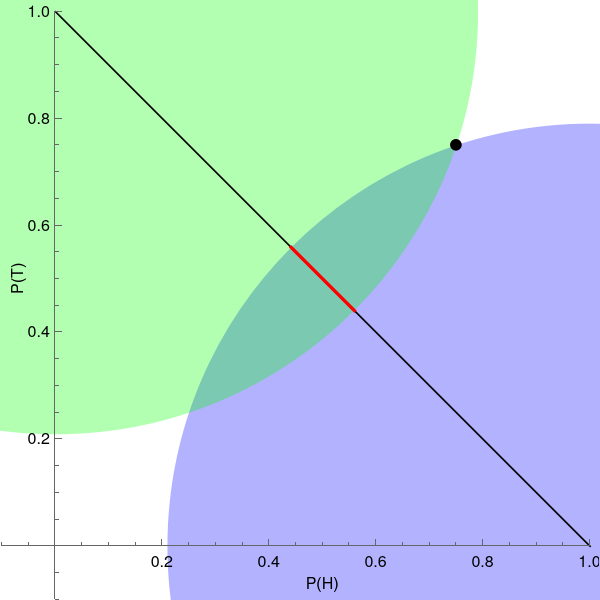
\includegraphics[width=0.7\textwidth]{Scoring rule graph.png}
\medskip
\caption{An illustration of the accuracy argument for a simple two-event $\Omega$}
\label{f:scoringrule}
\end{figure}

The claim of the scoring rule argument is that there is another probability assignment that will do better no matter what the world is.  So, what are they?  

First, let's consider what happens if the coin comes up Heads.  In that case the ideal probability assignment is the point in the lower right corner, where $P(H) = 1$ and $P(T) = 0$.  So in that world, Mandy would prefer any probability assignment that is closer to that corner to the one she currently has.  All these are illustrated by the blue circle which is centered on the point in the lower right corner.

But that's just for one possible state of the world?  What about the other?  What if the coin had come up Tails?  Now the ideal probability distribution is one where $P(H) = 0$ and $P(T) = 1$, the point in the upper left corner of our graph.  Now Mandy would prefer any probability assignment which lies within the green circle that is centered in the upper left.

Notice something about our circles: there is a lens shaped region where the two circles overlap.  Any probability assignment that lies in that region will do better {\it no matter what the state of the world is}.  Of particular interest is the part of the black line that is highlighted in red.  Those are probability assignments which are consistent with the axioms and do better than Mandy no matter what is the state of the world.

What we've shown so far is that Mandy would do better to choose any point within the lens, which includes some points that are consistent with the axioms (but also some points that are not).  What if Mandy decided to choose a point in the lens, but one that is off the line---one that is not consistent with the axioms?

We could run the same argument again (and again) until she eventually chooses a point that lies on the line. Once there, no lens-shaped region exists.  The two circles will intersect at only one point, the point that represents Mandy's probabilities.  And this fact is our theorem.  If Mandy chooses any point off the line, then there will be a lens-shaped region where she could have done better no matter what.  If Mandy chooses any point on the line, then there will not be such a region. 

Before leaving this discussion, I should take a moment to talk about why we choose the Brier score as opposed to any other way of measuring distance.  There is a long (and sometimes complicated) literature about what conditions we might want a measure of ``inaccuracy'' to obey. Many scholars argue that any inaccuracy score should be whats called a {\it proper} scoring rule.  A proper scoring rule is one that is ``self endorsing'' that is the score always regards itself as most accurate {\it when it obeys the axioms}.  Brier score is one such rule but there are others.  Space will prevent a discussion of these reasons, but interested students should look more into the literature.

\section{Descriptive concerns}

\marginnote{This study is reported in \fullcite{rottenstreich1997}.}

In a famous experiment on probability estimation, a group of US undergraduate students where asked a series of questions about the probabilities of outcomes in the next presidential election.  We can think of the underlying space as being divided into three atomic events, which we assume are exhaustive. $D$: A democrat wins the election. $R$: A republican wins the election. And $I$: an Independent (defined as neither a democrat or a republican) wins the election.  In this case $\Omega = \{D, R, I\}$. From this we might construct an additional event (so that we can test the finite activity axiom).  That event is the event $N$: ``the person who wins is not a democrat'' or $N = \{R, I\}$.

The students were divided into several groups.  Some asked to evaluate the probability of $R$, some others the probability of $I$, and some others the probability of $N$.  It turns out that in this experiment the average estimates where $P(R) = 0.59$, $P(I) = 0.05$, and $P(N) = 0.6$.  This obviously violates the axiom of additivity (assuming that we treat each group like a single individual).

The hypothesis put forward is that presentation matters. When people are asked ``will someone who is not a democrat win?'' They think of the most likely alternative, in this case a republican.  This is why $P(N) \approx P(R)$.  They forget to include the probability of an unlikely, but possible, alternative.


Another example requires just a tiny bit more work, but is regarded as more definitive.  I will give you the original example, although at this point it feels dated.  (The original is from the early 1980s.)  Subject where asked to read this brief description of ``Linda'' 

\marginnote{This study is reported in \fullcite{tversky1983}.}

\begin{quote}
Linda is 31 years old, single, outspoken and very bright. She majored in philosophy. As a student, she was deeply concerned with issues of discrimination and social justice, and also participated in anti-nuclear demonstrations.
\end{quote}

They were then asked to rank order a series of statements by how likely they were:

\begin{enumerate}
\item Linda is a teacher in elementary school. 
\item Linda works in a bookstore and takes Yoga classes. 
\item Linda is active in the feminist movement. 
\item Linda is a psychiatric social worker. 
\item Linda is a member of the League of Women Voters. 
\item Linda is a bank teller. (We will call this: $T$) 
\item Linda is an insurance salesperson. 
\item Linda is a bank teller and is active in the feminist movement. (We will call this: $A$)
\end{enumerate}

Of particular interest to the experimenters were the labeled sentences ($T$ and $A$; the labels are for our purposes and were not shown to the subjects).  They found that 85\% of their subjects ranked $A$ as more likely than $T$.  Which is impossible. 

How does this violate additivity? Here we need to be a little careful.  When defining our universe of possibilities we need to think of all the relevant ones.  If we are just concerned with whether Linda is a bank teller (or not) and whether she is a feminist (or not), then we have to consider four possibilities: 

\begin{itemize}
\item[$A$:] Linda is a feminist and a bank teller
\item[$B$:] Linda is a feminist but not a bank teller
\item[$C$:] Linda is not a feminist but is a bank teller
\item[$D$:] Linda is neither a feminist nor a bank teller
\end{itemize}

So our universe, $\Omega = \{A, B, C, D\}$.  And now we can define an event ``Linda is a bank teller'', $T = \{A, C\}$. Finite additivity requires that $P(T) = P(A) + P(C)$.  So if people say that $P(A) > P(T)$, then they are {\it either} violating finite additivity {\it or} they think that $P(C)$ is negative.  The experimenters (and me) think it's more likely that they are violating additivity than they think probabilities can be negative.  

\section{Conclusion}

This chapter has introduced probability as the way to think about uncertainty. We introduced different interpretations of probability and discussed why the axioms might be regarded as normatively compelling under those different interpretations. We concluded with two short examples that suggest that people don't always obey the axioms when evaluating the likelihood of events.

To make our lives simple, I have tended to focus on easy to understand examples (like with dice).  One might think that the axioms are (descriptively or normatively) correct for simple things that like, but be skeptical in more complex cases. Do I need to obey the axioms when evaluating the probability that Linda is a bank teller? Or that there will be a war in the next decade? Or that intelligent life exists on another planet? Etc.

Other theories with both normative and descriptive interpretations have been developed to deal with different cases.  If you're interested, I would encourage you to follow up.

\chapter{Probability over time}

When we discussed the theory of preferences in chapter~\ref{c:certainty}, we pointed out that the theory is {\it synchronic}; it's only about consistency at a given time.  One needs to obey the axioms today. One also needs to obey them tomorrow (and the next day, and the next).  But the axioms don't tell you how today relates to tomorrow. It doesn't tell you anything about preference change.  It doesn't violate the axioms that I switched my preference between candy and salad sometime in the last 40 years.

So far, the subjectivist theory of probability is the same.  It tells you how today-beliefs ought to cohere with other today-beliefs. It tells you how tomorrow-beliefs ought to cohere with other tomorrow-beliefs. What we have not yet discussed is how today-beliefs need to cohere with tomorrow-beliefs.

That might seem very strange thing to say, and you might find it perplexing.  So let's start with an example of what I mean.

Suppose that today Mandy's subjective probability in the event ``we'll find life on Mars'' is 0.6.  Suppose that Mandy dutifully obeys the probability axioms in all her beliefs, so she not subject to a book or distance argument.

Today Mandy forms a plan: When she wakes up tomorrow, her new probability for finding life on Mars is going to be 0.2. She doesn't think she's going to learn anything that is relevant to the question of life on Mars. She just wants to ``keep people on their toes.'' She plans to adjust all her other beliefs tomorrow to ensure that she is consistent with the probability axioms accordingly. She doesn't want to be irrational, after all.

Has Mandy done anything wrong? Is her plan rational?  If she follows through, would we think that was okay?  It sure seems weird.  Rationality, one might argue, should require you to only change your beliefs in response to learning something relevant.  Mandy is obeying the axioms, but is violating this other intuitive constraint.

\section{Conditional probability and Bayes theorem}

We didn't introduce it in the last chapter,  there is a type of probability called ``conditional probability.''  Often it is denoted with the symbol: $|$.  So, you would read: $P(F | E)$ as ``the probability of event $F$ conditional on $E$.'' In probability textbooks it is defined this way:
\begin{equation}
    \label{e:conditional-prob}
    P(F | E) = \frac{P(F \cap E)}{P(E)}
\end{equation}

\nomenclature{$|$}{Conditional probability. $P(E|F)$ is read as ``the probability of $E$ conditional on $F$.''}
\nomenclature{$\cap$}{Set theoretic intersection. $X \cap Y$ is the set which contains elements that are in both $X$ and $Y$ and no others.}

While conditional probability can mean many things, one common way of interpreting it is that it is the probability of $F$ after learning that $E$ happened.  This definition of conditional probability gives rise to the most famous equation in probability: {\it Bayes Theorem}. 

To understand Bayes' theorem, let's start with a simple example.  Suppose that Frick Honeydew University is developing their academic integrity policy.  FHU thinks that there are two basic types of students, those who are irredeemable cheaters and those who are not. It wants to know: when we catch a student cheating, how likely is it that this student is an irredeemable cheater versus a student who just made a stupid mistake?  It conducts a study of its students and faculty and estimates the following probabilities.

\marginnote{{\bf Please note}: these numbers are completely made up for the purposes of this example. They don't represent any real data about anything.} Most students are not irredeemable cheaters (event $I$), so the $P(I) = 0.05$. The probability that a an irredeemable cheater is caught cheating one time in their career (event $C$) is high, $P(C|I) = 0.8$. Good students make mistakes and cheat, even though they aren't irredeemable.  So, $P(C|\neg I) = 0.1$

\nomenclature{$\neg$}{Negation or set theoretic inverse. $\neg E$ means all the events in $\Omega$ which are not in $E$.}

Now FHU wants to know, when we catch a student cheating for the first time, what is the probability that they are an irredeemable cheater?  Notice we don't yet have that information. We know that {\it if} the student is irredeemable, then the probability that they will be caught is 0.9.  But what FHU wants to know is different. FHU wants to know {\it if} the student is caught, what the probability that they are irredeemable?

If you are struggling a bit with the difference between these two, consider this analogy.  Suppose that I choose a person currently living on Earth at random.  I know who they are, but you don't.  I decide to convey a little information to you: They live in the US.  What is the probability that they speak English?\marginnote{These numbers about English speakers are not made up by me, they come from Wikipedia.} As of 2022, it was about 90\%. It's not surprising that the vast majority of people who live in the US speak English. 

Now, suppose that I choose another person who llives on Earth at random. I tell you: They speak English.  What is the chance they live in the US? Now the number is much lower.  Why is it lower? There are many reasons.  First, English is the main language of several other countries (like the UK). Also, many countries have significant English-speaking populations (like India). And finally, English is becoming a very common second language for the global population.  The chance that a random English-speaking person lives in the US is more like 20\%. 

This shows the difference between the two conditional probabilities. The probability of speaking English conditional on living in the US and the probability of living in the US conditional on speaking English.

Now, we return to our example of Frick Honeydew University. FHU knows one direction: the probability that someone gets caught cheating conditional on being irredeemably a cheater (and not being that).  They want to know the opposite: the probability of being irredeemably a cheater given that they were caught cheating.  What should they do?  This is where Bayes' theorem comes in.

First let's list what we know:
\begin{align*}
    P(I) & = 0.05\\
    P(\neg I) &= 0.95\\
    P(C|I)  & = 0.8\\
    P(C| \neg I) &= 0.1
\end{align*}

What we want to know is $P(I|C)$.  So let's see if we can come up with an equation that gives us this number.  We'll start with the definition of conditional probability:
\begin{equation}
\label{e:igivenc}
P(I|C) = \frac{P(C \cap I)}{P(C)}
\end{equation}
Unfortunately, we don't know either of the terms on the right hand side.  But perhaps we can transform them as well.  First, let's focus on $P(C \cap I)$. Let's start with a different conditional probability:
\begin{equation*}
P(C|I) = \frac{P(I \cap C)}{P(I)}
\end{equation*}
By multiplying both sides, this gives us
\begin{equation}
\label{e:multirule}
P(I \cap C) = P(C|I)P(I)
\end{equation}
We know both of the terms on the right hand side. Notice that $I \cap C = C \cap I$, so we also write this as: $P(C \cap I) = P(C|I)P(I)$.  This helps some. If we substitute this into equation~\ref{e:igivenc} we get:
\begin{equation}
\label{e:bayeshalf}
P(I|C) = \frac{P(C|I)P(I)}{P(C)}
\end{equation}

We're part way there. Now how do we deal with the denominator, $P(C)$? The first trick is to recognize that the event $C$ can be expressed as two mutually exclusive events: $C \cap I$ and $C \cap \neg I$.  (The basic idea is that you can separate $C$ into the parts it shares with $I$ and the parts that it doesn't.)  So now we have $C = (C \cap I) \cup (C \cap \neg I)$. Since these are mutually exclusive:
\begin{equation*}
P(C) = P(C \cap I) + P(C \cap \neg I).
\end{equation*}
We can do the same trick we did with equation~\ref{e:multirule} and rewrite this as:
\begin{equation}
\label{e:lawoftotalprob}
P(C) = P(C|I)P(I) + P(C|\neg I)P(\neg I)
\end{equation}
This equation is sometimes called {\it the law of total probability}. Its interpretation makes sense: I can reason by cases. If I want to know what is the chance that someone is caught cheating (or anything else), I can break it into two parts. What is the chance they are caught cheating if $I$ happens and what is the chance if $I$ doesn't happen. We have to weigh these two by their respective probabilities.

With the law of total probability in hand, we can substitute it into equation~\ref{e:bayeshalf} and get:
\begin{equation}
\label{e:bayesthm}
P(I|C) = \frac{P(C|I)P(I)}{P(C|I)P(I) + P(C|\neg I)P(\neg I)}
\end{equation}
This is known as Bayes' theorem. It solves FHU's problem.  The left-hand side is what the University wants to know, and it already knows all the terms on the right-hand side. 

When we substitute all known probabilities, we end up with $P(I|C) \approx 0.3$.  Although being caught is evidence of someone being an irredeemable cheater, it is definitely not a guarantee.  Why?  Because irredeemable cheaters are rare, even if you see strong evidence that someone is one, in many cases you might want to wait for more evidence.

\nomenclature{$\approx$}{Numerically approximately equal to. Importantly distinct from $\sim$ and $=$.}

This point is very critical and underlies a huge number of fallacious inferences we find in every day life.  The mistake of ignoring the rarity of things is called {\it base rate neglect}. For example, vaccine skeptics noted that most people hospitalized for COVID had received one of the COVID vaccines. Is that evidence that the vaccine is ineffective? No! As long as a sufficiently large fraction of the population received the vaccine (which is the case), we would expect that statistic even if the vaccine is incredibly effective.  Examples abound.

Bayes' Theorem and variations have been incredibly influential.  It inspired a whole area of statistics known as Bayesian statistics. Much of economics is built on Bayes' Theorem. Philosophers have argued that Bayes' Theorem is fundamental to understanding how scientific reasoning works. And Bayesian theories in psychology are one popular way to model the mind.

\section{The principle of conditionalization}

Bayes theorem, as powerful as it is, remains fundamentally synchronic. It tells you what to assign to one conditional probability given what you assign to others.  Let's return to the story of Mandy with which we began.  Recall that all of Mandy's probabilities are consistent with all the axioms.  She even has conditional probabilities, and she obeys Bayes' Theorem when assigning them. But she doesn't always change her probabilities in accordance with conditional probabilities.  Sometimes she changes them even though she's learned nothing relevant.  What's wrong with what she does?

Mandy violates this principle:
\begin{quote}
{\bf Principle of planned conditionalization} If an agent's subjective beliefs at some time $t$ are represented by $P(x)$, then their plan for their future probability function at some later time $t^\prime$ should be represented by $P^\prime(x) = P(x|E)$, where $E$ represents the event which contains {\it all and only} those things they learned in between $t$ and $t^\prime$.  
\end{quote}
Mandy violates the principle of conditionalization when she anticipates changing her probability function despite learning nothing relevant.

Why exactly does Mandy violate this principle?  If Mandy learns nothing, we can treat it as if she learned $\Omega$. Recall that $\Omega$ is sometimes called ``the sure event'' that is guaranteed to occur. So learning that ``something will happen'' gives you no information.  The principle of conditionalization requires that Mandy's probabilities tomorrow be $P^\prime(x) = P(x|\Omega)$ and $P(x|\Omega) = P(x)$.  So the principle of conditionalization requires that you not change your probabilities when you don't learn anything that you think is relevant.

That's one way of violating the principle: changing even though you didn't learn anything.  A different way of violating the principle of conditionalization involves {\it not} updating when you {\it do} learn something.  Imagine the following conversation:
\begin{dialogue}
    \speak{Aydin} I don't think John Q. Politician will win the election.  If he supported the expansion of healthcare coverage, I think he would win.  But since he doesn't, I don't think he has much of a chance.
    \speak{Esha} Oh, you didn't hear?  John Q. Politician just came out with a public statement declaring that he does, in fact, support the expansion of healthcare coverage.
    \speak{Aydin} I didn't know that.  I still don't think he's going to win.
\end{dialogue}

In this exchange, Aydin has violated the other half of the principle of conditionalization. He didn't update his probability as he promised he would when he received new information.

These two violations involve updating having learned no information or not updating on having learned relevant information.  One might violate it a third way by updating, but in a different way than you had planned.

Consider one last dialog

\begin{dialogue}
    \speak{Toby} I don't think the AFLW Collingwood Magpies are going to make the final series this year.  I'd give it 10\%.  But if they {\it do} make the final series, I think they are about equally likely to win or lose the championship.
    \speak{Janine} Oh, you didn't hear! The season is already over, and the  Magpies made the final series!
    \speak{Toby} I didn't know that. I'm still feeling pessimistic, though.  The Magpies always find a way to screw things up. I think the chance they win the championship is 25\%
\end{dialogue}

Although Toby did update his probabilities, he did so in a different way than he committed to.  At first, he claimed he would assign the probability 50\% but then he actually assigned it 25\%.

\section{Arguments for the principle of conditionalization}

While all these violations seem irrational, we might ask {\it why} they are irrational?  What exactly is wrong with what Mandy, Aydin, and Toby are doing?  Like with synchronic constraints, there are the same two basic strategies: a book argument and an accuracy argument.

Why should one follow the principle of conditionalization?  There are two classic arguments that both follow the same format as before.  One involving books and one involving accuracy. 

\subsection{Diachronic book arguments}

We'll start with the book argument. Although we will not dive into the full proof of the diachronic book argument, we will give two illustrations.

We will keep the same story as with the earlier book arguments.  Mandy must post prices for tickets that correspond to every event in $\mathscr{P}(\Omega)$. She must be willing to buy and sell tickets at that price.  We will add one additional thing: the Bookie and Mandy will interact twice. They will interact before and after some event (like interact today and tomorrow).  If the bookie has a strategy whereby he can guarantee a win from Mandy including all his bets from both today and tomorrow, then we will say that Mandy has been subject to a {\it diachronic book}. 

First, let's start with Mandy's plan to change her probability in the event ``we'll find life on Mars'' from 0.6 today to 0.2 tomorrow despite learning nothing of relevance.  Our bookie can now form a very simple plan.  Today he'll sell a ticket to Mandy that pays \$1 if we find life on Mars for the price of \$0.60.  Mandy will pay for it.  Tomorrow, he offers to buy that same ticket back from her for \$0.20, which she will also take.  In the end, the bookie sold high and bought low, he made \$0.40 and is at no risk of losing money. 

Now, let's consider the story of Toby, the cautious sports fan. He always finds reasons to be overly skeptical of her team's chances.  Recall, Toby thought the chance of the Magpies making the final series (call this event $F$) was low $P(F) = 0.1$. But he said that if the Magpies make it to the final series, then the chance they win the championship is $0.5$ (call this event $C$). His current probability is $P(C|F) = 0.5$.  We will assume that his today-probabilities, $P$, obey all the axioms of probability. Thus, we know that Toby cannot be booked using only bets with his probabilities {\it today}.

Let's suppose that Toby can predict his pessimism. Even before Janine tells him the season is over, he can predict that he will become skeptical as a self-protection mechanism. He will then assign $P^\prime(C) = 0.25$.  Of course, if the Magpies don't make the final series, he knows they cannot win the championship and he will assign the correct probability.

This is a violation of the principle of conditionalization.  What we will now show is that a Bookie can make a series of bets with Toby that make him guaranteed to lose. 

The Bookie will visit Toby before the season ends and buy and sell tickets.  Then after the season ends and Toby learns whether Magpies make the final series (event $F$) the Bookie will return and will have the opportunity to buy and sell tickets with Toby again.

I've already said that the Bookie can subject Toby to a book, so let's see what it is.  Recall that Toby's probabilities before the end of the season obey the axioms of probability, so we can calculate the price he will post on the ticket $P(C \cap F) = 0.05$.\marginnote{As an exercise, make sure that you agree that $P(C \cap F) = 0.05$ for Toby.}  The bookie will, today, make the following exchanges with Toby:
\begin{itemize}
    \item {\it Exchange 1}: Sell Toby {\it four} tickets on the event $C \cap F$ for \$0.05 each
    \item {\it Exchange 2}: Sell Toby {\it one} ticket on the event $\neg F$ for \$0.90.
\end{itemize}
So far, there is no book here.  Toby might win money (if, for example, $C \cap F$ occurs). That is expected since Toby obeys the axioms of probability before the season ends. Now we have to add what the bookie will do after both Toby and the Bookie learn whether $F$ happens:
\begin{itemize}
    \item If $F$ happens, {\it Exchange 3}: Buy from Toby {\it four} tickets on the event $C$ for \$0.25 each
    \item If $\neg F$ happens, do nothing
\end{itemize}

The results for this bet are pictured in this table:
\begin{table}[h!]
\centering
\begin{tabular}{ccccc}
\toprule
Event             & Exchange 1 & Exchange 2  & Exchange 3 & Total \\
\midrule
Not-$F$           & -0.20       & 1 - 0.90   & 0          & -0.10 \\
$F$, Not-$C$      & -0.20       & -0.90        & 1         & -0.10 \\
$F$ and $C$       & 4 - 0.20  & -0.90        & 1-4      & -0.10\\
\bottomrule
\end{tabular}
\medskip
\caption{A diachronic book from the perspective of Toby's payoffs.}
\end{table}

You can see that no matter what happens, Bookie will make money (and Toby will lose it).  

The more general form of the book is a bit more complicated, and we will not go into the full details. Suffice it to say that this can be extended to any violation of the principle of conditionalization.

\subsection{Diachronic accuracy arguments}

To illustrate the accuracy version of this argument, we will again focus on the story of Toby.  Recall that today, Toby has the following probabilities:
\begin{align*}
    P(F) & = 0.1\\
    P(C|F) & = 0.5\\
    P(C|\neg F) & = 0 \\
\end{align*}

Let's consider two different ``updating strategies'' that Toby might follow.

{\bf Strategy 1:} Toby will stick to his original plan.  If the Magpies make the finals series, then he will in fact assign the probability of them winning the championship 50\%.  That is, Toby plans to adopt the following probability if the Magpies make the final series:
\begin{align*}
    P_F^1(C) & = 0.5\\
    P_F^1(\neg C) & = 0.5\\
\end{align*}
If the Magpies don't make the final series, he will do the obvious thing:
\begin{align*}
    P_{\neg F}^1(C) & = 0\\
    P_{\neg F}^1(\neg C) & = 1.0\\
\end{align*}

{\bf Strategy 2:} Toby will do the pessimistic thing that he is inclined to do
\begin{align*}
    P_F^2(C) & = 0.25\\
    P_F^2(\neg C) & = 0.75\\
    P_{\neg F}^2(C) & = 0\\
    P_{\neg F}^2(\neg C) & = 1.0\\
\end{align*}

The question we are asking now is which strategy should Toby prefer today.  Recall from section~\ref{s:synchronic-accuracy}, that one version of accuracy argument makes use of a measure of inaccuracy called the Brier score. 

We can ask a question of Toby today (before he learns that whether the Magpies make the final series). Which strategy do you think, Toby, will be more accurate on average?

To do this we have to think of several possibilities.  If the Magpies don't make the final series, then Toby thinks that both strategies are equally accurate.  So, we can ignore that part.  If the Magpies do make the final series, and if they do win the championship, then strategy one will have a distance to the truth of $(1-0.5)^2 = 0.25$.  While strategy 2 will have a distance to the truth of $(1-0.25)^2 = 0.5625$.  So IF the Magpies win, then he would prefer strategy 1 to strategy 2.

But of course, if the Magpies don't win, he would prefer strategy 2 to strategy 1.  If they don't win, then strategy 1 again gives him a distance of $(0-0.5)^2 = 0.25$.  But strategy 2 gives him a distance of $(0-0.25)^2 = 0.0625$. So strategy 2 is better.

How shall Toby choose?  Well he can calculate how the two strategies will do on average (we'll return to talking about this way of deciding in chapters~\ref{c:vnm} and~\ref{c:aa}).  Assuming that the Magpies make the final series, {\it today} Toby thinks their probability of winning the championship is 0.5.  So, the average of strategy 1 will be 0.25.  The average of strategy 2 will be 0.3125.  So, on average strategy 1 will be closer to the truth than strategy 2.

Like with the book argument, this can be expanded to include any violation of the principle of planned conditionalization. But, we won't dive into all those details here.
    
\section{Normative concerns}

It's fair to say that the principle of conditionalization is somewhat controversial.  Although many people in the sciences (especially statistics and economics) use the principle without any defense, some scholars are skeptical. There is a large debate about various objections and concerns. We could not possibly hope to exhaust them here, but I will try to give you a taste of some of them.

\subsection{The Problem of the Priors}

Imagine Mandy takes the principle of conditionalization quite seriously. At a young age, she forms an $\Omega$ over everything she expects to learn.  She sets up a giant spreadsheet and enters all her subjective probabilities.  Some of those probabilities might be based on solid reasons, like she assigns a probability of 0.5 to seeing heads on the flip of a coin.  Some of those probabilities might be pure guess work, like the chance that she will have exactly four grandchildren by the time she is 70. 

If Mandy is committed to the principle of conditionalization, in a sense she made all her decisions about her subjective beliefs when she created that spreadsheet. She listed all her conditional probabilities.  When she learns something that is in her spreadsheet, she just needs to update on that.  The rest of Mandy's beliefs for all of time are (relatively) simple computations.

To many, this feels like a kind of arbitrary tyranny of Mandy's earlier beliefs. Why should today's beliefs be shackled by what Mandy believed years and years ago?  This is especially true when we recognize that so many of our beliefs were formed on the basis of more or less arbitrary guesses.

\marginnote{For the details of the convergence to the truth theorems, see \fullcite{Shervish1990}.}
Defenders of the principle of conditionalization appeal to two mathematical claims to defend themselves against this charge. The first claim is often called the {\it convergence to the truth} theorems.  Without getting into too much detail, the basic idea is that as someone updates their probabilities using the principle of conditionalization and if they receive an unending stream of evidence, they will get closer and closer to the truth.  This requires a few assumptions, including that they don't initially assign the truth probability $0$ and a few others, which we will not go into here.

\marginnote{For details of the merging of opinions theorem, see \fullcite{blackwell1962}.}
The second mathematical claim is called {\it merging of opinions}. Merging of opinions is similar, but doesn't require a truth. Suppose that you have two people who obey the principle of conditionalization: Mandy and Teddy.  They initially assign probabilities to events, perhaps somewhat arbitrarily.  But suppose that they agree on this much: what counts as having probability zero.  In that case, eventually, with enough evidence, Mandy and Teddy will come to agree.  Whatever are their disagreements, they will {\it eventually} disappear.

\subsection{Surprising information}

Suppose that you actually tried to implement that giant spreadsheet. You might quickly run into a problem: you can't actually think of everything you might learn. Something might happen which is genuinely surprising: not because you assigned it zero probability, but because you literally did not think about it.  Call this event $Z$

If $Z$ happens, you cannot update with your conditional probabilities, because you don't have them.  As a result, the principle of planned conditionalization tells you nothing about what you should do.

The degree to which this is a concern depends on your perspective. Some people think this is a problem, because they want a theory of rationality that tells you what you ought to do in every logically-possible circumstance.  Other people feel like this is asking too much: this theory tells you what is rational when something predictable happens and is just silent about what to do when something unpredictable happens.

\marginnote{The problem of old evidence was first discussed in \fullcite{glymour1980}.}
One way that this concern might seem especially troubling is with a version of this story called {\it the problem of old evidence}. 

The problem of old evidence is inspired by an episode in the history of science.  It was known for a long time that Mercury's orbit was inconsistent with the best theory of gravity we had at the time: Newtonian mechanics.  No one understood why (although several theories were offered).  Along came Einstein, with a new theory of gravity that explained the orbit of Mercury.  

Why is this a problem? Well, the theory came after the evidence. It's not as if Newton had thought of Einstein's theory and the fact about Mercury's orbit and assigned conditional probabilities to those events.  He just hadn't thought of Einstein's theory: the creation of this theory was an unexpected event.

We can't just add Einstein's theory into our algebra and act like everything is fine, either.  Why not?  Because we already know that Mercury's orbit does what it does.  We can't update on that fact because it's old evidence: we already assign probability 1 to Mercury's orbit being what it is.  So, we can't add in Einstein's theory and update using Bayes theorem.

Perhaps we could do something more sophisticated an imagine what things would have been if we had first had Einstein's theory and then later discovered the important facts about Mercury's orbit. People debate about whether this is worth doing, or if its even feasible.

\subsection{Learning constraints}

There is another problem with thinking about the principle of planned conditionalization as a one-size-fits-all model for learning: it's not clear if everything you might learn can or should be thought of as an event in the sense of probabilities.  

\marginnote{The Judy Benjamin problem was first presented in \fullcite{vanfraassen1981}.}
A simple story is often used to illustrate this problem called the ``Judy Benjamin'' problem.  Judy Benjamin is a fighter pilot flying along the line between friend and foe. Something goes wrong with her plane and she has to eject. To make this situation simple, we might imagine that there are for quadrants and Judy Benjamin must figure out where she is.  Figure~\ref{f:judybenjamin} depicts the four possibilities.

\begin{marginfigure}
\centering
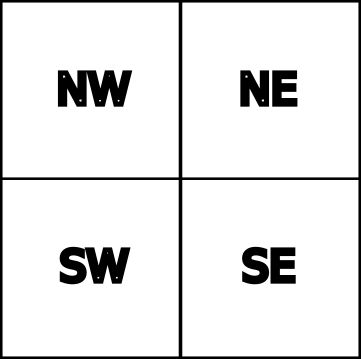
\includegraphics[width=\textwidth]{JudyBenjamin.png}
\caption{Where could Judy Benjamin be?}
\label{f:judybenjamin}
\end{marginfigure}

Initially Judy Benjamin thinks its equally likely she is in any of the quadrants.  Formally she think $P(NW) = P(NE) = P(SW) = P(SE) = \frac{1}{4}$.  Her radio is badly damaged, and just as it is failing she hears an important piece of information from her headquarters:
\begin{quote}
{\it If} you are in the North, we think it's three times more likely that you are in the west.  
\end{quote}
Then the radio fails.

Why this is this a problem? It seems like Judy Benjamin has just learned an important piece of information. She has learned that, whatever her probabilities are it needs to be that $P(NW) = 3 P(NE)$. In fact, it seems quite natural to a lot of people that she should hold fixed $P(SE)$ and $P(SW)$ since she hasn't learned anything about them.  And instead she should adjust $P(NW) = \frac{3}{8}$ and $P(NE) = \frac{1}{8}$.

Unfortunately, Bayes theorem cannot explain our intuitions about this case.  The problem arises because there is no event which corresponds to the radio transmission. Judy Benjamin learned the relationship between two probabilities (or, perhaps, a conditional probability).  But those aren't events.

There are a couple of ways to try and deal with this problem.  One is to adopt other forms of updating that allow for learning arbitrary mathematical constraints. Another is to explicitly expand the set of atomic events so that Judy Benjamin can handle different transmissions from headquarters as events themselves. 

\subsection{Some sentences aren't events}

When I first learned about probability and Bayes theorem, I got really excited about the power to handle uncertainty.  I started thinking about how to apply probability to a large array of different problems.  But, I discovered that it's difficult to always construct the mathematical representation of an event space for every possible sentence.

Take, for example, the sentence ``today is Tuesday.'' This sentence cannot be a simple event in a probability space.  Why not? Well if you assign it probability 1 today, then it had better be probability 0 tomorrow. Then in seven days it will again have probability 1.  Etc.  This cannot be handled by the principle of conditionalization.

There are attempts to expand probability to deal with a broader set of natural language sentences, but it does require work in order to be able to do that.  And of course, the principle of conditionalization will no longer hold in full generality.  Bayes theorem doesn't allow you to go from probability 1 to 0, but that's exactly what I do when I wake up the day after Tuesday.

\section{Conclusion}

There are actually many more potential counter examples to the principle of conditionalization. Philosophers will likely continue to debate it for decades.  I could not hope to give you a full picture of the debate, but here is a taste. If you are interested in learning more, there are many books that go into many more details.

You might have also noted this chapter doesn't have a section on descriptive concerns with the principle of conditionalization.  That in part because it's so difficult to determine if people obey it because, among other things, its difficult to know what people's conditional probabilities are.  Some psychologists think the mind obeys the principle of conditionalization (without us being conscious of it). They think that much about our psychology, like visual illusions and the like, can be explained by our brain updating with Bayes theorem. But there is a debate.

This chapter is a bit of an aside to the rest of the book.  For the remaining chapters, we will return to the comfortable world of the synchronic.  In particular, we will go back to a question we first raised way back in chapter~\ref{c:uncertainty-noprob}, how do we handle uncertainty.  If this book were longer, we could talk about decisions that take place over time, and we could combine this chapter with the next ones.  Alas, it isn't longer (agree with me here\dots please).  So, we won't be able to connect back.

\chapter[von Neumann\breakslash Morgenstern]{von~Neumann and Morgenstern Decision Theory}
\label{c:vnm}


%I think it would be good to add one "counterexample" example.  Like lexicography, minimax or something like that.  This will help to illustrate how one thinks about counterexamples.


So far, we've developed the theory of decisions under certainty in chapter~\ref{c:certainty}.  There we discussed how an agent might make choices when faced with outcomes where they know what will occur.  In chapter~\ref{c:probability}, we discussed how an agent should think about uncertainty.  We illustrated several popular arguments for why agents should think about uncertainty by assigning subjective probability judgments to those things about which they are uncertain.  We have just one piece of the puzzle left: how should agents make decisions when they are uncertain?

Take the example of dice.  Suppose Mandy is offered a very simple gamble, one that will pay \$10 if the dice lands \dice{1}, and \$0 if it lands any other number. Mandy is given the choice: she can take this gamble or she can have \$1 for sure.  Suppose that she chooses \$1 for sure.  Was that rational for her? Suppose that she later confronts a similar gamble that pays \$9 if the dice lands \dice{2} or \$1 for sure, and now she chooses the dice roll. Are both those decisions rational?  Or are they inconsistent with one another?

A natural way to think about this problem is to calculate the {\it expected monetary return}, that is to ask how much money Mandy would win on average if she took the gamble many times.  In that case, she should accept both gambles.  The first will pay on average \$10/6 (assuming we think this is a fair dice) and the second will pay \$9/6.  Both of these are larger than \$1.  

However, some agents may not value money in that way.  If Mandy has already promised to give that dollar to a friend who needs it to buy lunch, she might opt to refuse both gambles.  We want theory that allows Mandy to care about money in different ways, otherwise the theory will be far too restrictive.  If you are like me, however, you probably still think Mandy refusing the first gamble but accepting the second seems\dots well\dots strange.

Not only do we want to be a little more lax in our judgments about how money is valued, we also want a theory that can handle more than just money.  If Mandy is deciding whether or not to take an umbrella with her on her walk to work, she is still gambling but not with money.  Her gamble now involves outcomes like, ``get wet on the walk'' and ``needlessly take an umbrella'' and the like.  It's not at all clear how one might calculate an average of objects like this.

We need to develop some set of constraints for how Mandy makes decisions in the context of risk that isn't too constraining, but also does just say ``anything goes.''  This is what we will do in the next section.

\section{An outline of the strategy}
\label{s:vnm-strategy}

This book is not a novel, so I will give away the ending.  What we are ultimately trying to do is something like the strategy of {\it expected monetary return}, except with utility rather than money. The problem that we confronted in chapter~\ref{c:certainty} was that ordinal utility can't use averages.  We need a richer notion of utility which will allow averages. Then we can articulate a constraint on rational behavior: a rational agent must choose the gamble that maximizes expected utility.

This is a somewhat complicated process.  Let me give you a simple example first, then we will show how this simple example can be expanded. 

Let's start with a very simple case of decision under certainty. Suppose that Mandy is confronted with three beverage options for her regular afternoon drink with a colleague.  Mandy can order from among this set $X = \{$tea, coffee, soda$\}$.  Suppose that Mandy obeys all the relevant axioms we discussed in chapter~\ref{c:certainty}, so we can represent her as having a preference relation which is complete and transitive over the set.  Suppose her preferences look like this: tea $\succ$ soda $\succ$ coffee.  So we know that if tea is available, Mandy will order that.  If it's not she'll order soda. And if neither of those are possible, she'll make due with coffee.

As we mentioned in chapter~\ref{c:certainty}, the definition of $\succsim$ allow us to assign numbers to each outcome that represent Mandy's preferences.  Recall definition~\ref{d:util-representation}, which defines what we mean by ``represents'' in this context. 

Now suppose that Mandy's colleague Teddy loves to make bets, and loves to offer his colleagues like Mandy strange decisions.  Teddy offers to go buy Mandy a drink.  But, he only gives her two options.  Either ($A$) he will buy her a soda or ($B$) he will flip a (fair) coin and if it comes up heads buy her a tea and buy her a coffee if it comes up tails.  
Intuitively what do we think Mandy will do?  It seems like there isn't yet a clear answer to this question, since we don't really know anything about the {\it strength} of her preference.  How much more does she like tea than soda?  How much does she dislike coffee?  

If Mandy really (really) liked tea and regarded soda and coffee as nearly equivalent, it seems natural that Mandy might take the bet.  If she loses, she doesn't lose that much and if she wins, then she wins big.  But, if her preferences are different and she thinks that tea and soda a nearly the same, with coffee as a distant third, then she might opt for the sure thing of soda.

One way to measure this strength is for Teddy to experiment with different coins.  Suppose, instead of a fair coin, Teddy brings his collection of biased coins each day.  And each day he tries out a new one to see what Mandy prefers.  For some coins she chooses the uncertain gamble, other times she opts for a soda.  Eventually after experimenting for a while, Teddy finds a magic probability $\hat{p}$.  If Teddy offers her a gamble that gives her a tea with probability $\hat{p}$ and a coffee with probability $(1-\hat{p})$, then Mandy is indifferent between that gamble and getting a soda for sure.

Let's suppose, for a moment, that after extensive investigation, Teddy comes to be confident that Mandy has the following choice procedure.  If Teddy offers her a gamble that gives her tea with probability $p$ and coffee with probability $(1-p)$, she will...
\begin{enumerate}
\item ... strictly prefer the gamble to getting a soda for sure when $p > \hat{p}$
\item ... strictly prefer getting a soda for sure to the gamble when $\hat{p} > p$
\item ... be indifferent between the gamble and a soda for sure when $p = \hat{p}$
\end{enumerate}
Given that Mandy follows this procedure, it seems somewhat reasonable to think that $\hat{p}$ can help us to figure out Mandy's strength of preference between tea, soda, and coffee.  

We will construct a utility function  $u: X \to \mathbb{R}$. We will start by assigning numbers to the two extreme outcomes, her favorite (tea) and her least favorite (coffee).    For our own convenience we will start by assigning $u($tea$) = 1$ and $u($coffee$) = 0$. (Why is it okay for use to do this arbitrarily?  We will come back to that later.)  Once we do that, we can now assign $u($soda$) = \hat{p}$. 

If we use this particular $u(\cdot)$, then we can say that Mandy behaves {\it as if} she is maximized the expected utility, where $u(\cdot)$ represents her utility.  To see why, let's go through each example above.
\begin{enumerate}
\item Suppose that $p > \hat{p}$.  The expected value of the gamble is given by $p u($tea$) + (1-p) u($coffee$)$.  Since $u($tea$)=1$ and $u($coffee$)=0$, this simplifies to $p$.  Since $p > \hat{p}$, and since $u($soda$)=\hat{p}$, Mandy's expected utility is higher with the gamble than with a soda for sure.
\item Suppose that $\hat{p} > p$.  The expected value of the gamble is still given by $p u($tea$) + (1-p) u($coffee$) = p$. Since $\hat{p} > p$, and since $u($soda$)=\hat{p}$, Mandy's expected utility is higher with soda for sure than with the gamble.
\item Finally when $\hat{p} = p$, the two have the same expected utility.  Therefore Mandy is indifferent.
\end{enumerate}

How might this strategy go wrong?  Let me count the ways.  First, Mandy might not ever be indifferent.  Suppose that Mandy decided that if the probability of tea was greater than or equal to 1/2, then she would prefer the gamble.  If it was less than 1/2, she would prefer the soda.  There would be no point where Mandy was indifferent, and this strategy wouldn't work. 

Or maybe Mandy declares ``I don't gamble.  I will always prefer the soda unless $p=1$.''  In that case, the gambling strategy would say that $u($tea$) = u($soda$) = 1$, which violates our assumption that Mandy strictly prefers tea to soda.

At the other extreme, Mandy might have more than one point where she was indifferent.  Suppose Mandy said, ``if $p > 3/4$ I will prefer the gamble.  If $p < 1/4$ I will prefer the soda.  And if $3/4 \geq p \geq 1/4$ I will be indifferent.'' Now there is no longer a unique value that we can assign to $u($soda$)$ (although we might be able to assign a range to it).  Even more radically Mandy might divide up the interval in many different strange ways that would make this strategy impossible.

So far we've imagined problems that might arise for just this simple comparison of one gamble to one certain outcome.  But our problems might get even more complex if we had more options.  Suppose that we introduce a fourth outcome, water.  Now, $X = \{$coffee, tea, water, soda$\}$.  And suppose Mandy exhibits the following preferences:
\begin{enumerate}
\item tea $\succ$ soda $\succ$ water $\succ$ coffee
\item The gamble that give tea with probability 3/4 and coffee with 1/4 $\sim$ soda
\item The gamble that gives tea with 7/8 and coffee with 1/8 $\sim$ water
\end{enumerate}
Even here we would run into problems. As we did before, let's set $u($tea$)=1$ and $u($coffee$)=0$. Preference 2 tells us that $u($soda$)=3/4$.  Preference 3 tells us that $u($water$)=7/8$.  But Preference 1 tells us that soda $\succ$ water. We have another inconsistency.

%^^^ This is inconsistent with independence.  Maybe come back and show why (or an excercise)

Given all these, we might ask: what constraints can we impose on Mandy's choices in order to ensure this strategy works?  Then, we can ask two different questions: do those constraints seem normatively reasonable (does it seem like Mandy {\it ought} to obey them)?  Of course, we might answer ``no.''  They might seem too strong (or even too weak). As a second question we might ask: do  people usually, in fact, obey them (whether or not they should)?  And we might come to different or similar conclusions.

\section{The von Neumann\breakslash Morgenstern axioms}

\marginnote{The theory is presented in their famous book \fullcite{VonNeumann1953}.}
The mathematician John von Neumann and the economist Oskar Morgenstern created a beautifully simple theory which does what we are looking for.  It was motivated by an area of philosophy and mathematics called ``measurement theory'' which focuses on how we can convert ``qualitative'' judgments into numbers.  And that's essentially what we are doing here: converting a qualitative judgment (``this is better than that'') into a number.  

As we've done before, we will start with a set $X$ which represents all the possible individual rewards that Mandy might get.  Unlike before, our agent won't be choosing anything in this set (at least, not exactly). Instead, this is often thought of as all the outcomes from all the possible gambles she might confront.  If we imagine Mandy is going to a casino and playing roulette, $X$ would include all the possible amounts of money she might win or lose.  If we are thinking about someone deciding whether to take an umbrella to work, this should include the possibilities of getting wet (or not) along with the benefits and costs of having an umbrella.   Examples abound.

While the theory is capable of handling $X$'s that are infinitely large, we would need some different mathematics.  So to keep the problems (relatively) simple, we will always assume that $X$ has only finitely many members. Of course, $X$ can be very, very large but still be finite. So this constraint isn't particularly serious for representing most every-day decisions.

Now we need to represent gambles.  A gamble will be defined as a probability distribution over the objects in $X$. That is, a gamble $g: X \to [0,1]$ such that:
\[\sum_{x \in X} g(x) = 1\]
We will then let $Q$ be the set of all gambles over $X$.

\nomenclature{$g, h, i$}{Used to denote arbitrary gambles, that is probability distributions over the prize space.}

\nomenclature{Q}{The set of all objective probability gambles over a specified finite prize space.}

Important members of $Q$ are the certain gambles that assign probability 1 to a single outcome in $X$.  We will often just write these as the outcome itself. So, strictly speaking ``coffee'' refers to the gamble which gives you ``coffee'' with probability 1.  This is a bit of a pedantic point, but worth keeping straight.

We will also need to think about what it means to combine gambles with one another. Often these are called {\it compound} gambles, although they might be nonetheless quite simple.  To understand what we mean, you might imagine that I am offering to flip a coin.  If the coin comes up heads I'll give you a lottery ticket. If it comes up tails, I'll give you one free spin of a roulette wheel.  This is a kind of compound gamble, where the ``prize'' from flipping the coin is itself another gamble.

We will invent an operation $\oplus$ which allows us to combine two gambles into a compound gamble. Suppose that $p$ is a number in $[0,1]$.  Then you can think of this object $p g \oplus (1-p) h$ as a gamble where I first flip a coin that has probability $p$ of coming up heads. If it comes up heads, you win gamble $g$.  If it comes up tails, you win gamble $h$. This is what we mean by a ``compound'' gamble. It's a gamble that pays in other gambles.

\nomenclature{$\oplus$}{Gamble addition/compounding. $0.75 g \oplus 0.25 h$ represents the gamble that pays $g$ with probability 0.75 and $h$ with probability 0.25. Importantly distinct from regular numerical addition $+$.}

Will we just keep adding layers and ever-multiplying compoundness of gambles?  No, in fact, what we are going to assume is that $pg \oplus (1-p)h$ actually picks out a different gamble already in $Q$. Stated more formally,  $p g \oplus (1-p) h$ picks out the gamble $r \in Q$ such that for every $x \in X$, $r(x) = p g(x) + (1-p) h(x) $.

We should stop here for a minute and talk about this.  For many mathematically minded folks, this seems quite trivial and obvious.  But hidden in the mathematical definition is a real assumption that might be neither normative required or descriptively accurate.  The assumption is sometimes called {\it the reduction of compound gambles}.  

The reduction of compound gambles requires that we treat complex gambles exactly the same as simpler ones.  For illustration, we might ask if you think these two gambles are identical (in the sense that any agent will---or should---treat them as the same):
\begin{enumerate}
\item Teddy offers Mandy the gamble where Teddy will go to the coffee shop and buy her a tea with probability 1/4, a soda with probability 1/2, and a coffee with probability 1/4.
\item Teddy offers Mandy the gamble where first Teddy will flip a fair coin. If it comes up heads, he'll give her a soda right away.  If not, he'll go to the coffee shop and flip the coin a second time.  Then if it comes up heads on the second flip, he'll buy her a tea. If not, he'll buy her a coffee.
\end{enumerate}
This might seem to you obviously the same.  Or maybe not.  We won't have much time to address this issue, but it is worth noting it since, in some contexts, people have advocated that this should or is not how people think about all compound gambles.  We will, however, proceed as if it is.

With this in hand, we will now suppose that Mandy has a preference relation $\succsim$ which is transitive and complete defined over $Q$ (the set of all gambles over $X$).  As you will recall from chapter~\ref{c:certainty}, we could also do this with choice functions where Mandy obeys Sen's $\alpha$ and $\beta$. 

This is our first axiom:
\begin{definition}[Axiom 1]
$\succsim$ is complete and transitive defined over $Q$.
\end{definition}

This inherits with it all the concerns that we laid out in chapter~\ref{c:certainty}. We won't rehearse them here, but they are not solved by moving to gambles.  $Q$ is now infinite, and contains objects which are arbitrarily close to one another.  So problems, like the concern about just noticeable differences, might be especially worrying in this context.

As we saw in previous section, this won't be enough. All the strange examples I showed you there could be expanded to be complete and transitive preferences over $Q$.  So we need to add two additional axioms which will, as we'll see in the next section, prevent those (and many other) preferences.

\begin{definition}[Axiom 2, Independence]
For all $g, h, i \in Q$ and all $p \in (0,1]$, if $g \succ h$ then $p g \oplus (1-p) i \succ p h \oplus (1-p) i$
\end{definition}
\nomenclature{$(], [)$}{Used to denote the half-open interval of numbers. For example (0,1] denotes the set of real numbers that are strictly greater than 0 and less than or equal to 1.} Before we talk about this axiom, please note the condition ``$p \in (0,1]$''  This is called a ``half open'' interval.  If you haven't seen it before, it is a compact way of saying $p$ is strictly greater than 0 and less than or equal to 1.

The independence axiom can be motivated by thinking (again) about numbers.  If two numbers $a$ and $b$ are such that $a > b$, then for any number $c$, $a + c > b + c$.  A similar thing is going on with independence, except the numbers are gambles and addition is replaced by gamble mixing, $\oplus$.  The comparison to numbers can make this seem less controversial than it is, however.  There are some interesting counter examples to this axiom, which we will discuss later in this chapter. 

Our last axiom eliminates many counterexamples that people often find plausible.  It prevents Mandy from adopting the attitude ``I don't gamble'' and preferring all certain options to uncertain ones.  It also prevents decision rules that only pay attention to the best- or worst-case outcomes (like maximin and maximax).  

\nomenclature{$()$}{Used to denote the open interval of numbers. For example (0,1) denotes the set of real numbers that are strictly greater than 0 and strictly less than 1.}

\begin{definition}[Axiom 3, Continuity]
For all $g, h, i \in Q$, if $g \succ h \succ i$ then there exists $p, q \in (0,1)$, where $p g \oplus (1-p) i \succ h \succ q g \oplus (1-q) i$
\end{definition}
Again note the ``open'' interval, which says that $p$ and $q$ are both greater than 0 and less than 1.

Like with Independence, thinking about numbers is helpful here.  Suppose three numbers $a > b > c$. There is some fraction $p \in (0,1)$ such that $p a + (1-p) c > b$.  Depending on how far apart $a$, $b$, and $c$ are, $p$ might be very large, but there will always be one.  The continuity axiom is saying the same for gambles.

What this axiom eliminates (among other things) is ``a bad thing so bad that you will avoid it no matter what.''  Suppose that gamble $i$ is sooo bad that you would sacrifice anything to avoid even a tiny probability of it.  In that case, although $g \succ h \succ i$, you would always prefer $h \succ p g \oplus (1-p) i$ for any $p<1$.  Continuity prevents you from feeling this way about anything.  It also prevents the symmetric case where you love something so much that you would give anything for even the tiniest chance of getting it.

It turns out that these three axioms are all you need to guarantee the strategy I described above will work.  Before proving that fact, though, I would like to take a moment to discuss one reason why the axioms are controversial. 

\section{The Allais paradox}

\marginnote{Allais originally published his paradox in French in:~\fullcite{allais1953}.} The paradox was suggested by Maurice Allais in the early 1950s.  Initially he proposed his paradox as a thought experiment, but there have since been many (many!) actual experiments to validate his concern.

Allais proposed that you consider two different choices between two different sets of gambles.  Here is choice 1. Before reading any further, take a moment and decide which of the two gambles you prefer or whether you are indifferent.

\begin{table}[h!]
\centering
\begin{tabular}{cccc}
    \toprule
    \multicolumn{2}{c}{Gamble $g_1$} & \multicolumn{2}{c}{Gamble $g_2$} \\
    {\bf Outcome} & {\bf Probability} & {\bf Outcome} & {\bf Probability} \\
    \cmidrule(lr){1-2}\cmidrule(lr){3-4}
    \$1 million & 1.0                 & \$5 million   & 0.10 \\
                &                     & \$1 million   & 0.89 \\
                &                     & \$0           & 0.01 \\
    \bottomrule
\end{tabular}
\medskip
\caption{Choice 1}
\end{table}

Choice 2 involves two different gambles. Again, take a second to think about which you might choose.

\begin{table}[h!]
\centering
\begin{tabular}{cccc}
    \toprule
    \multicolumn{2}{c}{Gamble $g_3$} & \multicolumn{2}{c}{Gamble $g_4$} \\
    {\bf Outcome} & {\bf Probability} & {\bf Outcome} & {\bf Probability} \\
    \cmidrule(lr){1-2}\cmidrule(lr){3-4}
    \$1 million & 0.11                & \$5 million   & 0.10 \\
    \$0         & 0.89                & \$0           & 0.90 \\
    \bottomrule
\end{tabular}
\medskip
\caption{Choice 2}
\end{table}

Many people (although not everyone) prefer $g_1 \succ g_2$ in Choice 1.  In Choice 2, gamble $g_4 \succ g_3$.  Although it is not obvious at all at first, this pair of choices is inconsistent with the the combination of Axiom 1 and 2 (Independence).  

We will demonstrate this formally in a moment, but you can get a sense for the problem with a simple illustration.  Imagine that the gambles are created using one of those giant lottery-ball machines.  There is a container with balls numbered 1-100.  Each ball corresponds to a prize in the different lotteries as follows:

\begin{figure}[h!]
\centering
    \begin{game}{4}{3}[][Number]
                & 1-10 & 11-99 & 100 \\
     Gamble $g_1$ & \$1 million & \$1 million & \$1 million \\
     Gamble $g_2$ & \$5 million & \$1 million & \$0  \\
     Gamble $g_3$ & \$1 million & \$0 & \$1 million \\
     Gamble $g_4$ & \$5 million & \$0 & \$0
    \end{game}
    \medskip
    \caption{A normal form representation of the four gambles}
\end{figure}

Notice something about these gambles.  If you ignore the middle column for a moment, Gambles $g_1$ and $g_3$ are identical and Gambles $g_3$ and $g_4$ are identical.  These pairs only differ in terms of what will happen when balls 11-99 are drawn.  But Gambles $g_1$ and $g_2$ have the same outcome in that setting.  So too do Gambles $g_3$ and $g_4$.  In a way, you think about moving from choice 1 to choice 2 by simply adding or removing a common part.  So this is, intuitively, why you can't prefer $g_1 \succ g_2$ and $g_4 \succ g_3$.  

This isn't yet a proof that these gambles are incompatiable.  To show why this is true, we will need a helper gamble, $h = (10/11) \$5M \oplus  (1/11) \$0$.  Take a moment to convince yourself that Gamble $g_2 = 0.11 h \oplus 0.89 \$1M$.  Gamble $g_1$ can also be rewritten as $g_1 = 0.11 \$1M \oplus 0.89 \$1M$.  So, if Mandy prefers $g_1 \succ g_2$ that can be rewritten as $0.11 \$1M \oplus 0.89 \$1M \succ 0.11 h \oplus 0.89 \$1M$.  Notice that the $0.89 \$1M$ is common to both sides.  As a result of the Independence axiom this means that $\$1M \succ h$ (convince yourself that this is true).

Now if it's the case that $\$1M \succ h$, we can apply the Independence axiom again in order to get $0.11 \$1M \oplus 0.89 \$0 \succ 0.11 h \oplus 0.89 \$0$.  Notice that the first gamble is exactly Gamble $g_3$ and the second gamble is Gamble $g_4$. So this just is that $g_3 \succ g_4$.  

If you obey the Independence axiom (and enough of Axiom 1 to make $\succ$ make sense), then you cannot prefer $g_1 \succ g_2$ and $g_4 \succ g_3$. 

\section{The representation theorems}

Let us return to the question we started with: if agents do obey these axioms can we be guaranteed that the informal strategy described in section~\ref{s:vnm-strategy} will work?  The answer is yes, and to prove it we will appeal to the first of two {\it representation theorems}. 

When we were dealing with choices under certainty, we defined representation in a relatively simple way.  Here we will add a little more structure by taking advantage of the structure inside the gambles:

\begin{definition} 
A utility function $u: X \to \mathbb{R}$ represents a relation $\succsim$ over $Q$ in case for every $g, h \in Q$:
\[g \succsim h \text{ iff } \sum_{x \in X} u(x)g(x) \geq \sum_{x \in X} u(x)h(x)\]
\end{definition}

\subsection{The first representation theorem}

The first representation theorem (sometimes also just called ``the representation theorem'') proves that if Mandy obeys the three von Neumann\breakslash Morgenstern axioms she can be represented by a utility function in the way we defined above.  It also shows the reverse, that if she can be represented by a utility function, then she obeys the axioms (although this second direction is usually regarded as a little less interesting).

\begin{proposition}[First representation theorem]
$\succsim$ obeys Axioms 1-3 if and only if there exists a utility function that represents it
\end{proposition}

Proving this theorem actually takes a little bit of work.  We will only prove the hard direction (if she obeys the axioms, then she can be represented by a utility function), and to do that we will employ a few Lemmata (mini-theorems). Henceforth we will assume that our preference relation $\succsim$ obeys all three axioms and we will prove a few additional properties that it has as a result.

The first lemma encodes what most people see as reasonable behavior. If I increase your chances of getting something you like, then you will like it more.
\begin{lemma}
\label{l:morebetter}
For all $g, h \in Q$ and all numbers $1 \geq p > q \geq 0$, if $g \succ h$ then $p g \oplus (1-p) h \succ q g \oplus (1-q) h $.
\end{lemma}
I will leave the proof of this to you. Here's what it says: think of $g$ as a ``win''---say something like a \$10---and think of $h$ as a loss---say losing \$5.  It seems natural that one would prefer a gamble that gave you a higher chance of a win to one that gives you a lower chance of a win.  What this lemma says is that if you obey the von Neumann\breakslash Morgenstern axioms, this is what you have to do.

Now to a second lemma which is really critical. Remember our strategy with Mandy was to find {\it the} probability where Mandy was indifferent between Teddy's gamble between tea and coffee and getting a soda for sure.  Two concerns we mentioned with this strategy were that maybe there is no such probability or maybe there is more than one. This lemma eliminates both of those possibilities.

\begin{lemma}
\label{l:vnm-indiffpoint}
Suppose $g \succsim h \succsim i$ and $g \succ i$.  There exists a unique $p \in [0,1] $ such that $h \sim p g \oplus (1-p)i$
\end{lemma}

\begin{proof}
First we will prove that there is such an $p$.  Let's define such a candidate $p = \sup\{q \in [0,1]: h \succsim qg \oplus (1-q)i\}$, that is $p$ is the ``least upper bound'' of all the gambles over $g$ and $i$ where $h$ is preferred.  Now let's consider the gamble $p g \oplus (1-p) i$ relative to $h$.  Because of the completeness of $\succsim$ (Axiom 1) there are three cases to consider:
\begin{itemize}
    \item Case 1: $p g \oplus (1-p) i \succ h$. By Axiom 3, this means there must be a $q$ such that $ q (p g \oplus (1-p) i) \oplus (1-p) i \succ h$. Distributing q over this equation, that is: $pq g \oplus (1 - pq) i \succ h$.  Notice $pq < p$. By definition of $p$, there must be some $r$ such that $p \geq r > pq$ such that $h \succsim rg \oplus (1-r)i$ (otherwise $p$ could not be the least upper bound). By Lemma~\ref{l:morebetter}, $rg \oplus (1-r)i \succ pq g \oplus (1-pr)i$.  And now we have a violation of transitivity: $h \succsim rg \oplus (1-r)i \succ pq g \oplus (1-pr)i \succ h$.
    \item Case 2: $h \succ p g \oplus (1-p) i$. We can run basically the same argument that we did in case 1, except in reverse
    \item So therefore, it must be the case that $pg \oplus (1-p) i \sim h$.
\end{itemize}

Now, we have to prove that $p$ is unique, that there aren't any more of them. Thankfully, this comes from lemma~\ref{l:morebetter}.  If we choose a value $q > p$, this must be strictly preferred (because $g \succ i$).  And if we choose a $q < p$ this must be strictly dis-preferred.
\end{proof}

This lemma is very powerful, because it eliminated many of the failure points that we discussed before.  Now we know that for any three gambles there is some gamble between the best and worst that is equivalent to the middle.

A third lemma guarantees that there is a best and worst gamble, in fact the best gamble is getting the best prize for sure and the worst gamble is getting the worst prize for sure.
\begin{lemma}
\label{l:vnm-max}
There exists an $x^\circ \in X$ and $x_\circ \in X$ such that for all $g \in Q$, $x^\circ \succsim g$ and $g \succsim x_\circ $
\end{lemma}

The last lemma is one of these things that seems very intuitive when you understand it.  It is called the ``substitution lemma'' because it allows you to substitute equivalent gambles in for one another.  

\begin{lemma}
\label{l:vn-substitution}
For all $g, h, i \in Q$ and $p \in [0,1]$ if $g \sim h$ then $pg \oplus (1-p) i \sim ph \oplus (1-p) i$.
\end{lemma}

This lemma is analogous to what you do in algebra, when you know that $x = y$, then you can substitute $x$ for $y$ in any equation.  Here the lemma says that when you know that when Mandy is indifferent between $g$ and $h$, then you can substitute $h$ in for $g$ in any gamble and she will be indifferent between these two.

Okay. That's a lot, but it actually makes our lives much simpler. We are now in a position to prove the harder direction of the first representation theorem.  That is, we will prove that if an agent obeys Axioms 1-3, then the agent can be represented by a utility function.

\begin{proposition}
If $\succsim$ defined over $Q$ obeys Axioms 1-3, then there exists a utility function, $u: X \to \mathbb{R}$ that represents $\succsim$.
\end{proposition}

The following is a sketch of the proof, with a few tedious steps omitted: 
\begin{proof}
Our basic strategy is to construct a function which assigns values to all gambles in $Q$.  We will then define the appropriate $u$ in terms of that and prove that $u$ function represents $\succsim$.  

Before we do that, we need to eliminate one possibility from the very outset.  Suppose that someone is totally indifferent among all gambles, that is for all $g, h \in Q$, $g \sim h$ (can you see why this is consistent with the axioms?).  Then it is quite easy to see that any utility function that assigns the same number to all outcome in $X$ will represent it. So that case is handled. 

For the remainder of the proof, we will presume that there is at least one pair $g, h \in Q$ such that $g \succ h$.

{\bf Step 1:} Define the function.  By Lemma~\ref{l:vnm-max}, there exists a maximal and a minimal element $x^\circ$ and $x_\circ$. By the assumption we just made, we can show that $x^\circ \succ x_\circ$.  For every $g \in Q$, define $f(g)$ as the $p$ such that $p x^\circ \oplus (1-p) x_\circ \sim g$.

{\bf Step 2:} Show some properties of the function, $f$.
\begin{enumerate}
    \item $f$ is well defined.  By Lemma~\ref{l:vnm-indiffpoint} we know that there exists a unique such $p$.
    \item $f(g) \geq f(h)$ iff $g \succsim h$.  
    \item $f(pg \oplus (1-p)h) = pf(g) + (1-p)f(h)$ ($f$ is affine).
\end{enumerate} 

The first two properties are not terribly difficult to prove, and they may be used as a homework problem.  The third one is trickier, and I'll give you a hint: you must use lemma~\ref{l:vn-substitution}.

{\bf Step 3:} Define $u$ and prove that $f$ is the expectation of $u$. We start by defining $u$ in terms of $f$. For all $x \in X$, define $u(x) = f(g)$, where $g(x) = 1$ (that is, $g$ is the gamble that gives out outcome $x$ for certain). We will now prove the following, which will get us very close to showing that $u$ is a representation:
\begin{equation}
\label{e:vn-induction}
f(g) = \sum_{x \in X} u(x)g(x)
\end{equation}

To do with we will do induction on the size of the support of $g$, that is the number of outcomes $x \in X$ that are assigned probability greater than $0$ by $g$.  (Intuitively: how many things are possible under $g$).

Base case: $g(x) = 1$ for some $x$.  That is, $g$ gives one outcome for sure. Equation~\ref{e:vn-induction} is true by definition of $u$.

Inductive case: Suppose equation~\ref{e:vn-induction} is true for all $g$ with support of $n-1$, now consider $g$ with support $n$ and an element $z$ such that $g(z) > 0$. Consider an $h$ which is just like $g$ except with the element $z$ removed and the probabilities renormalized.
\[
            h(x) = \begin{cases}
            0 & x = z \\
            g(x)/(1-g(z)) & x \ne z
            \end{cases}
\]
By definition $h$ has support $n-1$, so equation~\ref{e:vn-induction} holds for $h$.  Note that $g = g(z) z \oplus (1-g(z))h$. Because $f$ is affine, $f(g) = g(z) f(z) + (1-g(z))f(h)$. By the inductive hypothesis $f(h) = \sum_{x \in X} h(x) u(x)$. Putting these two together, we get that $f(g) = \sum_{x \in X} g(x) u(x) $.

{\bf Step 4}: Show that $u$ represents $\succsim$.  

Suppose that $g \succsim h$.  Then by property 2 in step 2, we know that $f(g) \geq f(h)$.  From Step 3, we know that $f(g) = \sum_{x \in X} u(x)g(x)$ and $f(h) = \sum_{x \in X} u(x)h(x)$. So we have that $\sum_{x \in X} u(x)g(x) \geq \sum_{x \in X} u(x)h(x)$.  

Now suppose that $\sum_{x \in X} u(x)g(x) \geq \sum_{x \in X} u(x)h(x)$.  So, we know that $f(g) \geq f(h)$ and by property 2 in step 2, we know that $g \succsim h$. 

This shows that $u$ represents $\succsim$.
\end{proof}

There is a curious fact about this proof that you might have noticed.  In the proof that I stated, we never actually appealed to any of the axioms directly.  This does not mean they are irrelevant. The axioms were featured in the proofs of the Lemmata and might also be involved in the proof of features 1-3 of the function $f$.  So they are there, although hidden behind how I've structured the proof.

The second thing to note is that this proof does depend on the finiteness of $X$. Suppose that $X$ was all the natural numbers and represented an amount of money you might make.  Then lemma~\ref{l:vnm-max} would no longer be true, there would be no ``maximal'' element.  For every amount of money, I would prefer making more.  

It turns out that we could redo much of what we've done with a space of infinite prizes.  The mathematics is more complicated and we have to be careful in how we construct $Q$, but the basic facts remain the same.  I've focused on the finite case because it captures most of what we care about.

\subsection{The second theorem: uniqueness}

In our proof of the first theorem, we constructed a {\it particular} $u$ that was defined on the interval of $[0,1]$.  But is that the {\it only} such function?  The answer to this question is ``no.''  In fact there is an infinite family of utility functions that represent any particular $\succsim$.

The utility function we defined in our proof from the last section was the result of assigning the best outcome $u(x^\circ) = 1$ and the worst outcome $u(x_\circ) = 0$.  You might guess that we could have done this differently. We could havve assigned the best outcome some other number like 10 or 7 or 43, and re-scaled everything else to match. If you thought that, you would be right.  In fact, all utility functions that represent someone will be rescalings of one another.  We'll say that in a lemma and a proposition.

\begin{lemma}
If $\succsim$ obeys Axioms 1-3 and $u$ represents it, then for any arbitrary real numbers $a > 0$ and $b$, the function $f(x) = a u(x) + b$ also represents $\succsim$
\end{lemma}

I won't prove this lemma, it follows from a basic fact about numbers. The more interesting claim is that any two functions that represent a preference relation must be related in this way.
\begin{proposition}
\label{p:vn-rep-2}
Suppose that $\succsim$ obeys Axioms 1-3, if $u$ and $u'$ both represent $\succsim$ then there exists real numbers $a > 0$ and $b$ such that $u = au' + b$
\end{proposition}

\begin{proof}
Since we're always living in the world of the finite, we can define $\bar{u}$ as the maximum value that $u$ can take and $\underline{u}$ as the minimum.  Same for $\bar{u}'$ and $\underline{u}'$.   We can now define two new function:
\begin{equation*}
f(x) = \frac{u(x) - \underline{u}}{\bar{u} - \underline{u}}
\end{equation*}
\begin{equation*}
g(x) = \frac{u'(x) - \underline{u}'}{\bar{u}' - \underline{u}'}
\end{equation*}
By the previous lemma, we know that $f(x)$ and $g(x)$ both represent $\succsim$.

Now I need to prove that $f(x) = g(x)$. Let $x^\circ$ be the best outcome (as guaranteed by lemma~\ref{l:vnm-max}). We can verify that $f(x^\circ) = g(x^\circ) = 1$.  Similarly with the worst outcome, $x_\circ$, $f(x_\circ) = g(x_\circ) = 0$. For any other outcome $x$, we know that there is a unique $p$ such that $x \sim p x^\circ \oplus (1-p) x_\circ$ (by lemma~\ref{l:vnm-indiffpoint}).  So $f(x) = p f(x^\circ) + (1-p)f(x_\circ) = p g(x^\circ) + (1-p)g(x_\circ) = g(x)$.

So this means that:
\begin{equation*}
\frac{u(x) - \underline{u}}{\bar{u} - \underline{u}} =
\frac{u'(x) - \underline{u}'}{\bar{u}' - \underline{u}'}
\end{equation*}
With some tedious algebra, we can use this to show that $u = a u' + b$, with:
\begin{align*}
    a & = \frac{\bar{u} - \underline{u}}{\bar{u}' - \underline{u}'} \\
    b & = \underline{u} - \frac{\underline{u}'(\bar{u} - \underline{u})}{\bar{u}'-\underline{u}'}
\end{align*}
\end{proof}

What is shows is that utility is like temperature in a certain respect.  If I say ``it is twice as hot today compared to three months ago,'' this statement is meaningless.  Without specifying a specific temperature scale, one cannot say it is ``twice as hot.''  Utility is the same way.  We cannot say ``Mandy loves tea twice as much as coffee.''

We can, however, talk about averages.  I can meaningfully say ``on average it is hotter in Pittsburgh in August than it is in January.'' That statement will be true regardless of which temperature scale we select.  The same is true about utility.  If the expected utility for gamble $g$ is higher than $h$ using one utility function that represents Mandy's preference, then it will be for {\it all} utility functions that represent Mandy's preferences.

\section{Psychological realism and ``as-if''}

The representation theorem shows that if you obey the three von Neumann\breakslash Morgenstern axioms we can represent you with a utility function (and vice versa).  What it doesn't show is that you are actually using any utility functions in your thinking.

This is a subtle distinction and many people (even famous professors) struggle with it sometimes.  But it is really important to understanding what the theorem is and is not telling us. 

To help you along, let me give you a quick analogy.  Imagine that you see a plant on the floor of a forest that is growing at a very strange angle.  At first you don't quite realize why it's growing in such a strange way, but then you realize that there is a break in the trees such that the plant gets a lot of morning light by growing that way.  

When your friend asks you ``hey, what's up with that plant?'' You respond, ``Oh it's trying to get to that opening in the trees to get more light.''  How would you respond if your friend said, ``That's stupid, plants don't have a brain, they can't be `trying' to do anything.  What's more, they don't have eyes, so they can't see that there is light over there.''

You might respond by saying that of course you know the plant isn't a person.  The word ``trying'' here is a placeholder for a much more complex biochemical process whereby the part of the plant exposed to light grows faster and fuller than the part that isn't.

I'm not saying that people are as dumb as plants (although occasionally I wonder about some people).  But, just as we talk about a plant ``trying to grow toward the light,'' in decision theory we talk about people ``maximizing their utility function.''  That doesn't mean we think they have a utility function in their heads and are carefully calculating its maximum.  Rather, we are saying whatever complicated psychological process is going on, they are behaving {\it as if} they are maximizing a utility function.

As we've shown, there is no guarantee that someone will be behaving {\it as if} they are maximizing a utility function.  If they violate one of the axioms, they are not behaving that way.  But if they obey the axioms then we can talk about them in the same way we talk about the plant.

\section{Conclusion}

In this chapter we showed how we can combine a theory of choice under certainty (chapter~\ref{c:certainty}) and a theory of uncertainty as probability (chapter~\ref{c:probability}) to a choice under uncertainty.  This theory is incredibly influential, and has been the basis of much of economics and other sciences for almost a century now.  We've also discussed some concerns.

The theory does make use of ``known'' probabilities.  That is, we assumed that the gambles were represented with known (maybe objective?) probabilities.  The decision theories of Anscombe/Aumann and Savage both do away with this assumption.  Anscombe/Aumann goes part way, and Savage goes all the way. 

% I think it might be nice to add to this chapter a brief discussion of the pragmatist motivation behind AA decision theories.  Maybe this should go in other places as well.

% I have this strong intuition that there is a more intuitive way to prove the representation theorem that is more algorithmically minded.  Something like: prove that all the objective utility gambles work ala vnM.  Then prove that this representation gives you a unique probability for each state. Then generalize.

\chapter{Anscombe\breakslash Aumann Decision Theory}
\label{c:aa}

In chapter~\ref{c:vnm}, we introduced a decision theory that did two things for us.  First, it articulated what it means for someone to {\it maximize expected utility} or at least to behave as-if they are. 

The only downside of this theory is that all the probabilities were taken as {\it exogeneous}. That is, it involved gambles where the outcomes were objective and known probabilities.  There was no subjective judgments involved at all.  

That might be fine for some idealized situations, like games in casinos where there is some well defined notion of objective probability. It seems reasonable to treat the probability of getting a 13 on the roulette wheel as a fixed quantity that everyone agrees on.  (Although even here, we might be worried.)

But what about so many of our decisions where the probabilities are more subjective? When you decided whether or not to attend a particular college, you not only had to decide how much you cared about various things (your utilities) but you also had to estimate how likely some things where (your probabilities). For example, you might have weighed the benefits of a higher-ranked university against the benefit (or cost) of being close to home. Also, you had to guess at how likely it was that you would get various jobs with a particular degree.

The decision theory we are going to discuss in this chapter is a first step in that direction.  It keeps around the ``objective chance'' lotteries from von Neumann and Morgenstern, but it also adds in some ``subjective'' events as well. 

\section{The basic setup}

In some sense everything we do now will be familiar, but it involves putting things together in new ways.  Unfortunately, more stuff means more notation.

Like with almost everything we've done so far, we will start with a set of prizes or outcomes, $X$.  This is just like all the $X$'s we've had so far: they represent the final outcomes over which a utility function will be defined.  We'll assume that there are only finitely many things in $X$, but that's not necessary\dots it just makes our life easier.

There are two fundamental parts to this system: the objective probability gambles and the subjective probability gambles. Objective probability gambles work just like they did in von Neumann\breakslash Morgenstern.  An objective probability gamble is a function over the prizes in $X$ such that \[\sum_{x \in X} g(x) = 1\]
We will then let $Q$ be the set of all gambles over $X$. This looks just like it did in chapter~\ref{c:vnm} and intentionally so.

Just like with von Neumann\breakslash Morgenstern, we assume that the agent knows all the probabilities for these gambles.   There is uncertainty over what prize they will get, but not uncertainty over what is the probability they will get some prize.

Recall also in chapter~\ref{c:vnm} we introduced an ``addition'' operator, $\oplus$.  $\oplus$ allowed us to talk about ``compound gambles'' where Teddy might flip a coin and then pay Mandy in another gamble.  Like flipping a coin to decide which lottery ticket to buy, or something like that.

What $\oplus$ does is allow us to talk about how we might add gambles together.  If we start with a number $p \in [0,1]$ and two gambles $g, h \in Q$, then $p g \oplus (1-p) h$ identifies another member of $Q$ that is the result of combining the two gambles prize by prize.  That is $p g \oplus (1-p) h = r \in Q$ such that for every $x \in X$, $r(x) = p g(x) + (1-p) h(x)$.

So far this is just the von Neumann\breakslash Morgenstern setup we've already seen. Now we will introduce more stuff, the subjective probability gambles.  

First, we will start with a set of states, $\Omega$.  Remember how we described $\Omega$ in chapter~\ref{c:probability}.  It's the same basic idea here: it is an exhaustive and mutually exclusive set of possible events.  Like before, it's critical that both of these criteria are met.  One {\it and only one} event in $\Omega$ will happen.

Eventually, $\Omega$ will be the thing that people have a subjective probability distribution over. But, it will take a moment to get there.

The next thing we'll introduce is the subjective probability gambles.  Subjective probability gambles are bets on events where there isn't a clear objective probability of winning.  So betting on who will win the world series, whether or not we'll find alien life, or what will be the value of the Dow Industrial Average are all ``subjective probability gambles.''

We talked just a little about these in chapter~\ref{c:uncertainty-noprob}, when we introduced the normal form.  The idea was that we had states of the world, where someone might be uncertain, and in each state there was a prize. 

For example, suppose Toby is deciding whether to bet on his beloved Collingwood Magpies winning the championship.  If he takes the bet and the Magpies win, Toby will win \$100.  But the ticket will cost him \$5 now.  So he's facing the normal form decision in figure~\ref{f:aa-examble-bet}.
\begin{figure}[h!]
\centering
\begin{game}{2}{2}
                        & {\it Magpies win} & {\it Magpies lose} \\
Bet    & \$100                       & \$0 \\
Don't bet        & \$5                          & \$5 \\
\end{game}
\medskip
\caption{Toby considering a ``simple'' subjective probability bet on the Magpies}
\label{f:aa-examble-bet}
\end{figure}

In this setting $\Omega$ is $\{$Magpies win, Magpies lose$\}$. The prize set $X = \{$\$100, \$5, \$0$\}$ The subjective probability gambles are {\it Bet} and {\it Don't bet}.  Each of them specifies what will happen in each state of the  world. 

Said slightly more formally, {\it Bet} and {\it Don't bet} are both functions from $\Omega$ to $X$.  Put more abstractly, {\it Bet} is the function $b:\Omega \to X$ that looks like this:
\begin{align*}
b(\text{\it Magpies win}) & = \$100 \\
b(\text{\it Magpies lose}) & = \$0 \\
\end{align*}
And {\it Don't bet} is the function $d:\Omega \to X$:
\begin{align*}
d(\text{\it Magpies win}) & = \$5 \\
d(\text{\it Magpies lose}) & = \$5 \\
\end{align*}

With this extra bit of formalism in hand, we can now talk about any arbitrary ``simple'' subjective probability gamble. It's just a function from $\Omega$ to $X$.  The set of all these functions is denoted by $H_S$, where $S$ stands for ``simple.''

\nomenclature{$H_S$}{The set of all ``simple'' subjective probability gambles in Anscombe\breakslash Aumann decision theory. These are all the functions from $\Omega \to X$.}

Why are these ``simple?''  Because for each event the payoff is a sure-thing prize.  Toby either wins some amount of money or not, but that's it.  We might imagine more complex subjective probability gambles where Toby gets paid off in terms of other gambles. For example, suppose that someone offers Toby this gamble: would you prefer to get a lottery ticket if the Magpies win or instead \$1 for sure? The lottery ticket, let's suppose, is an objective probability gamble ala von Neumann\breakslash Morgenstern.  Perhaps it's the gamble that pays \$100 if a fair coin lands heads and \$0 otherwise.  This normal form decision looks like figure~\ref{f:aa-complex-example}.
\begin{figure}[h!]
\centering
\renewcommand{\gamestretch}{2}
\begin{game}{2}{2}
                        & {\it Magipies win} & {\it Magpies lose} \\
Bet    & $\frac{1}{2} \$100 \oplus \frac{1}{2} \$0$               & \$0 \\
Don't bet        & \$1                          & \$1 \\
\end{game}
\renewcommand{\gamestretch}{1}
\medskip
\caption{Toby considering a ``complex'' subjective probability bet on the Magpies}
\label{f:aa-complex-example}
\end{figure}

Now we're in a position to describe all the possible subjective probability gambles, they are all the functions from $\Omega$ to $Q$. Let's call this set be $H$.

\nomenclature{$H$}{The set of all complex gambles in Anscombe\breakslash Aumann decision theory. This is a function from $\Omega \to Q$. It includes $H_S$}

$H$ has a lot of stuff in it. First and foremost, $H$ has a set of ``gambles'' that give exactly the same certain prize in every state. {\it Don't bet} is one example, it gives \$1 (a prize in $X$) regardless of the state.  If we restrict ourselves just to these gambles, we can talk about Mandy's preference over the prizes in $X$.

Similarly, $H$ also includes gambles that give the same objective probability gamble in every state.  That is $H$ gives the same element of $Q$ in every state.  For example, you might imagine that instead of giving Mandy \$1 for sure, the {\it Don't bet} option gave Mandy a 50:50 chance of \$2 or nothing.  By including these, we can now talk about Mandy's preferences over the members of $Q$ just as we did in von Neumann\breakslash Morgenstern.

$H$ also includes all the ``simple'' gambles, $H_S$ where Mandy gets different sure-thing prizes in each state.  And finally, $H$ includes complex gambles that give all sorts of things.  All these are illustrated in figure~\ref{f:aa-gambles-examples} for $X = \{\$0, \$1, \$5\}$

\begin{figure}[h!]
\centering
\renewcommand{\gamestretch}{2}
\begin{game}{4}{3}
                & $s_1$ & $s_2$  & $s_3$ \\
Sure thing $X$  & \$1 & \$1 & \$1 \\
Sure thing $Q$  & $\frac{1}{2} \$5 \oplus \frac{1}{2} \$0$ & $\frac{1}{2} \$5 \oplus \frac{1}{2} \$0$ & $\frac{1}{2} \$5 \oplus \frac{1}{2} \$0$ \\
Simple gamble   & \$1 & \$5 & \$0 \\
Complex gamble  & $\frac{1}{3} \$1 \oplus \frac{2}{3} \$0$ & \$5 & $\frac{4}{5} \$5 \oplus \frac{1}{5} \$1$ \\
\end{game}
\renewcommand{\gamestretch}{1}
\medskip
\caption{Many different types of gambles in $H$}
\label{f:aa-gambles-examples}
\end{figure}

As you can see, $H$ has a lot of stuff in it.  It has all sorts of gambles from the relatively commonplace to the very bizarre.  To look ahead for just a moment, we are going to imagine that Mandy has a preference relation over $H$.  We are going to ask under what conditions Mandy preferences are consistent with her having a probability function over $\Omega$, a utility function over $X$, and choosing by maximizing subjective expected utility.  That's a lot for Mandy to do, but it turns out that there are only five axioms (and three of them will be familiar).

An important thing to note here is that an element $h \in H$ is a kind of double function.  First, $h: \Omega \to Q$.  So, $h(s)$ for some state $s$ tells you what objective probability gamble you will get if state $s$ happens.  Remember, that elements of $Q$ are, themselves, functions.  $f \in Q$ is a function $f: X \to [0,1]$, so that $f(x)$ tells you the probability that you will get prize $x$.   So, $h(s)(x)$ tells you, if state $s$ happens what is the probability that you will get prize $x$.  To cut down on the notation just a little bit, we will abbreviate $h(s)(x)$ as $h_s(x)$.

\nomenclature{$h_s(x)$}{Also can be written $h(s)(x)$. For a given subjective probability gamble $h$ in Anscome/Aumann decision theory, this is the probability that you will get object $x$ if you are in state $s$.}

As if this wasn't enough, we need one more thing.  Just like with von Neumann\breakslash Morgenstern, we would like to have a way to talk about compound subjective probability gambles. What if I flip a coin to decide which subjective probability gamble you will get?  So, now we need to extend our combination operator, $\oplus$ to include gambles in $H$.

It will work much the same as before.  For any number $p \in [0,1]$ and any two subjective probability gambles $g, h \in H$, we will define $p g \oplus (1-p) h$:
\begin{definition}
For all $p \in [0,1]$ and $g, h \in H$, $p g \oplus (1-p) h = r \in H$ such that for all $s \in \Omega$, $r(s) = p g(s) \oplus (1-p) h(s)$.
\end{definition}

Phew.  This is a lot. But it now allows us to do basically anything we want with gambles.  I can flip a coin to decide which of two subjective bets I'll give you, and those subjective bets can themselves pay off in other objective probability lottery tickets that involve more flips of coins.  

If this seems needless involved and complex to you, you're not alone.  Eventually, it will become clear to you why we need all this stuff.  To give you a quick sense: we're going to use the objective probability gambles as a kind of comparison so we can figure out what the subjective probabilities are.  If this still seems mysterious to you, that's okay. Hopefully it will become clear with time.

\section{Axioms}

\marginnote{We're getting a lot of notation. Here's a quick primer in case you forget.\\
~\\
$X$: Prizes\\
$Q$: Objective gambles\\
$\Omega$: Set of states\\
$H$: Subjective gambles\\
$\succsim$: Mandy's preferences over $H$}

Okay, now that we've got the choice set in hand, we can start talking about axioms. We'll assume that Mandy has a relation $\succsim$ defined over $H$, the set of all complex and simple subjective probability gambles.

The first three axioms will be completely familiar, because they have just been lifted whole cloth from von Neumann\breakslash Morgenstern. 

\begin{definition}[Axiom 1]
$\succsim$ is complete and transitive defined over $H$
\end{definition}

I won't belabor this axiom here, we've discussed it in chapters~\ref{c:certainty} and~\ref{c:vnm}.  

\begin{definition}[Axiom 2, Independence]
For all $g, h, i \in H$ and all $p \in (0,1]$, if $g \succ h$ then $p g \oplus (1-p) i \succ p h \oplus (1-p) i$
\end{definition}

\begin{definition}[Axiom 3, Continuity]
For all $g, h, i \in H$, if $g \succ h \succ i$ then there exists $p, q \in (0,1)$, where $p g \oplus (1-p) i \succ h \succ q g \oplus (1-q) i$
\end{definition}

These two axioms are lifted exactly from von Neumann\breakslash Morgenstern with the only difference being what they are defined over.  Instead of restricting the definition to the set of objective probability gambles $Q$, it's inclusive of all subjective probability gambles as well $H$. 

We actually could stop here.  What would we get if we did?  Well, we'd get\dots something.  We could represent our agent with a kind of utility function (of a sort), but it wouldn't be defined over the prizes in $X$ and we wouldn't have anything like a notion of probability over $\Omega$.  So, we need more axioms!

The first axiom is actually very simple, and doesn't really require very much discussion.
\begin{definition}[Axiom 4, Non-triviality]
There exists and $h, g \in H$ such that $h \succ g$
\end{definition}
This axiom merely requires that Mandy is not indifferent between absolutely everything.  Of course, one might be completely indifferent, but in such a case there really isn't much that we want to say.  So, rather than interpreting this as a normative requirement, most people think of it as specifying the topic.  Rational choice theory just isn't about people who are completely indifferent.

Before we get to the last axiom, we'll need to introduce a bit of terminology and formalism.  The intuitive idea here is that there might be some states that the agent assigns probability zero. Technically speaking we can't say that yet, since we don't have a probability function. So we have to get a little creative.  How could we get at that idea without appealing to probability?

Think about how you would react if there was a state that you thought was impossible.  You wouldn't much care what prize you got in that state because it would never come about.  Say you think it's absolutely impossible for a dice to land on the corner and just stay there, then you won't care whether I pay you \$5 or \$100 in that state since it will never happen. That is the motivation behind calling a state {\it null}. 

This is how we define it formally.
\begin{definition}
A state $s \in \Omega$ is considered null if $g \sim h$ for all $g$ and $h$ such that for all $s^\prime \ne s$, $g(s^\prime) = h(s^\prime)$.
\end{definition}
The basic idea: take any two arbitrary subjective probability gambles that differ only on state $s$ but agree everywhere else.  If the agent is always indifferent between these two, regardless of what they pay on $s$, then we take $s$ to be {\it null}.  The agent simply doesn't care about what happens at $s$.

We aren't requiring that any state be a null state, agents don't have to have them. We are {\it allowing} there to be null states, agents {\it can} have them. If an agent has one, we need to be able to detect it because it will matter to our last axiom.

The last axiom does {\it a lot} of work, and is legitimately controversial.  The goal of the axiom is to insist that how much you like a prize in $X$ doesn't depend on the state.  It allows us to make cross state comparisons, which is the only way we can get probability.  

To state this axiom we will need to introduce a little notation.  Let $h \in H$ be a subjective probability gamble, $i \in Q$ be an objective probability gamble, and $E \subseteq \Omega$ be a set of states (also called an event).  We will define $h \leftarrowtail_E i$ as the act which gives $h$ in states not in $E$ and $i$ in states in $E$.  Stated more formally:
\begin{equation*}
h \leftarrowtail_E i = \begin{cases}
    h(s), & \text{if } s \notin E \\
    i,   & \text{if } s \in E
\end{cases}
\end{equation*}

\nomenclature{$\leftarrowtail_E$}{A replacement operation for Anscombe\breakslash Aumann decision theory. $h \leftarrowtail_E g$ takes $h$ and replaces what it gives in the states in $E$ with what $g$ gives in $E$.}
This operation $\leftarrowtail$ allows us to take a ``base'' gamble $h$ and modify it in one state (or one set of states) by replacing what $h$ would normally give you with another gamble $i$. 

In it's simplest form, we might just replace one gamble with a prize.  To get a sense for how this operation works, a few examples are illustrated in~\ref{f:aa-arrow-operator}.  Here, take $i = \frac{1}{3} \$2 \oplus \frac{2}{3} \$0$.

\begin{figure}[h!]
\centering
\renewcommand{\gamestretch}{2}
\begin{game}{4}{3}
                & $s_1$ & $s_2$  & $s_3$ \\
$h$  & \$1 & \$2 & \$3 \\
$h \leftarrowtail_{s_2} \$5$  & \$1 & \$5 & \$3 \\
$h \leftarrowtail_{s_3} i$  & \$1 & \$2 &  $\frac{1}{3} \$2 \oplus \frac{2}{3} \$0$ \\
$h \leftarrowtail_{\{s_1,s_2\}} i$ & $\frac{1}{3} \$2 \oplus \frac{2}{3} \$0$ & $\frac{1}{3} \$2 \oplus \frac{2}{3} \$0$ & \$3
\end{game}
\renewcommand{\gamestretch}{1}
\medskip
\caption{Illustration of the operator $\leftarrowtail$}
\label{f:aa-arrow-operator}
\end{figure}

With that operator, we're now in a position to introduce the axiom.

\begin{definition}[Axiom 5, State Independence]
Let $h \in H$, $s \in \Omega$ and $g, i \in Q$ be such that:
\begin{equation*}
    h \leftarrowtail_s g \succ h \leftarrowtail_s i
\end{equation*}
Then for all non-null $s^\prime \in \Omega$
\begin{equation*}
    h \leftarrowtail_{s^\prime} g \succ h \leftarrowtail_{s^\prime} i  
\end{equation*}
\end{definition}

The basic idea isn't that hard.  We want to know whether you prefer $g$ or $i$ in state $s$. The way we figure this out is by taking some act (any act really) and modify it to either give you $g$ or $i$ in state $s$ (but leave the act the same everywhere else). We ask you to compare the two modified acts.  If you prefer the modification with $g$ to the modification with $i$ in state $s$, then we can say that you like $g$ more than $i$ in state $s$.  What the axiom requires is that if you like $g$ more than $i$ in state $s$, then you like $g$ more than $i$ in {\it all} states that are non-null.

It's not hard to give examples where this is isn't true.  Suppose, as is reasonable, that I like having an umbrella {\it when it rains} to not having an umbrella when it rains.  So, if we make $g = $``Have an umbrella'', $i = $``Don't have an umbrella'', and $s = $``It is raining'', then I will obey the first part of that axiom, I will prefer $h$ modified to give me an umbrella in state $s$ to $h$ modified to not give me an umbrella in state $s$. 

But, if we modify $h$ in a different state, say the state where it is warm and sunny, I will not prefer the modification to give me $g$ {\it in that state}.  What good is an umbrella when it's warm and sunny?  

If the axiom is so obviously false, why do people bother with it?  Well, there are two responses. First, without it we are in trouble when it comes to our aim.  There are a few complicated ways around it that get us half way there. But if we want a simple utility and probability function to come out of it, we basically don't have a choice but to assume this axiom.

Defenders of this axiom say we should view this more of a constraint on how $X$ is described than on the agent herself. We shouldn't include things like ``umbrella'' in our $X$ since that is state-dependent.  Instead, what we should do is describe the outcomes in ways that are clearly state independent.  If instead of letting $X = \{$Have umbrella, don't have umbrella$\}$, we could redescribe it as $X = \{$Be wet and cold, be warm and dry$\}$.  This is more plausibly state independent. So rather than being an axiom entirely about the agent, the axiom is thought to be a combination of constraints on the agent and also on the person who is modeling the agent. 

Even interpreted this way, there is controversy. There are two remaining concerns. First, can you always do that?  Certainly the value of the outcome ``stay dry'' is more state independent than ``have an umbrella.'' But it's not entirely state independent either. How valuable it is to stay dry depends on whether I'm at the beach or in a water park or \dots.  So, there is some philosophical dispute about whether there are truly state-independent outcomes.

Second is more empirically minded.  Even if we can guarantee that there are such things, we may not know which things they are. If an experimenter puts a subject through some choices and finds that they violate this axiom, what should they do? Perhaps the subject just violates the axioms. Or perhaps the experimenter has chosen the wrong $X$. It seems possible to always assume the latter, so maybe the axiom isn't even testable at all.

I won't belabor this discussion here, and I'll leave it to you to make up your own mind about the importance of these concerns.


\section{Representation theorems}

Since we now have more stuff, in particular the set of states in $\Omega$, we need a new concept of representation.  Now a representation not only needs a utility function, but also needs a probability function.  

\begin{definition}
A utility function $u: X \to \mathbb{R}$ and a probability function $P: \Omega \to [0,1]$ (together) represent a relation $\succsim$ over $H$ in case for every $g, h \in H$:
\begin{equation*}
g \succsim h \text{ iff } \sum_{s \in \Omega} P(s) \big( \sum_{x \in X} g_s(x) u(x)\big) > \sum_{s \in \Omega} P(s) \big( \sum_{x \in X} h_s(x) u(x)\big)
\end{equation*}
\end{definition}

This is quite a mouthful, so let me rewrite it in words.  In order to represent a relation $\succsim$ over $H$, we must find {\it both} a utility function over the prizes ($X$) and a probability function over the states ($\Omega$) such that the agent behaves as if they maximize expected utility with respect to those two functions.

What the term $\sum_{s \in \Omega} P(s) \big( \sum_{x \in X} h_s(x) u(x)\big)$ represents is the expected utility of subjective probability gamble $h$ with respect to the probability function $P$. The first summation is over the various states, where each is weighted by it's probability $P(s)$.  The internal sum is over the objective probability gambles. $h_s(x)$ represents the probability that in state $s$, the resulting gamble will produce prize $x$.  And, of course, $u(x)$ is the utility of $x$.

With all that in hand, we can state the first representation theorem of Anscombe\breakslash Aumann. It looks basically the same as the one for von Neummann\breakslash Morgenstern except that now we have more axioms and we have a pair of functions instead of just one.

Before we prove this theorem, we will first actually prove something weaker.  We will start with just axioms 1-3 and show that we can evaluate each subjective probability gamble with a state-by-state function.  Intuitively that function incorporates both the probability of the state and also something like a utility, although the utilities {\it across} states don't have to coincide with one another in any strong way. The function represents a kind of odd hybrid.

\begin{proposition}
\label{p:aa-state-dependent}
    $\succsim$ obeys axioms 1-3 if and only if there exists a set of functions $f_s$ (one for each $s \in \Omega$) such that:
    \begin{equation*}
    g \succ h \text{ iff } \sum_{s \in \Omega} \sum_{x \in X} f_s(x) g_s(x) > \sum_{s \in \Omega} \sum_{x \in X} f_s(x) h_s(x)
    \end{equation*}
\end{proposition}

For this proof, we will only prove the hard direction that is the claim that if $\succsim$ obeys axioms 1-3 then the relevant functions exist. 

\begin{proof}
First, note that Axioms 1-3 are simply the von Neumann\breakslash Morgenstern axioms. As a result we can define $F$ just as we did in that proof, and it obeys the same three properties:
\begin{enumerate}
    \item $F$ is well defined.
    \item $F(g) \geq F(h)$ iff $g \succsim h$.  
    \item $F(pg \oplus (1-p)h) = pF(g) + (1-p)F(h)$ ($F$ is affine).
\end{enumerate} 

What we will now prove is that $F$ has the form that is relevant to the theorem, namely that we can find a set of $f_s$ such that for all $g \in Q$:
\begin{equation*}
    F(g) = \sum_{s \in \Omega} \sum_{x \in X} f_s(x) g_s(x)
\end{equation*}

In order to do this, we will choose arbitrary $g \in H$ and $h \in H$.  Now we will construct a series of modified versions of $g$ by replacing the outcome in one state of $g$ with the outcome from the corresponding state in $h$. 

So, 
\begin{align*}
    g^1 &= g \leftarrowtail_{s_1} h \\
    g^2 &= g \leftarrowtail_{s_2} h\\
    g^3 &= g \leftarrowtail_{s_3} h\\
        & \vdots \\
    g^n &= g \leftarrowtail_{s_n} h\\
\end{align*}
Now consider the mixture of all of these $g^i$'s.  That is:
\begin{equation*}
    g^* = \frac{1}{n} g^1 \oplus \frac{1}{n} g^2 \oplus \frac{1}{n} g^3 \oplus \dots \oplus \frac{1}{n} g^n
\end{equation*}
Because of the affineness of $F$
\begin{equation*}
F(g^*) = \frac{1}{n} \sum_{s \in \Omega} F(g^s)
\end{equation*}
Note that,
\begin{equation*}
    g^* = \frac{1}{n} h \oplus \frac{n-1}{n} g
\end{equation*}
So, combing these, we get:
\begin{equation}
\label{e:aa-F-def}
\frac{1}{n} F(h) + \frac{n-1}{n} F(g) = \frac{1}{n} \sum_{s \in \Omega} F(g^s)
\end{equation}

We are now going to define a set of functions, one for each state $s \in \Omega$, $F_s: Q \to \mathbb{R}$.  (This is not quite what we need yet, because we need $f_s$ to be a function from $X \to \mathbb{R}$, but this is getting closer.)  For any $i \in Q$
\begin{equation*}
F_s(i) = F(g \leftarrowtail_s i ) - \frac{n-1}{n} F(g)
\end{equation*}
So, for any $h_s$ this says,
\begin{equation*}
F_s(h_s) = F(g^s) - \frac{n-1}{n} F(g)
\end{equation*}
If we sum all these over the $s$'s and multiply by $1/n$:
\begin{equation*}
\frac{1}{n} \sum_{s \in \Omega} F_s(h_s) = \frac{1}{n} \sum_{s \in \Omega} F(g^s) - \frac{n-1}{n} F(g)
\end{equation*}
Notice that we can rewrite equation~\ref{e:aa-F-def} as,
\begin{equation*}
    \frac{1}{n} F(h) = \frac{1}{n} \sum_{s \in \Omega} F(g^s) - \frac{n-1}{n} F(g) 
\end{equation*}
Combining these two and multiplying by $n$ we have,
\begin{equation}
    \label{e:aa-Fs}
     F(h) = \sum_{s \in \Omega} F_s(h_s)
\end{equation}

Recall that $h_s \in Q$, it's an objective probability gamble. So now we just need to show that there exists an $f_s: X \to \mathbb{R}$ such that $F_s(h_s) = \sum_{x\in X} f_s(x)h_s(x)$.

To do that, let $f_s(x) = F_s(d_x)$ where $d_x \in Q$ is the gamble that gives $x$ with probability 1.  Now, we just have to show that for arbitrary gambles, $h_s$
\begin{equation}
    \label{e:aa-Fsfs}
    F_s(h_s) = \sum_{x\in X} f_s(x)h_s(x) 
\end{equation}
This  follows from the same inductive argument given in the proof of the von Neumann\breakslash Morgenstern representation theorem.

Combining equations~\ref{e:aa-Fs} and $\ref{e:aa-Fsfs}$ with the second property of $F$ above, we now have the required result:
 \begin{equation*}
    g \succ h \text{ iff } \sum_{s \in \Omega} \sum_{x \in X} f_s(x) g(s)(x) > \sum_{s \in \Omega} \sum_{x \in X} f_s(x) h(s)(x)
\end{equation*}
\end{proof}

Why is this proposition interesting? Well, it shows that with only the von Neumann\breakslash Morgenstern axioms we get something that is related to a utility function, but not quite.  Within each individual state $f_s$ looks like a utility function, but the $f_s$ differ across states. Some of that is because the agent might think some states are more likely than others, and this gets incorporated into the $f_s$, but we have no guarantee that's the only thing going on.  The utilities might also be state-dependent in the way we described before.

One important implication of this proposition is that the first three axioms {\it have} eliminated the problem of act--state dependence that we first discussed in chapter~\ref{c:uncertainty-noprob}.  That is, the agent cannot think that their action influences the probability of a state.  This is somewhat surprising because none of the three von Neumann\breakslash Morgenstern axioms mention states at all. But, somehow, they have eliminated that possibility. You might try to figure out how this possibility was eliminated by the von Neumann\breakslash Morgenstern axioms.

Adding the last two axioms gives us the stronger representation theorem.

\begin{proposition}[First representation theorem]
    $\succsim$ obeys axioms 1-5 if and only if there exists a utility function and probability function pair that represents it.
\end{proposition}

\begin{proof}
Starting with proposition~\ref{p:aa-state-dependent}, we know that there exists a collection of $f_s$ (one for each $s \in \Omega$) such that:
\begin{equation*}
    g \succ h \text{ iff } \sum_{s \in \Omega} \sum_{x \in X} f_s(x) g(s)(x) > \sum_{s \in \Omega} \sum_{x \in X} f_s(x) h(s)(x)
\end{equation*}
We will start with one of those sets. 

Let $i, j \in Q$ be arbitrary objective probability gambles. And let $h \in H$ be an arbitrary subjective probability gamble. It follows from axiom 4 (non-triviality) that there must be at least one non-null state, $s$. 

By proposition~\ref{p:aa-state-dependent},
\begin{equation*}
\sum_{x \in X} f_s(x)i(x) > \sum_{x \in X} f_s(x)j(x) 
\end{equation*}
occurs if and only if
\begin{equation*}
h \leftarrowtail_s i \succ h \leftarrowtail_s j
\end{equation*}
which, by axiom 5, occurs if and only if, for any non-null $s'$
\begin{equation*}
h \leftarrowtail_{s^\prime} i \succ h \leftarrowtail_{s^\prime} j
\end{equation*}
which, by proposition~\ref{p:aa-state-dependent} occurs if and only if
\begin{equation*}
\sum_{x \in X} f_{s^\prime}(x)i(x) > \sum_{x \in X} f_{s^\prime}(x)j(x) 
\end{equation*}

Putting all this together we have for arbitrary $i, j \in Q$ and arbitrary non-null states $s$ and $s^\prime$,
\begin{equation*}
\sum_{x \in X} f_s(x)i(x) > \sum_{x \in X} f_s(x)j(x) \text{ iff }\sum_{x \in X} f_{s^\prime}(x)i(x) > \sum_{x \in X} f_{s^\prime}(x)j(x) 
\end{equation*}

We will start by choosing one particular non-null state $s^*$ as a kind of ``anchor.'' By the second representation theorem for von Neumann\breakslash Morgenstern (proposition~\ref{p:vn-rep-2}), we know that any arbitrary $f_s$ must be related to $f_{s^*}$ must be related in the following way.  There exist two numbers $a_{s} > 0$ and $b_{s}$ such that, 
\begin{equation*}
f_{s} = a_s f_{s^*} + b_s
\end{equation*}
(For simplicity, we will also define $a_{s^*} = 1$ and $b_{s^*} = 0$

Now we can rewrite the representation from proposition~\ref{p:aa-state-dependent} as:
\begin{multline*}
    g \succ h \text{ iff } \\ \sum_{s \in \Omega} \sum_{x \in X} (a_s f_{s^*}(x) + b_s) g(s)(x) > \sum_{s \in \Omega} \sum_{x \in X} (a_s f_{s^*}(x) + b_s)h(s)(x)
\end{multline*}

If we let $c = \sum_s a_s$, we can now define $P(s) = a_s / c$. With a little algebra we can show that: 
\begin{multline*}
    \sum_{s \in \Omega} \sum_{x \in X} (a_s f_{s^*}(x) + b_s) g(s)(x) > \sum_{s \in \Omega} \sum_{x \in X} (a_s f_{s^*}(x) + b_s)h(s)(x) \\ \text{ iff } \\
    \sum_{s \in \Omega} P(s) \big (\sum_{x \in X}  f_{s^*}(x) g(s)(x)\big) > \sum_{s \in \Omega} P(s) \big( \sum_{x \in X} f_{s^*}(x) h(s)(x) \big)
\end{multline*}
So, now $P(s)$ is our probability function and $f_{s^*}$ is our utility function which represent $\succsim$.
\end{proof}

\section{The Ellsberg Paradox}

\marginnote{\fullcite{knight1921}}The economist Frank Knight is famous for insisting on a (controversial) distinction between what he called ``risk'' and ``uncertainty.'' Risk, for Knight, is something like the objective probability gambles of von Neumann\breakslash 
Morgenstern.  You are subject to risk because you don't know ahead of time what outcome you will get.  But you face no ``uncertainty'' in his terminology because you know what the probabilities are.  

Gambles at casinos are classic examples for a reason.  Casinos are very careful to balance their roulette wheels and train their croupiers to ensure that each individual slot on the roulette wheel has as close to an equal chance as possible. So, when deciding what number to bet on, or whether to bet at all, an agent faces a choice under risk: they don't know whether they will win, but they know the probabilities.

There are other decisions where things are squishier.  SETI (Search for Extra Terrestrial Intelligence) project is a type of gamble.  It costs money, and if there are no alien species that we can detect, that money will be mostly wasted.  On the other hand, if there are such species, it would be a resounding success.  So, the value of this gamble turns on the probability that there is an alien species that we can detect.  We don't really know what that probability is, so here we face a decision under ``uncertainty.'' The subjective probability gambles of Anscombe\breakslash Aumann are (potentially) gambles of this type.

Some scholars think this is a distinction without a difference.  We are always uncertain, sometimes we are more confident in our probability judgments than others, but in the end we do (or should) assign a subjective probability to everything and act accordingly. This is essentially the claim of the Anscombe\breakslash Aumann theory.  The representation theorem we just discussed proves that if you obey the axioms you behave as if you treat both the same.

\marginnote{Ellsberg first discussed his paradox in \fullcite{Ellsberg1954}}Daniel Ellsberg, before he became famous as either a traitor or a hero depending on who you ask, proposed a paradox that puts some pressure on this way of thinking.  Here I'll give you my favorite version: Ellsberg's ``one urn'' paradox.

Suppose that Teddy brings to Mandy a urn filled with a bunch of colored balls.  Teddy tells Mandy that there are (potentially) three different colors of balls in the urn: red, black, and yellow.  He tells her that there are 300 balls in the urn, and that exactly 100 of them are red. But he will not tell her how many of the remaining 200 balls are black or yellow. All she knows is that those are the only two possible colors.  (Let's suppose that Teddy never lies about such things.)

Like with Allais paradox, we will consider two different choice situations.  In Choice 1, Mandy can choose between Gamble $g_1$ that will pay her \$100 if she draws a red ball and nothing otherwise and Gamble $g_2$ that will pay her \$100 if she draws a black ball and nothing otherwise.  Take a second and think about which one you would choose.

In Choice 2, Mandy is offered a different choice. Gamble $g_3$ will pay her \$100 if she gets either a red or yellow ball.  Gamble $g_4$ will pay her \$100 if she gets either a black or yellow ball.  Take a second to think about what you would choose in this situation, too.

We can represent all these gambles in the normal form.

\begin{figure}[h!]
\centering
\begin{game}{4}{3}
     & Red ball & Black ball & Yellow ball \\
$g_1$  & \$100    & \$0        & \$0 \\
$g_2$  & \$0      & \$100      & \$0 \\
$g_3$  & \$100    & \$0        & \$100 \\
$g_4$  & \$0      & \$100      & \$100 
\end{game}
\caption{The normal form representation of the Ellsberg paradox}
\label{f:ellsberg}
\end{figure}

Most (but not all) people prefer Gamble $g_1 \succ g_2$ and $g_4 \succ g_3$. Let's assume Mandy is like most people. This is often described as a preference for known probabilities.  Gamble $g_1$ gives Mandy a known 1/3 probability of winning \$100.  Whereas Gamble $g_2$ could be anything from 2/3 (if all the remaining balls are black) or 0 (if all the remaining balls are yellow).  Conversely, $g_4$ gives her a known 2/3 probability of getting \$100, and $g_3$ gives her anywhere from 1/3 to 1. 

If you remember our discussion of the Allais paradox from chapter~\ref{c:vnm}, you might already start to notice the problem here.  

\subsection{Inconsistent with probabilities}

It turns out that it is impossible to explain these preferences by attributing a single probability judgment to Mandy.  Since there are only two prizes, and we can assume Mandy prefers \$100 to \$0, we can assign $u(\$100) = 1$ and $u(\$0) = 0$.  Since she knows that there are 100 red balls, $u(g_1) = 1/3$.  Let $p$ represent the probability of getting a black ball, $2/3 \geq p \geq 0$.  The utility of $g_2$ is $u(g_2) = p$. Since Mandy expressed a strict preference for $g_1 \succ g_2$, let's assume that she thinks the $u(g_1) > u(g_2)$.  So that means that she thinks that $1/3 > p$. 

Now let's do the same thing for choice 2.  Since we know that there are 200 yellow or black balls, we can write the probability of getting a yellow ball as $2/3-p$, which will range from 0 to 2/3.  The expected utility of gamble $g_3$ is therefore $u(g_3) = 1/3 + 2/3 - p$ or $1-p$.  Gamble $g_4$ has a utility of $u(g_4) = 2/3$.  So a strict preference for $H \succ G$ means that Mandy thinks $2/3 > 1-p$ or that $p > 1/3$. Whoops.

\subsection{Inconsistent with Anscombe\breakslash Aumann Axioms}

If you've understood the representation theorem of the last section, then you already know that something about the Ellsberg preferences are inconsistent with Anscombe\breakslash Aumann axioms.  

It might be nice to prove the inconsistency directly from the axioms. That way we know which axioms are relevant and how the violation takes place.

To do that, we'll make use of a lemma, which is often called the sure-thing principle. 

\begin{lemma}
Let $g, h \in H$ and $i \in Q$ and let $s \in \Omega$, if $g \leftarrowtail_s i \succ h \leftarrowtail_s i$ then, for all $i^\prime \in Q$, $g \leftarrowtail_s i^\prime \succ h \leftarrowtail_s i^\prime$
\end{lemma}

\begin{proof}
Suppose $g, h \in H$ and $i \in Q$ and let $s \in \Omega$ such that $g \leftarrowtail_s i \succ h \leftarrowtail_s i$.  By the independence axiom, we know that:
\begin{equation}
\frac{1}{2} g \leftarrowtail_s i \oplus \frac{1}{2} g \leftarrowtail_s i^\prime  \succ \frac{1}{2} h \leftarrowtail_s i \oplus \frac{1}{2} g \leftarrowtail_s i^\prime 
\label{e:stp-one}
\end{equation}
The trick to the proof is to recognize this fact:
\begin{equation*} 
\frac{1}{2} h \leftarrowtail_s i \oplus \frac{1}{2} g \leftarrowtail_s i^\prime = \frac{1}{2} h \leftarrowtail_s i^\prime \oplus \frac{1}{2} g \leftarrowtail_s i
\end{equation*}
(This is not an indifference, but an actual equality. Both sides of the equation represent literally the same gamble in $H$.)

By substituting this equality into equation~\ref{e:stp-one}, we have
\begin{equation*}
\frac{1}{2} g \leftarrowtail_s i \oplus \frac{1}{2} g \leftarrowtail_s i^\prime  \succ \frac{1}{2} h \leftarrowtail_s i^\prime \oplus \frac{1}{2} g \leftarrowtail_s i
\end{equation*}
By a reverse application of the independence axiom, we have: $g \leftarrowtail_s i^\prime \succ h \leftarrowtail_s i^\prime$
\end{proof}

What does all this have to do with the Ellsberg paradox?  Let's return to the normal form pictured in figure~\ref{f:ellsberg}. For simplicity of writing we will let $r$ represent the state where a red ball is drawn, $b$ a black ball, and $y$ a yellow ball.

Consider these two acts. (I've placed an $X$ in the column $y$ because it won't matter.)
\begin{figure}[h!]
\centering
\begin{game}{2}{3}
     & $r$ & $b$ & $y$ \\
$h$  & \$100    & \$0        & $X$ \\
$i$  & \$0      & \$100      & $X$ \\
\end{game}
\caption{Two acts relevant to the Ellsberg paradox}
\label{f:ellsberg-auxillary}
\end{figure}

Now here is something worth noticing.  Gamble $g_1$ is the same gamble as $h \leftarrowtail_y \$0$. Gamble $g_2$ is the same gamble as $i \leftarrowtail_y \$0$.  (Check figure~\ref{f:ellsberg-auxillary} against~\ref{f:ellsberg} to make sure you see why.)

Also, Gamble $g_3$ is the same gamble as $h \leftarrowtail_y \$100$. Gamble $g_4$ is the same gamble as 
$i \leftarrowtail_y \$100$. (Check this one too.)

If $g_1 \succ g_2$, then $j \leftarrowtail_y \$0 \succ i \leftarrowtail_y \$0$. By our new lemma if $j \leftarrowtail_y \$0 \succ i \leftarrowtail_y \$0$, then $h \leftarrowtail_y \$100 \succ i \leftarrowtail_y \$100$.  And this just is that  $g_3 \succ g_4$.  So, this shows the Ellbserg choices are inconsistent with the Anscombe\breakslash Aumann axioms.

Why did we bother doing this, when we already knew this fact?  In part because we wanted to figure out what axiom this violated. Central to our proof of the lemma was Axioms 1 and 2.\marginnote{To be completely transparent, Axioms 3 is also relevant as well in the ``reverse'' application of the independence axiom in the proof of the lemma. But we could actually have proven something slightly weaker which was also inconsistent with the Ellsberg choices, and left out Axiom 3 entirely.} 

What this excercise shows us is that the new Anscombe\breakslash Aumann axioms (axioms 4 \& 5) aren't at fault.  The Ellsberg paradox is really inconsistent with von Neumann\breakslash Morgenstern's axioms, even though we couldn't quite express it in that theory.

\section{One more decision theory}

There is one very well known decision theory that we are leaving out of these notes: Savage's decision theory.  Savage's theory is like Anscombe\breakslash Aumann, except he does away with objective probability gambles entirely.\marginnote{To be fair to the history, Savage's theory actually came before Anscombe and Aumann's.  Anscombe and Aumann were trying to find a kind of middle ground between Savage and von Neumann\breakslash Morgenstern.}

Savage's theory is really incredible.  He has a collection of states, outcomes, and acts. Like with Anscombe\breakslash Aumann the preference relation is defined over the acts. That's it.  With the right axioms, you can construct both a utility function and a probability function.  

To do this requires some real mathematical ingenuity. It connects together the qualitative probability idea we discussed in chapter~\ref{c:probability} with the strategies presented in this chapter. 

The math is sufficiently complex that I've decided not to include it in these notes. But if you are interested to see what can be done, I would encourage you to learn a little about Savage's decision theory.

\section{Conclusion}

What the Anscombe\breakslash Aumann decision theory shows us is that with the addition of two more axioms, we can incorporate both objective chance and subjective probability into a coherent decision theory. 

Why bother doing this after all the discussion in chapter~\ref{c:probability}?  At the end of that chapter, we required that people had some kind of concept of uncertainty or probability in mind so we could grab onto it with mathematics.  What Anscombe\breakslash Aumann decision theory shows is that we don't need that.  Mandy doesn't have to be explicitly thinking about uncertainty or probability at all.  So long as she obeys the five axioms she behaves as-if she is.

What von Neumann\breakslash Morgenstern and Anscombe\breakslash Aumann do together is show how decisions alone are sufficient to understand more ``psychological'' notions like probability and utility.  We can treat people as if they have these without actually needing any direct confirmation.

Furthermore, if we find the axioms intuitively compelling, we have an argument for why you {\it should} think in those terms.  By thinking in those terms, you guarantee that you will obey the axioms.  For many, this is a good thing.

\chapter{Social Choice}
\label{c:social-choice}

So far, we've been focused on the question of individual choice.  How should a single individual choose from among several different options?  In this chapter, we will go up in scale, and ask the same question about a group.  How should a group  decide given the preferences of its members?

A group could be anything: a country, a company, an organization, even a small group of friends.  The basic question is the same: what is the best way to put together a collection of preferences into a single ``group preference'' that appropriately reflects the preferences of the members?

Also unlike in the previous chapters, this one will have more disappointing conclusions.  Whereas the last several chapters have focused on proving that something was possible, these chapters will highlight how difficult group decision-making is.  

In some sense, this is a relief.  Anyone who's lived through the last few decades knows that democracy is hard.  This chapter can be seen as giving a kind of mathematical explanation.

\section{A little formalism and a problem}

As we have with basically every chapter, we will start with a set of options $X$.  We will assumed that $X$ is finite, but could be very large. We're assuming that $X$ represents whatever the group is hoping to decide. {\it Critically,} we will assume that there are at least three members in $X$, that the group has more than two options available to them.  This is a very critical assumption, many of the results we state will not be true if there are only two options.

If we are thinking of electing a leader, then $X$ will have all the candidates.  If a group of friends is deciding where to go for dinner, then $X$ is a set of restaurants.  As before, $X$ should make up a set of mutually incompatible things, we are choosing one and only one.

We will assume, also, that there is a set $N$ of people.  These are all the relevant people in the group: those whose opinions matter for the purposes of making a decision. If we're thinking about an election this might be every eligible voter or at least everyone who actually votes. For a group of friends, this should be every friend.  

Some care must be given to this, since it's important that anyone who {\it might} have a say, should be included in $N$.  If we leave some people out, then the model is missing something.

We will assume that each person in $i \in N$ has a (potentially different) preference relation $\succsim_i$ over $X$.  We will assume that each $\succsim_i$ is transitive and complete.  But we will not go any further than this. We won't use either von Neumann\breakslash Morgenstern or Anscombe\breakslash Aumann axioms.  For the moment, just go with me on this. I will come back to it in the next section.

We will use the set $R$ to collect all possible complete and transitive preference relations over $X$.  The idea is that the set $R$ contains all possible opinions that someone might have.  Each individual will then be identified with one of those relations.  A relation might occur twice (or more) in a group, since two people might have the same opinion.  

A ``community profile'' will then be a vector of preference relations with $N$ entries.  We can think of a group of people as defined by $\langle \succsim_1, \succsim_2, \dots, \succsim_n\rangle$.  This tells us what person 1 wants, what person 2 wants, etc.

Before we go any further, we should take a second and talk about a particular community profile that is a problem.  This was discovered by a relatively early champion for the mathematical way of looking at democracy: Marie Jean Antoine Nicolas de Caritat, Marquis of Condorcet.  Yes, that's actually his name.  We will just call him Condorcet.

Consider a group of friends trying to decide where to have dinner.  Let $X = \{$ Bennie's BBQ ($b$), Connie's Kitchen ($c$), Donnie's Dinner ($d$)$\}$  Condorcet discovered this profile, called the Condorcet cycle or Condorcet ``paradox:''
\begin{itemize}
    \item Mandy: $b \succ c \succ d$
    \item Evan: $c \succ d \succ b$
    \item Stephanie: $d \succ b \succ c$
\end{itemize}

First, let's think about what would happen if everyone voted on where to go by choosing their favorite and voting for it.  Now there would be three-way tie for where to go: each restaurant would get one vote.  It wouldn't get any better if we had people submit their ranked list because each restaurant would get 1 first-place, 1 second-place, and 1 third-place vote. So that doesn't help either.

Mandy might propose that they decide this way: ``let's first decide on $c$ vs. $d$. Then the winner will be put up against $b$.''  Let's assume they did this, and everyone voted in every round according to their preference.

This would create a kind of bracket like this like in figure~\ref{f:cc-first-vote}.  In this vote, $c$ would beat $d$ by a vote of 2:1.  (Mandy and Evan prefer $c$ to $d$.) Then when $c$ is put up against $b$, $b$ would win again by 2:1. (Mandy and Stephanie both prefer $b$ to $c$.)

\begin{figure}
\centering
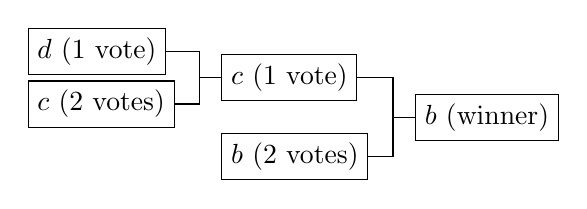
\begin{tikzpicture}%
[ every text node part/.style={draw, align = left, inner sep = 0pt} ]

% Setup for horizontal tree
    % Grow tree to right with nodes placed clockwise(')
    \tikzset{grow'=left}
    % Use edges with 90° bends instead of default straight
    \tikzset{edge from parent/.style = { draw,
             edge from parent path = { (\tikzparentnode.west) 
                                        -- +(-8pt, 0)
                                        |- (\tikzchildnode.east) }}}
    % Increase horizontal spacing (adjust if length of name is long)
    \tikzset{level distance = 7em}
    % Adjust the alignment of the nodes
    \tikzset{every tree node/.style = {draw, anchor = base west}}

\Tree[ .{$b$ (winner)} {$b$ (2 votes)} [ .{$c$ (1 vote)} {$c$ (2 votes)} {$d$ (1 vote)} ] ]
\end{tikzpicture}
\label{f:cc-first-vote}
\caption{One way of running an election for the Condorcet cycle}
\end{figure}

But that's just way of running the election.  What if we switched it around? 

\begin{figure}
\centering
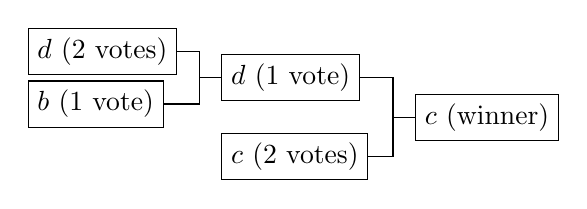
\begin{tikzpicture}%
[ every text node part/.style={draw, align = left, inner sep = 0pt} ]

% Setup for horizontal tree
    % Grow tree to right with nodes placed clockwise(')
    \tikzset{grow'=left}
    % Use edges with 90° bends instead of default straight
    \tikzset{edge from parent/.style = { draw,
             edge from parent path = { (\tikzparentnode.west) 
                                        -- +(-8pt, 0)
                                        |- (\tikzchildnode.east) }}}
    % Increase horizontal spacing (adjust if length of name is long)
    \tikzset{level distance = 7em}
    % Adjust the alignment of the nodes
    \tikzset{every tree node/.style = {draw, anchor = base west}}

\Tree[ .{$c$ (winner)} {$c$ (2 votes)} [ .{$d$ (1 vote)} {$b$ (1 vote)} {$d$ (2 votes)} ] ]
\end{tikzpicture}
\label{f:cc-second-vote}
\caption{A second way of running an election for the Condorcet cycle}
\end{figure}

And, of course, there is a third way

\begin{figure}
\centering
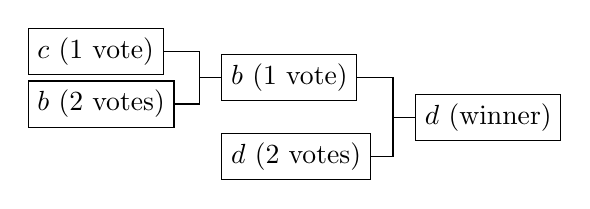
\begin{tikzpicture}%
[ every text node part/.style={draw, align = left, inner sep = 0pt} ]

% Setup for horizontal tree
    % Grow tree to right with nodes placed clockwise(')
    \tikzset{grow'=left}
    % Use edges with 90° bends instead of default straight
    \tikzset{edge from parent/.style = { draw,
             edge from parent path = { (\tikzparentnode.west) 
                                        -- +(-8pt, 0)
                                        |- (\tikzchildnode.east) }}}
    % Increase horizontal spacing (adjust if length of name is long)
    \tikzset{level distance = 7em}
    % Adjust the alignment of the nodes
    \tikzset{every tree node/.style = {draw, anchor = base west}}

\Tree[ .{$d$ (winner)} {$d$ (2 votes)} [ .{$b$ (1 vote)} {$b$ (2 votes)} {$c$ (1 vote)} ] ]
\end{tikzpicture}
\label{f:cc-third-vote}
\caption{A third way of running an election for the Condorcet cycle}
\end{figure}

So now instead of debating which restaurant to go to, each friend will debate the proper way to structure the election. We could have them vote on that, but that's no help because we'll just generate another Condorcet cycle.

The basic problem is this: for any restaurant you choose, the majority will prefer a particular alternative to the one that is chosen.  This happens regardless of which one is chosen, so as a result no particular solution appears ``best.''

\section{What about utilities?}

After we spent all this effort trying to figure out utilities, it might seem natural to use them in this context.  While the Condorcet cycle is perplexing, perhaps we could resolve the problem by asking people not just what is their preference, but by how much they prefer it.  In fact, we do this all the time\dots but maybe we shouldn't?

The first thing to note is that this can't eliminate the Condorcet cycle entirely. We could also specify that everyone's strength of preference is exactly the same and be back where we started.

But, actually there is a deeper problem than this.  Let's suppose that we did the von Neumann\breakslash Morgenstern exercise and discovered that these three utility functions represented Mandy, Evan, and Stephanie's preferences:
\begin{itemize}
    \item Mandy: $u_M(b) = 1$, $u_M(c) = 0.7$, and $u_M(d) = 0$
    \item Evan: $u_E(c) = 2$, $u_E(d) = 1.2$, and $u_E(b) = 0$
    \item Stephanie: $u_S(d) = 10$, $u_S(b) = 0.1$, and $u_S(c) = 0$
\end{itemize}
We {\it could} sum up these numbers and find that the total for $b$ is 1.1, the total for $c$ is 2.7, and the total for $d$ is 11.2. That would suggest that $d$ is the best choice.

Have you noticed the problem?  Recall what we called the ``second representation theorem.''  If each of these functions represent someone's preferences, then we can either add any number or multiply by any positive number and still represent their preferences.  So we could have multiplied Evan's utilities by 100 (say), and then $c$ would have won.  Or any of a number of other things. 

What happens when we add different people's utilities is much like trying to add Celsius and Fahrenheit.  You end up with something strange and meaningless.  So although we can talk about one option having a higher utility for Mandy (or for Evan or for Stephanie), we cannot talk about something having a higher total utility for all three of them.

This problem is called the problem of {\it interpersonal comparison of utility}.

\section{Axiomatizing voting}

The Condorcet cycle represents a problem for making collective choices. One might want to approach this problem from a more systematic way.  In order to do that, we need to think a little bit more about what making a collective choice means.

We've already introduced the idea of a community profile, this is a vector of preference relations: one preference relation for each person in the community.  Now let's consider the set $R^N$, which represents all possible community profiles. This represents all the possible communities (of size $N$) that might exist. Or at least it represents all the ways they might feel about the set $X$.\marginnote{It's important to note that while we will often use examples with strict preferences $\succ$, $R$ includes indifferences too.  The person who doesn't care and is indifferent between all options is in $R$. So too is someone who has some indifferences and some strict preferences.}

Now that we have this on the table, we can think of a mechanism to make a choice, something called a {\it social choice function}.  This is an $f:  R^N \to R$.  A function that takes as input a community profile (what everyone in the community prefers) and returns a single preference relation.

The first thing to note is that there are many functions of this form. There are many ways to make a social decision.  Here are a few extremely bad ones:
\begin{itemize}
    \item $f_1$ is a constant function, regardless of the input it returns the same preference relation
    \item $f_2$ always returns the preference relation of the first person in the community profile
    \item $f_3$ takes the third person's preference relation, reverses it, and returns that
\end{itemize}
Take a moment to think about each of these, and make sure you understand {\it why} almost everyone would think they are a bad idea.

How do we solve this? The basic strategy is to come up with constraints on $f$ that seem intuitively reasonable.  To ruin the ending: several reasonable constraints contradict each other and leave us with nothing.

\section{Arrow's theorem}

The economist Kenneth Arrow is famous for proving his impossibility theorem.  He gives us several axioms or constraints on $f$ that seem intuitively plausible, and then proves that all of them are incompatible.

The first three are ``hidden'' assumptions because they are built into how we define a social choice function.  Both are already assumed when we said that $f$ is a function from $R^N$ to $R$.
\begin{definition}[Social ordering]
The function $f$ outputs a preference relation which is complete and transitive
\end{definition}
This assumption strikes a lot of people as somewhat strong.  Sometimes we don't much care in who is in second, third, and fourth place (although we do sometimes). It is critical that $f$ not output an intransitive ordering.  If we had a cycle then we can't choose a winner.

The second ``hidden'' assumption is more critical. It comes again from the fact that we defined $f$ to be a function from $R^N$ to $R$.
\begin{definition}[Universal domain]
The function $f$ is defined for all members of $R^N$
\end{definition}
This means that our system of social choice is defined {\it no matter what preferences people have}, including the Condorcet cycle (or anything else for that matter).  

The third ``hidden'' assumption is that the voting system does not involve any randomness.  We are assuming that given the same input, $f$ always provides the same output.  It can output indifferences, that we might decide to resolve by flipping a coin.  But it cannot itself flip a coin.  So there is no way for it to, say, choose someone at random to decide the issue (sometimes called ``the random dictator method'').

After these three, the additional assumptions are no longer ``hidden.'' We need to make them explicitly.  For all the conditions that follow we will assume there is an input community profile, $C = \langle \succ_1, \succ_2, \dots, \succ_N\rangle$.  And we'll represent the output as $f(C) = \succ_C$

The first real condition is one that strikes most people as completely reasonable. The social ordering should respect, at the very least, unanimous judgments.  That is, if everyone preference option $x \succ_i y$, then the group must as well.
\begin{definition}[Weak Pareto]
If for any two alternatives $x, y \in X$, if for all $i\in N$ $x \succ_i y$, then $x \succ_C y$
\end{definition}

The next condition is also one that strikes most people as reasonable.  It requires that no one person controls what the social preference is.  
\begin{definition}[Non-dictatorship]
It is not the case that there exists an $i$, such that for all $x$ and $y$, $x \succ_C y$ if and only if $x \succ_i y$
\end{definition}
This is also a pretty weak condition. It only requires that for each person there is at least one pair of outcomes $x$ and $y$ society can overrule that person's preference on that particular pair of outcomes. It does  allow that people can be ``local'' dictators, which we will talk about in a minute.

To talk about the last condition, we need to talk about what it means for two community profiles to {\it agree} on a pair $x, y$.  We will say that two different community profiles $M$ and $M^\prime$ {\it agree} on $x, y$ if no person changes their mind about their preference between $x$ and $y$ between the two profiles.  

Table~\ref{t:sc-agreement} gives an example of two profiles that agree on $x,y$.  Note, however, they they {\bf do not} agree on $x, z$ or $y, z$ since at least one person changes their mind about the relative rankings of those two pairs.
\begin{table}
    \centering
\begin{tabular}{cccc}
    \toprule
     & \multicolumn{3}{c}{People} \\
Profile           & $A$ & $B$ & $C$ \\
           \midrule
$M$        & $x \succ y \succ z$ & $y \succ x \succ z$ & $y \succ z \succ x$ \\
$M^\prime$ & $x \succ z \succ y$ & $z \succ y \succ x$ & $y \succ z \succ x$ \\
\bottomrule
\end{tabular}
\medskip
\caption{Two profiles that agree on $x$ and $y$. They do not agree on $x, z$ or $y, z$, however.}
\label{t:sc-agreement}
\end{table}

With that in hand, we can state the last of the assumptions about $f$. This one is probably the most controversial, and the one we will spend the most time discussing.  So, it's worth making sure you understand it.

\begin{definition}[Independence of Irrelevant Alternatives]
If $M$ and $M^\prime$ are two community profiles that agree on the pair $x, y$, and if $\succsim_C = f(M)$ and $\succsim_C^\prime = f(M^\prime)$, then:
\begin{enumerate} 
\item $x \succsim_C y$ if and only if $x \succsim_C^\prime y$ {\bf and}
\item $y \succsim_C x$ if and only if $y \succsim_C^\prime x$ 
\end{enumerate}
\end{definition}

This is called Independence of Irrelevant Alternatives (IIA for short) because it says that whether $x$ is ranked higher than $y$ or vice versa depends only on how people in the community rank $x$ and $y$ relative to each other.  You can change how they rank any other pair, but if you keep $x$ and $y$ the same for {\it every} individual then you must keep the social ranking the same as well.

With these in hand, we can express Arrow's famous theorem:
\begin{proposition}
There is no $f: R^N \to R$ that obeys Weak Pareto, Non-dictatorship, and Independence of Irrelevant Alternatives.
\end{proposition}
(Of course, the three ``hidden'' assumptions are there as well, they are all contained in the statement of what kind of function $f$ is.)

There are many different ways to prove this theorem.  An economist, John Geanakoplos, has a paper where he presents three of them.\marginnote{For those proofs see \fullcite{Geanakoplos2005}}  In this chapter we will use his second proof, since it makes use of the Condorcet cycles we've already discussed. 

We need to generalize those cycles just a little more since we might have more than three alternatives.  But, I suspect you already see how to do that.  We start by rank ordering the options in $X$, $x_1, x_2, \dots, x_m$.  Now consider a preference ordering $o_i$ that starts with $x_i$ of these and lists the $x$'s in order until it reaches the end and then starts from the top. 
\begin{table}
\centering
    \begin{tabular}{cccc}
    \toprule
    $o_1$ & $o_2$ & \dots & $o_m$ \\
    \midrule
    $x_1$ & $x_2$ & \dots & $x_m$ \\
    $x_2$ & $x_3$ & \dots & $x_1$ \\
    $x_3$ & $x_4$ & \dots & $x_2$ \\
    $\vdots$ & $\vdots$ & $\ddots$ & $\vdots$ \\
    $x_m$ & $x_1$ & \dots & $x_{m-1}$ \\
    \bottomrule
    \end{tabular}
    \medskip
    \caption{The ``Condorcet'' preference relations $o_i$.}
    \label{sc-oi}
\end{table}

A second concept that will be useful is one called {\it a local dictator}. A person is a local dictator at $M$ if {\it for any pair} of outcomes $x$ and $y$ they can make the community adopt $x \succ y$ by changing their preference to some other preference where $x \succ y$ {\it while everyone else stays the same}.  The idea is that at $M$, this person is a dictator.  That doesn't necessarily mean they are a dictator everywhere, just locally at $M$.

With this in hand, we can start the proof.  The proof will work as follows, it will show that any $f$ which obeys Weak Pareto and IIA must have a dictator (thus proving the three are incompatible).

To do this we will break the proof into several steps.
\begin{itemize}
    \item Step 1: We will start with one particular preference profile, which we call $M$.  We will show that at $M$ there is a local dictator.
    \item Step 2: We will show that if someone is a local dictator at a profile, then they are a local dictator at a nearby profile constructed by only one person changing one outcome by a ``half step.''
    \item Step 3: We will observe that you can go from $M$ to any profile by a series of ``half steps.'' Establishing that the local dictator at $M$ must also be a global dictator
\end{itemize}

% There is a little diagram I have in mind for the constructions I do in this proof

%
%  MD ----> ME
%   |        |
%   v        v
%  MD1       ME1

% I don't have time to do this now, but I think it would help in the future.

% Maybe also a similar thing for Mi and M-.  These are a little trickier.

% There's also the lacuna in the proof (what if there is no \gamma that is unrelated to the \alpha,\beta, maybe I should think about how to deal with that.

% I also think that the Step 1 of the proof isn't quite clear about what it's proving at each step.  I think it's worth being a little more careful

\begin{proof}
~\\
\noindent \textbf{Step 1}

Suppose that every $\succsim_i$ equals $o_1$. By Weak Pareto, we know that community profile in such a case must also equal $o_1$. Therefore there is at least one profile that involves only the Condorcet preference relations and results in $o_1$ the social ordering.  

Now let $M$ be the community profile that involves only the Condorcet Profiles and has the minimum number of people with preference $o_1$ such that the resulting community preference relation is $\succsim^M = o_1$. There must be at least one person who has $o_1$, since otherwise Weak Pareto would require that $o_m \succ o_1$.  Let $n^*$ be a person in $M$ with profile $o_1$.

What we will now show is that person $n^*$ is a local dictator at $M$.  To do this, we have to show that $n^*$ can change the social rank of any pair by changing her own ranking. 

Suppose that $n^*$ changes there preference from $o_1$ to $o_i$ for some $i$. Call this new profile $M^i$ and the resulting preference relation $\succsim^i$ Because we required that preference relation $M$ had the minimum number of people for the result to be $\succsim^M = o_1$, then we know that $\succsim^i \ne o_1$ under this new profile.  We know that $M^i$ and $M$ agree on all pairs $x_1, x_2, \dots, x_{i-1}$. So, by IIA $\succsim^i$ must rank those objects the same as in $o_1$.  Similarly, $M^i$ and $M$ agree on all pairs $x_i, x_{i+1}, \dots, x_m$.  So again by IIA, those must stay the same as in $o_1$.  Something has to change, and so that must be $x_i \succsim^i x_{i-1}$.  
What we have shown so far is that for any $i$, if $n^*$ changes to profile $o_i$, then the resulting social ordering $\succsim^i$ will switch from $x_{i-1} \succ^M x_{i}$ to $x_{i} \succsim^i x_{i-1}$. Notice that our choice of $i$ was arbitrary, so we know that $n^*$ can (weakly) reverse the preference between any neighboring pair of $x_{i-1}, x_i$.

Now consider a different change for $n^*$.  Let $o_1^-$ be the profile where $n^*$ adopts the exact opposite of $o_1$, namely that $x_m \succ x_{m-1} \succ \dots \succ x_2 \succ x_1$. Let $M^-$ be the social profile where everyone else adopts the same preferences as in $M$, but where $n^*$ adopts $o_1^-$ and let $\succsim^-$ be the resulting social preference relation. Consider each consecutive pair of outcomes $x_{i-1}, x_i$.  $M^-$ agrees with $M^i$ about that pair. By the previous argument, we know that $\succ^i$ ranks them  $x_i \succsim^i x_{i-1}$, so $M^-$ must also rank them  $x_i \succsim^- x_{i-1}$.  Since that's true for all consecutive pairs, we know that $x_m \succsim^- x_{m-1} \succsim^- \dots \succsim^- x_2 \succsim^- x_1$.

So far what we've shown is that $n^*$ can move a strict preference in one direction to a weak one in the other direction. To establish that $n^*$ is a local dictator, we have to show that this is a strict social preference.  Suppose that for some pair $x_i \sim^- x_{i-1}$. By IIA, this will imply that $x_i \sim^i x_{i-1}$ (since $M^-$ and $M^i$ agree on that pair).  Recall that $M^i$ and $M$ agree on all pairs of objects $x_1, x_2, \dots x_{i-1}$ and also on all pairs of objects $x_i, x_{i+1}, \dots, x_m$.  So that must mean that $\succ^i$ ranks them $x_1 \succ^i x_2 \succ^i \dots \succ^i x_{i-1}$  and $x_i \succ^i x_{i+1} \succ^i \dots \succ^i x_m$.  If $x_i \sim^i x_{i-1}$, then by transitivity, $x_1 \succ^i x_m$. Since $M^i$ and $M^-$ agree on the pair $x_1, x_m$, then by IIA this implies that $x_1 \succ^- x_m$ which contradicts that $x_m \succsim x_1$. 

So, it cannot be the case that for any $i$, $x_i \sim^- x_{i-1}$.  Therefore $x_m \succ^i x_{m-1} \succ^i \dots \succ^i x_2 \succ^i x_1$. This establishes that $n^*$ is a local dictator at $M$ since they can reverse the social preference between any pair.

~\\
\noindent \textbf{Step 2}

Now, we have to show that the fact that $n^*$ is a local dictator at $M$ shows that they are a global dictator (that their profile is always chosen by $f$).  

Let $M^D$ be a profile where $n^*$ is a local dictator. (We know this exists because $M$ is such a profile.) Let $\succsim^D$ be the resulting social order at $M^D$. Consider a new profile $M^E$ where one $n \ne n^*$ changes one element of $X$ by one ``half-step.''  (That is, $n$ either breaks an indifference or introduces a new one, but not both.)  Let $\succsim^E$ be the social preference order at $M^E$.

We will now show that $n^*$ is a local dictator at $M^E$ also.  Let $\alpha$ and $\beta$ be two elements in $X$ that are changed in moving from $M^D$ to $M^E$. 

First, suppose that $\gamma \succ^E \delta$ for two elements neither of which are $\alpha$ or $\beta$.  By IIA we know that $\gamma \succ^D \delta$ as well. Because $n^*$ is a local dictator, we know that at $M^D$ there is some profile that can be adopted by $n^*$ such that $\delta \succ_{n^*} \gamma$ and this can force the social order to respect that.  Call this new profile $M^{D1}$ where $\delta \succ^{D1} \gamma$.  Now consider the same change by $n^*$ in $M^E$ and call that $M^{E1}$.  Notice that $M^{D1}$ and $M^{E1}$ agree on the pair $\delta, \gamma$.  So, by IIA, $\gamma \succ^{E1} \delta$. This establishes that $n^*$ can force their preference for $\delta$ and $\gamma$ onto the social order.

The only remaining three pairs to consider are those involving $\alpha$ and $\beta$.  Let $\gamma$ be an element where there is no change in its relationship to $\alpha$ and $\beta$. (It is possible that there is no $\gamma$, but this is a very special circumstance. I'll leave that case for you to think about on your own.)

Since $n^*$ is a local dictator, there is some change they can make such that $\alpha \succ_{n^*} \gamma$ and this is forced on the community.  Call this profile $M^{D2}$ where $\alpha \succ^{D2} \gamma$. 

Now make a second change by $n^*$ to make $\gamma \succ_{n*} \beta$.  Call this $M^{D3}$.  Because $n^*$ is a dictator at $M^D$ and IIA, then we know that $M^{D3}$ matches that $\gamma \succ^{D3} \beta$

Now we'll do the same thing again, but starting at $M^{E}$. Similarly let $M^{E3}$ be the profile where $n^*$ makes those same changes, $\alpha \succ_{n^*} \gamma \succ_{^n*} \beta$.  Since $M^{D3}$ and $M^{E3}$ agree on the pairs $\alpha, \gamma$ and $\beta, \gamma$, then it must also be the case that $\alpha \succ^{E3} \gamma \succ^{E3} \beta$ and by transitivity $\alpha \succ^{E3} \beta$. This shows that $n^*$ is a local dictator at $M^E$ also.

~\\
\noindent \textbf{Step 3}

The last step in the proof is to observe that we can get to any community profile through a series of half steps of this form.  So, for any profile, we can establish that $n^*$ is a local dictator.  Therefore, $n^*$ is a global dictator.

\end{proof}

Phew.  That's a long and somewhat complicated proof.  It turns out that there isn't a really easy way to show it, and this is---in my opinion---one of the clearer ones.  To be honest, I even find it hard to make intuitive. So if you are struggling with that, you aren't alone.

What should we make of this?  Well, this shows that our plausible constraints can't be jointly satisfied. So we have to give up on at least one of them.

Weak pareto and non-dictator are usually regarded as so reasonable as to be above reproach.  More common one's to consider are IIA, Universal Domain, and non-randomness.

Non-randomness would allow for a choice system that chose either a voter or the options at random.  The ``random dictator'' rule choose from among the voters who gets to be a dictator today, and then chooses whatever they prefer.  Or, the ``random options'' rule chooses two options at random and then picks the one that the majority wants. There are actually some strange reasons why these rules might be good ideas, but we won't have time to go into them here.

Violating universal domain is sometimes discussed.  It turns out that if you exclude certain possible combinations of preference relations, then you can satisfy all the other conditions.  One famous one is called a ``single peaked'' preference relation where the options are arranged on a line and people form preferences by choosing a point on the line and organizing their preferences by looking at how far an option is away from their ideal point.  If we are assured the voters preferences are arranged in this way, then majority vote obeys all of Arrow's other conditions.

Finally, we come to IIA. Some common ways of voting violate this constraint. Let's look at one common way of voting to see why.  The ``Borda count'' is a way of voting that you probably have used before, but you might not know it's name.  Under the Borda count people vote with their full preference ranking.  Each first place vote is worth one point, each second is worth two points, etc.  The candidate who has the {\it lowest} number of points (like golf) wins.

\begin{table}
\centering
    \begin{tabular}{cccccc}
    \toprule
      & \multicolumn{5}{c}{\bf Options} \\ \cmidrule(lr){2-6}
       {\bf Voter} & $o_1$ & $o_2$ & $o_3$ & $o_4$ & $o_5$ \\
            \midrule
    $V_1$   & 1 & 2 & 3 & 4 & 5 \\
    $V_2$   & 2 & 3 & 4 & 5 & 1 \\
    $V_3$   & 1 & 2 & 4 & 3 & 5 \\
    $V_4$   & 2 & 5 & 4 & 3 & 1 \\
    $V_5$   & 2 & 3 & 5 & 4 & 1 \\
    \midrule
    {\bf Total} & 8 & 15 & 20 & 19 & 13 \\     
     \bottomrule
    \end{tabular}
    \medskip
    \label{t:borda-IIA}
    \caption{An illustration of the Borda count.}
\end{table}
Under the Borda count this community would rank the options $o_1 \succ o_5 \succ o_2 \succ o_4 \succ o_3$.  Now let's consider another community with voters $V^\prime_1 - V^\prime_5$.  Notice that the $V^\prime$-voters agree with the $V$-voters on their ranking of $o_1$ and $o_5$.  (Remember what that means! Voters $V_1$, $V_3$, $V_1^\prime$, $V_3^\prime$ all rank $o_1 \succ o_5$ and the rest rank $o_5 \succ o_2$)

\begin{table}
\centering
    \begin{tabular}{cccccc}
    \toprule
      & \multicolumn{5}{c}{\bf Options} \\ \cmidrule(lr){2-6}
       {\bf Voter} & $o_1$ & $o_2$ & $o_3$ & $o_4$ & $o_5$ \\
            \midrule
    $V_1^\prime$   & 1 & 5 & 3 & 4 & 2 \\
    $V_2^\prime$   & 5 & 3 & 4 & 2 & 1 \\
    $V_3^\prime$   & 1 & 5 & 4 & 3 & 2 \\
    $V_4^\prime$   & 5 & 2 & 4 & 3 & 1 \\
    $V_5^\prime$   & 5 & 3 & 2 & 4 & 1 \\
    \midrule
    {\bf Total} & 17 & 18 & 16 & 16 & 7 \\     
     \bottomrule
    \end{tabular}
    \medskip
    \label{t:borda-IIA-prime}
    \caption{An illustration of the Borda count violating IIA.}
\end{table}

Now the Borda count generates a ranking $o_5 \succ o_3 \sim o_4 \succ o_1 \succ o_2$.  Of critical importance here is that now $o_5 \succ o_2$ despite the fact that no one changed their relative ranking of these two options.  

People who like Borda count (or other voting schemes) have to argue that IIA is an unreasonable constraint. But, of course, there is a some shred of reasonableness to it.  So people have sought variations that {\it can} be satisfied.  There are many different ways to replace IIA with similar, but somewhat weaker, conditions.  Unfortunately, there are a lot of them and they disagree with each other. So the state of the art is now debating which way of weakening IIA is the most reasonable.

\section{Conclusion}

As you might imagine, there is so much more we could say.  Whole books have been written about social choice.  If this strikes you as an interesting topic, there is much you can learn.

The basic point is that democracy is harder than it looks.  What is ``the will of the people'' is not well defined.  We must make choices about how to aggregate preferences, and however we do it, it will be controversial.  Attempts to make one-sized-fits-all decision rules for democracy are bound to be hard.  The difficulty is worth it, of course, but we should understand that it is\dots indeed\dots difficult.

% No list of symbols at the end
%\printnomenclature

\backmatter

\printbibliography

\end{document}
